\documentclass[a4paper,onecolumn,oneside,12pt,extrafontsizes]{memoir}
\usepackage[cp1250]{inputenc}
\usepackage[T1]{fontenc}
\usepackage[polish]{babel}
%\DisemulatePackage{setspace}
\usepackage{setspace}
\usepackage{tabularx}
\usepackage[cache=false, newfloat]{minted}
\usepackage{caption}
\usepackage{longtable}
\usepackage{color,calc}
%\usepackage{soul} % pakiet z komendami do podkreślania tekstu
\usepackage{ebgaramond}
\usepackage{tgtermes}   
\renewcommand*\ttdefault{txtt}
\usepackage{listings} 
\newcommand{\listingcaption}[1]
{%
\vspace*{\abovecaptionskip}\small 
\refstepcounter{lstlisting}\hfill%
Listing \thelstlisting: #1\hfill%\hfill%
\addcontentsline{lol}{lstlisting}{\protect\numberline{\thelstlisting}#1}
}%

% Styl zapewniający numerowanie linii
\lstset{
  basicstyle=\footnotesize\ttfamily,
  columns=fullflexible,
	showstringspaces=false,
	showspaces=false,
  breaklines=true,
  postbreak=\mbox{\textcolor{red}{$\hookrightarrow$}\space},
  numbers=left,
  firstnumber=1,
  numberfirstline=true,
	xleftmargin=17pt,
  framexleftmargin=17pt,
  framexrightmargin=5pt,
  framexbottommargin=4pt,
	belowskip=.5\baselineskip
}

% Styl bez numerownia linii
%%\lstset{
  %%basicstyle=\footnotesize\ttfamily,
  %%columns=fullflexible,
	%%showstringspaces=false,
	%%showspaces=false,
  %%breaklines=true,
  %%postbreak=\mbox{\textcolor{red}{$\hookrightarrow$}\space},
%%}

%% Poniżej sposób ostylowania sposobu podświetlania składni wybranych języków
\lstloadlanguages{C,C++,csh,Java}
\definecolor{listingBg}{RGB}{233,232,233}

\lstdefinelanguage{JavaScript}{
  morekeywords={typeof, async, await, new, true, false, catch, function, return, null, catch, switch, var, if, in, while, do, else, case, break},
	otherkeywords={typeof, async, await, new, true, false, catch, function, return, null, catch, switch, var, if, in, while, do, else, case, break},
	tabsize=2, 
  morecomment=[s]{/*}{*/},
  morecomment=[l]//,
  morestring=[b]",
  morestring=[b]',
	numbers=left, 
	numberstyle=\tiny, 
	numbersep=5pt, 
	backgroundcolor=\color{listingBg}
}

\lstdefinestyle{sharpcstyle}{
language=csh,
basicstyle=\footnotesize\ttfamily, 
numbers=left, 
numberstyle=\tiny, 
numbersep=5pt, 
tabsize=2, 
extendedchars=true, 
breaklines=true, 
showspaces=false, 
showtabs=false, 
xleftmargin=17pt,
framexleftmargin=17pt,
framexrightmargin=5pt,
framexbottommargin=4pt,
morecomment=[l]{//}, %use comment-line-style!
morecomment=[s]{/*}{*/}, %for multiline comments
showstringspaces=false,
otherkeywords={ abstract, async, await, var, event, new, struct,
explicit, null, switch,
base, extern, object, this,
bool, false, operator, throw,
break, finally, out, true,
byte, fixed, override, try,
case, float, params, typeof,
catch, for, private, uint,
char, foreach, protected, ulong,
checked, goto, public, unchecked,
class, if, readonly, unsafe,
const, implicit, ref, ushort,
continue, in, return, using,
decimal, int, sbyte, virtual,
default, interface, sealed, volatile,
delegate, internal, short, void,
is, sizeof, while,
double, lock, stackalloc,
else, long, static,
enum, namespace, string},
morekeywords={ abstract, async, await, var, event, new, struct, 
explicit, null, switch,
base, extern, object, this,
bool, false, operator, throw,
break, finally, out, true,
byte, fixed, override, try,
case, float, params, typeof,
catch, for, private, uint,
char, foreach, protected, ulong,
checked, goto, public, unchecked,
class, if, readonly, unsafe,
const, implicit, ref, ushort,
continue, in, return, using,
decimal, int, sbyte, virtual,
default, interface, sealed, volatile,
delegate, internal, short, void, 
is, sizeof, while,
double, lock, stackalloc,
else, long, static,
enum, namespace, string},
backgroundcolor=\color{listingBg}
}

\renewcommand\lstlistlistingname{Spis listingów}
\makeatletter
\g@addto@macro\insertchapterspace{\addtocontents{lol}{\protect\addvspace{10pt}}}
\renewcommand*{\l@lstlisting}{\@dottedtocline{1}{0em}{2.3em}}
\makeatother
\renewcommand*{\lstlistlistingname}{Spis listingów} \newlistof{lstlistoflistings}{lol}{\lstlistlistingname}

%\hyphenpenalty=10000		% nie dziel wyrazów zbyt często
\clubpenalty=10000      %kara za sierotki
\widowpenalty=10000  % nie pozostawiaj wdów
%\brokenpenalty=10000		% nie dziel wyrazów między stronami - trzeba było wyłączyć, bo nie łamały się linie w lstlisting
%\exhyphenpenalty=999999		% nie dziel słów z myślnikiem - trzeba było wyłączyć, bo nie łamały się linie w lstlisting
\righthyphenmin=3			% dziel minimum 3 litery
%\tolerance=4500
%\pretolerance=250
%\hfuzz=1.5pt
%\hbadness=1450

\renewcommand{\topfraction}{0.95}
\renewcommand{\bottomfraction}{0.95}
\renewcommand{\textfraction}{0.05}
\renewcommand{\floatpagefraction}{0.35}

%%%%%%%%%%%%%%%%%%%%%%%%%%%%%%%%%%%%%%%%%%%%%%%%%%%
%%  Ustawienia rozmiarów: tekstu, nagłówka i stopki, marginesów
%%  dla dokumentów klasy memoir 
%%%%%%%%%%%%%%%%%%%%%%%%%%%%%%%%%%%%%%%%%%%%%%%%%%%
\setlength{\headsep}{10pt} 
\setlength{\headheight}{13.6pt} % wartość baselineskip dla czcionki 11pt tj. \small wynosi 13.6pt
\setlength{\footskip}{\headsep+\headheight}
\setlength{\uppermargin}{\headheight+\headsep+1cm}
\setlength{\textheight}{\paperheight-\uppermargin-\footskip-1.5cm}
\setlength{\textwidth}{\paperwidth-5cm}
\setlength{\spinemargin}{2.5cm}
\setlength{\foremargin}{2.5cm}
\setlength{\marginparsep}{2mm}
\setlength{\marginparwidth}{2.3mm}
%\settrimmedsize{297mm}{210mm}{*}
%\settrims{0mm}{0mm}	
\checkandfixthelayout[fixed] % konieczne, aby się dobrze wszystko poustawiało
%%%%%%%%%%%%%%%%%%%%%%%%%%%%%%%%%%%%%%%%%%%%%%%%
%%  Ustawienia odległości linii, wcięć, odstępów
%%%%%%%%%%%%%%%%%%%%%%%%%%%%%%%%%%%%%%%%%%%%%%%%
\linespread{1}
%\linespread{1.241}
\setlength{\parindent}{14.5pt}
%\setlength{\cftbeforechapterskip}{0.3em} % odstępy w spisie treści
%\setbeforesecskip{10pt plus 0.5ex}%{-3.5ex \@plus -1ex \@minus -.2ex}
%\setaftersecskip{10pt plus 0.5ex}%\onelineskip}
%\setbeforesubsecskip{8pt plus 0.5ex}%{-3.5ex \@plus -1ex \@minus -.2ex}
%\setaftersubsecskip{8pt plus 0.5ex}%\onelineskip}
%\setlength\floatsep{6pt plus 2pt minus 2pt} 
%\setlength\intextsep{12pt plus 2pt minus 2pt} 
%\setlength\textfloatsep{12pt plus 2pt minus 2pt} 
\usepackage{memlays}     % extra layout diagrams, zastosowane w szblonie do 'debuggowania', używa pakietu layouts
%\usepackage{layouts}
\usepackage{printlen} % pakiet do wyświetlania wartości zdefiniowanych długości, stosowany do 'debuggowania'
\uselengthunit{pt}
\makeatletter
\newcommand{\showFontSize}{\f@size pt} % makro wypisujące wielkość bieżącej czcionki
\makeatother
% do pokazania ramek można byłoby użyć:
%\usepackage{showframe} 
%%%%%%%%%%%%%%%%%%%%%%%%%%%%%%%%%%%%%%%%%%%%%%%%%%%
%%  Formatowanie list wyliczeniowych, wypunktowań i własnych otoczeń
%%%%%%%%%%%%%%%%%%%%%%%%%%%%%%%%%%%%%%%%%%%%%%%%%%%

% Domyślnie wypunktowania mają zadeklatorowane znaki, które nie występują w tgtermes
% Aby latex nie podstawiał w ich miejsca znaków z czcionki standardowej można zrobić podstawienie:
%    \DeclareTextCommandDefault{\textbullet}{\ensuremath{\bullet}}
%    \DeclareTextCommandDefault{\textasteriskcentered}{\ensuremath{\ast}}
%    \DeclareTextCommandDefault{\textperiodcentered}{\ensuremath{\cdot}}
% Jednak jeszcze lepszym pomysłem jest zdefiniowanie otoczeń z wykorzystaniem enumitem
\usepackage{enumitem} % pakiet pozwalający zarządzać formatowaniem list wyliczeniowych
\setlist{noitemsep,topsep=4pt,parsep=0pt,partopsep=4pt,leftmargin=*} % zadeklarowane parametry pozwalają uzyskać 'zwartą' postać wypunktowania bądź wyliczenia
\setenumerate{labelindent=0pt,itemindent=0pt,leftmargin=!,label=\arabic*.} % można zmienić \arabic na \alph, jeśli wyliczenia mają być z literkami
\setlistdepth{4} % definiujemy głębokość zagnieżdżenia list wyliczeniowych do 4 poziomów
\setlist[itemize,1]{label=$\bullet$}  % definiujemy, jaki symbol ma być użyty w wyliczeniu na danym poziomie
\setlist[itemize,2]{label=\normalfont\bfseries\textendash}
\setlist[itemize,3]{label=$\ast$}
\setlist[itemize,4]{label=$\cdot$}
\renewlist{itemize}{itemize}{4}

%%%http://tex.stackexchange.com/questions/29322/how-to-make-enumerate-items-align-at-left-margin
%\renewenvironment{enumerate}
%{
%\begin{list}{\arabic{enumi}.}
%{
%\usecounter{enumi}
%%\setlength{\itemindent}{0pt}
%%\setlength{\leftmargin}{1.8em}%{2zw} % 
%%\setlength{\rightmargin}{0zw} %
%%\setlength{\labelsep}{1zw} %
%%\setlength{\labelwidth}{3zw} % 
%\setlength{\topsep}{6pt}%
%\setlength{\partopsep}{0pt}%
%\setlength{\parskip}{0pt}%
%\setlength{\parsep}{0em} % 
%\setlength{\itemsep}{0em} % 
%%\setlength{\listparindent}{1zw} % 
%}
%}{
%\end{list}
%}

\makeatletter
\renewenvironment{quote}{
	\begin{list}{}
	{
	\setlength{\leftmargin}{1em}
	\setlength{\topsep}{0pt}%
	\setlength{\partopsep}{0pt}%
	\setlength{\parskip}{0pt}%
	\setlength{\parsep}{0pt}%
	\setlength{\itemsep}{0pt}
	}
	}{
	\end{list}}
\makeatother

%%%%%%%%%%%%%%%%%%%%%%%%%%%%%%%%%%%%%%%%%
%%  Pakiet do generowania indeksu (ważne, aby wstawić przed hyperref)
%%%%%%%%%%%%%%%%%%%%%%%%%%%%%%%%%%%%%%%%%
\DisemulatePackage{imakeidx}
\usepackage[makeindex,noautomatic]{imakeidx} % tutaj mówimy, żeby indeks nie generował się automatycznie, 

%\usepackage[noautomatic]{imakeidx} 
\makeindex

\makeatletter
%%%\renewenvironment{theindex}
							 %%%{\vskip 10pt\@makeschapterhead{\indexname}\vskip -3pt%
								%%%\@mkboth{\MakeUppercase\indexname}%
												%%%{\MakeUppercase\indexname}%
								%%%\vspace{-3.2mm}\parindent\z@%
								%%%\renewcommand\subitem{\par\hangindent 16\p@ \hspace*{0\p@}}%%
								%%%\phantomsection%
								%%%\begin{multicols}{2}
								%%%%\thispagestyle{plain}
								%%%\parindent\z@                
								%%%%\parskip\z@ \@plus .3\p@\relax
								%%%\let\item\@idxitem}
							 %%%{\end{multicols}\clearpage}
%%%
\makeatother


\usepackage{ifpdf}
%\newif\ifpdf \ifx\pdfoutput\undefined
%\pdffalse % we are not running PDFLaTeX
%\else
%\pdfoutput=1 % we are running PDFLaTeX
%\pdftrue \fi
\ifpdf
 \usepackage[pdftex,bookmarks,breaklinks,unicode]{hyperref}
 \usepackage[pdftex]{graphicx}
 \DeclareGraphicsExtensions{.pdf,.jpg,.mps,.png}
\pdfcompresslevel=9
\pdfoutput=1
\makeatletter
\AtBeginDocument{  % Poniżej zdefiniowano metadane, jakie zapisane zostaną w dokumencie pdf - należy je właściwie uzupełnić
  \hypersetup{
	pdfinfo={
    Title = {\@title},
    Author = {\@author},
    Subject={\@title},
    Keywords={analiza wydajnościowa, interfejsy programowania aplikacji, testowanie rozproszone, wirtualizacja środowisk uruchamiania oprogramowania, środowisko .net, silnik nodejs},  
		Producer={Maciej Grzela},
		Creator={Maciej Grzela}
	}}
}
\pdftrailerid{}
\pdfsuppressptexinfo15
\makeatother
\else
\usepackage{graphicx}
\DeclareGraphicsExtensions{.eps,.ps,.jpg,.mps,.png}
\fi
\sloppy

%\graphicspath{{rys01/}{rys02/}}


%%%%%%%%%%%%%%%%%%%%%%%%%%%%%%%%%%%%%%%%%
% Metadane dla pdfa


%\ifpdf
%\pdfinfo{
   %/Author (Nicola Talbot)
   %/Title  (Creating a PDF document using PDFLaTeX)
   %/CreationDate (D:20040502195600)
   %/ModDate (D:\pdfdate)
   %/Subject (PDFLaTeX)
   %/Keywords (PDF;LaTeX)
%}
%\fi

\usepackage{rotating}

% Deklaracja głębokościu numeracji
\setcounter{secnumdepth}{2}
\setcounter{tocdepth}{2}
\setsecnumdepth{subsection} % activating subsubsec numbering in doc


% Kropki po numerach sekcji
\makeatletter
\def\@seccntformat#1{\csname the#1\endcsname.\quad}
\def\numberline#1{\hb@xt@\@tempdima{#1\if&#1&\else.\fi\hfil}}
\makeatother

\renewcommand{\chapternumberline}[1]{#1.\quad}
\renewcommand{\cftchapterdotsep}{\cftdotsep}


% Czcionka do podpisów tabel i rysunków
\captionnamefont{\small}
\captiontitlefont{\small}
% makro pozwalające zmienić sposób wypisywania rozdziału
%\def\printchaptertitle##1{\fonttitle \space \thechapter.\space ##1} 

%\usepackage{ltcaption}
% The ltcaption package supports \CaptionLabelFont & \CaptionTextFont introduced by the NTG document classes
%\renewcommand\CaptionLabelFont{\small}
%\renewcommand\CaptionTextFont{\small}

% Przedefiniowanie etykiet w podpisach tabel i rysunków
%\AtBeginDocument{% 
        \addto\captionspolish{% 
        \renewcommand{\tablename}{Tab.}% 
}%} 

%\AtBeginDocument{% 
%        \addto\captionspolish{% 
%        \renewcommand{\chaptername}{Rozdział}% 
%}} 

%\AtBeginDocument{% 
        \addto\captionspolish{% 
        \renewcommand{\figurename}{Rys.}% 
}%}


%\AtBeginDocument{% 
        \addto\captionspolish{% 
        \renewcommand{\bibname}{Literatura}% 
}%}

%\AtBeginDocument{% 
        \addto\captionspolish{% 
        \renewcommand{\listfigurename}{Spis rysunków}% 
}%}

%\AtBeginDocument{% 
        \addto\captionspolish{% 
        \renewcommand{\listtablename}{Spis tabel}% 
}%}

%\AtBeginDocument{% 
        \addto\captionspolish

%%%%%%%%%%%%%%%%%%%%%%%%%%%%%%%%%%%%%%%%%%%%%%%%%%%%%%%%%%%%%%%%%%                  
%% Definicje stopek i nagłówków
%%%%%%%%%%%%%%%%%%%%%%%%%%%%%%%%%%%%%%%%%%%%%%%%%%%%%%%%%%%%%%%%%%                  
\addtopsmarks{headings}{%
\nouppercaseheads % added at the beginning
}{%
\createmark{chapter}{both}{shownumber}{}{. \space}
%\createmark{chapter}{left}{shownumber}{}{. \space}
\createmark{section}{right}{shownumber}{}{. \space}
}%use the new settings

\makeatletter
\copypagestyle{outer}{headings}
\makeoddhead{outer}{}{}{\small\itshape\rightmark}
\makeevenhead{outer}{\small\itshape\leftmark}{}{}
\makeoddfoot{outer}{\small\@author:~\@titleShort}{}{\small\thepage}
\makeevenfoot{outer}{\small\thepage}{}{\small\@author:~\@title}
\makeheadrule{outer}{\linewidth}{\normalrulethickness}
\makefootrule{outer}{\linewidth}{\normalrulethickness}{2pt}
\makeatother

% fix plain
\copypagestyle{plain}{headings} % overwrite plain with outer
\makeoddhead{plain}{}{}{} % remove right header
\makeevenhead{plain}{}{}{} % remove left header
\makeevenfoot{plain}{}{}{}
\makeoddfoot{plain}{}{}{}

\copypagestyle{empty}{headings} % overwrite plain with outer
\makeoddhead{empty}{}{}{} % remove right header
\makeevenhead{empty}{}{}{} % remove left header
\makeevenfoot{empty}{}{}{}
\makeoddfoot{empty}{}{}{}


%%%%%%%%%%%%%%%%%%%%%%%%%%%%%%%%%%%%%%%
%% Definicja strony tytułowej 
%%%%%%%%%%%%%%%%%%%%%%%%%%%%%%%%%%%%%%%
\makeatletter
%Uczelnia
\newcommand\uczelnia[1]{\renewcommand\@uczelnia{#1}}
\newcommand\@uczelnia{Politechnika Wrocławska}
%Wydział
\newcommand\wydzial[1]{\renewcommand\@wydzial{#1}}
\newcommand\@wydzial{Wydział Informatyki i Telekomunikacji}
%Kierunek
\newcommand\kierunek[1]{\renewcommand\@kierunek{#1}}
\newcommand\@kierunek{Informatyka}
%Specjalność
\newcommand\specjalnosc[1]{\renewcommand\@specjalnosc{#1}}
\newcommand\@specjalnosc{Systemy i Sieci Komputerowe}
%Tytuł po angielsku
\newcommand\titleEN[1]{\renewcommand\@titleEN{#1}}
\newcommand\@titleEN{Performance analysis of C\# and NodeJS APIs}
%Tytuł krótki
\newcommand\titleShort[1]{\renewcommand\@titleShort{#1}}
\newcommand\@titleShort{Analiza wydajnościowa interfejsów API w technologiach C\# oraz NodeJS}
%Promotor
\newcommand\promotor[1]{\renewcommand\@promotor{#1}}
\newcommand\@promotor{dr inż. Michał Kucharzak}
%Katedra
\newcommand\katedra[1]{\renewcommand\@katedra{#1}}
\newcommand\@katedra{Katedra Systemów i Sieci Komputerowych}

%\usepackage[absolute]{textpos} % zamarkowano, bo ostatecznie wykorzystano otoczenie picture

\def\maketitle{%
  \pagestyle{empty}%
%%\garamond 
	\fontfamily{\ebgaramond@family}\selectfont % na stronie tytułowej czcionka garamond
%%%%%%%%%%%%%%%%%%%%%%%%%%%%%%%%%%%%%	
%% Poniżej, w otoczniu picture, wstawiono tytuł i autora. 
%% Tytuł (z autorem) musi znaleźć się w obszarze 
%% odpowiadającym okienku 110mmx75mm, którego lewy górny róg 
%% jest w położeniu 77mm od lewej i 111mm od górnej  krawędzi strony 
%% (tak wynika z wycięcia na okładce). 
%% Poniższy kod musi być użyty dokładnie w miejscu gdzie jest.
%% Jeśli tytuł nie mieści się w okienku, to należy tak pozmieniać 
%% parametry użytych komend, aby ten przydługi tytuł jednak 
%% upakować go do okienka.
%%
%% Sama okładka (kolorowa strona z wycięciem, do pobrania z dydaktyki) 
%% powinna być przycięta o 3mm od każdej z krawędzi.
%% Te 3mm pewnie zostawiono na ewentualne spady czy też specjalną oprawę.
%%%%%%%%%%%%%%%%%%%%%%%%%%%%%%%%%%%%%	
\newlength{\tmpfboxrule}
\setlength{\tmpfboxrule}{\fboxrule}
\setlength{\fboxsep}{2mm}
\setlength{\fboxrule}{0mm} 
%\setlength{\fboxrule}{0.1mm} %% jeśli chcemy zobaczyć ramkę
\setlength{\unitlength}{1mm}
\begin{picture}(0,0)
\put(26,-124){\fbox{
\parbox[c][71mm][c]{104mm}{\centering%\lineskip=34pt 
\fontsize{18pt}{18pt}\selectfont \@title\\[5mm]
\fontsize{18pt}{18pt}\selectfont \@titleEN\\[20mm]
\fontsize{16pt}{18pt}\selectfont AUTOR:\\[2mm]
\fontsize{15pt}{16pt}\selectfont \@author}
}
}
\end{picture}
\setlength{\fboxrule}{\tmpfboxrule} 
%%%%%%%%%%%%%%%%%%%%%%%%%%%%%%%%%%%%%
%% Reszta strony z nazwą uczelni, wydziału, kierunkiem, specjalnością
%% promotorem, oceną pracy, miastem i rokiem
	{\centering%\vspace{-1cm}
		{\fontsize{22pt}{24pt}\selectfont \@uczelnia}\\[0.4cm]
		{\fontsize{18pt}{20pt}\selectfont \@wydzial}\\[0.5cm]
		  \hrule %\vspace*{0.7cm}
	}
{\flushleft\fontsize{14pt}{16pt}\selectfont%
\begin{tabular}{ll}
KIERUNEK: & \@kierunek\\
SPECJALNOŚĆ: & \@specjalnosc\\
\end{tabular}\\[1.3cm]
}
{\centering
{\fontsize{32pt}{36pt}\selectfont PRACA DYPLOMOWA}\\[0.5cm]
{\fontsize{32pt}{36pt}\selectfont MAGISTERSKA}\\[2.5cm]
}
\vfill
\begin{tabularx}{\linewidth}{p{6cm}X}
		&{\fontsize{16pt}{18pt}\selectfont PROWADZĄCY PRACĘ:}\\[2mm] %UWAGA: tutaj jest miejsce na nazwisko promotora pracy
		&{\fontsize{15pt}{16pt}\selectfont \@promotor}\\[2mm]
		&{\fontsize{13pt}{16pt}\selectfont \@katedra}\\[10mm]
		&{\fontsize{16pt}{18pt}\selectfont }\\[20mm]
	\end{tabularx}
\vspace{2cm}
\hrule\vspace*{0.3cm}
{\centering
{\fontsize{16pt}{18pt}\selectfont \@date}\\[0cm]
}
%\ungaramond
\normalfont
 \cleardoublepage
}
\makeatother
%%%%%%%%%%%%%%%%%%%%%%%%%%%%%%%%%%%%%%%%%

%\AtBeginDocument{\addtocontents{toc}{\protect\thispagestyle{empty}}}




%%%%%%%%%%%%%%%%%%%%%%%%%%%%%%%%%%%%%%%%%
%%  Metadane dokumentu 
%%%%%%%%%%%%%%%%%%%%%%%%%%%%%%%%%%%%%%%%%
\title{Analiza wydajnościowa interfejsów API w technologiach C\# oraz NodeJS}
\titleShort{Analiza wydajnościowa interfejsów API w technologiach C\# oraz NodeJS}
\titleEN{Performance analysis of C\# and NodeJS APIs}
\author{Maciej Grzela}
\uczelnia{POLITECHNIKA WROCŁAWSKA}
\wydzial{WYDZIAŁ INFORMATYKI I TELEKOMUNIKACJI}
\kierunek{INFORMATYKA}
\specjalnosc{SYSTEMY I SIECI KOMPUTEROWE}
\promotor{dr inż., Michał Kucharzak}
\katedra{Katedra Systemów i Sieci Komputerowych}
\date{WROCŁAW, 2022}

% Ustawienie odstępu od góry w nienumerowanych rozdziałach oraz wykazach:
% Spis treści, Spis tabel, Spis rysunków, Indeks rzeczowy

%\newlength{\linespace}
%\setlength{\linespace}{-\beforechapskip-\topskip+\headheight+\topsep}
%\makechapterstyle{noNumbered}{%
%\renewcommand\chapterheadstart{\vspace*{\linespace}}
%}

%% powyższa komenda załatwia to, co robią komendy poniższe dla spisów
%\renewcommand*{\tocheadstart}{\vspace*{\linespace}}
%\renewcommand*{\lotheadstart}{\vspace*{\linespace}}
%\renewcommand*{\lofheadstart}{\vspace*{\linespace}}

%%%%%%%%%%%%%%%%%%%%%%%%%%%%%%%%%%%%%%%%%
%                  Początek dokumentu 
%%%%%%%%%%%%%%%%%%%%%%%%%%%%%%%%%%%%%%%%%
%\includeonly{skroty,rozdzial01} % jeśli chcemy kompilować tylko fragmenty, to można tu je wpisać

\begin{document}
% Tutaj można przełączyć odstęp między liniami
%\SingleSpacing
%\OnehalfSpacing
%\DoubleSpacing

%\settypeoutlayoutunit{cm} % do debugowania
%\typeoutstandardlayout    % wypisuje na stdout informacje o ustawieniach
\pdfbookmark[0]{Tytuł}{Tytul.1}
\maketitle

\chapterstyle{noNumbered}
\pagestyle{outer}
\mbox{}\pdfbookmark[0]{Spis treści}{spisTresci.1}
\tableofcontents* 

\newpage
\mbox{}\pdfbookmark[0]{Spis rysunków}{spisRysunkow.1}
%\addcontentsline{toc}{chapter}{Spis rysunków}
\listoffigures*

\newpage
\mbox{}\pdfbookmark[0]{Spis listingów}{spisListingow.1}
%\addcontentsline{toc}{chapter}{Spis listingów}
\lstlistoflistings*


%{%
%\let\oldnumberline\numberline%
%\renewcommand{\numberline}{\figurename~\oldnumberline}%
%\listoffigures%
%}


\newpage
\mbox{}\pdfbookmark[0]{Spis tabel}{spisTabel.1}
%\addcontentsline{toc}{chapter}{Spis tabel}
\listoftables*

\pdfbookmark[0]{Skrty}{skroty.1}% 
%%\phantomsection
%%\addcontentsline{toc}{chapter}{Skrty}
\chapter*{Skrty}
\label{sec:skroty}
\noindent\vspace{-\topsep-\partopsep-\parsep} % Jeli zaczyna si od otoczenia description, to otoczenie to lduje lekko niej ni wyldowaby zwyky tekst, dlatego wstawiano przesunicie w pionie
\begin{description}[labelwidth=*]
  \item [OGC] (ang.\ \emph{Open Geospatial Consortium}) %-- jednostka arytmetyczno--logiczna
  \item [XML] (ang.\ \emph{eXtensible Markup Language})
  \item [SOAP] (ang.\ \emph{Simple Object Access Protocol})
  \item [WSDL] (ang.\ \emph{Web Services Description Language})
  \item [UDDI] (ang.\ \emph{Universal Description Discovery and Integration})
  \item [GIS] (ang.\ \emph{Geographical Information System})
  \item [SDI] (ang.\ \emph{Spatial Data Infrastructure})
  \item [ISO] (ang.\ \emph{International Standards Organization})
  \item [WMS] (ang.\ \emph{Web Map Service})
  \item [WFS] (ang.\ \emph{Web Feature Service})
  \item [WPS] (ang.\ \emph{Web Processing Service})
  \item [GML] (ang.\ \emph{Geography Markup Language})
  \item [SRG] (ang.\ \emph{Seeded Region Growing})
  \item [SOA] (ang.\ \emph{Service Oriented Architecture })
  \item [IT] (ang.\ \emph{Information Technology })
\end{description}
 %skróty można sobie pominąć
\chapterstyle{default}
\chapter{Wst�p}
\section{Geneza pracy}
Us�ugi sieciowe, zar�wno te dost�pne publicznie jak i te realizowane dla cel�w prywatnych, pe�ni� kluczow� rol� w kontek�cie funkcjonowania wsp�czesnej sieci internetowej. Zapewne nikt z nas, nie jest w stanie wyobrazi� sobie kszta�tu obecnego Internetu bez takich rozwi�za� sieciowych jak obs�uga poczty elektronicznej, realizacja transferu plik�w, czy te� przede wszystkim dost�p do aplikacji oraz witryn internetowych. Szczeg�lnie w obr�bie ostatniej spo�r�d wymienionych us�ug, na przestrzeni ostatnich lat zauwa�y� mo�na bardzo du�� liczb� zmian dotycz�cych sposobu ich definiowania oraz realizacji. Powodem pojawiania si� tych zmian, jest niew�tpliwie konieczno�� zachowania b�d� te� zwi�kszenia poziom�w wydajno�ci, niezawodno�ci oraz bezpiecze�stwa oferowanych rozwi�za�, uwzgl�dniaj�c coraz to wi�kszy ruch sieciowy, generowany przez nieustannie zwi�kszaj�c� si� liczb� u�ytkownik�w Internetu. Ponadto, od nowoczesnego systemu internetowego, wymaga si� coraz to wi�kszego poziomu skalowalno�ci, a tak�e p�ynno�ci dzia�ania.

Poparciem niniejszych s��w, mo�e by� tre�� wydawanego w kilkuletnich odst�pach czasu raportu firmy Cisco, dotycz�cego przewidywa� oraz trend�w sieciowych (tj. Cisco Visual Networking Index). Zgodnie z przedstawionymi w przytoczonym raporcie informacjami, a tak�e por�wnuj�c informacje te, z faktycznymi warto�ciami wska�nik�w dotycz�cych ruchu w internecie, zaobserwowa� mo�emy niemal�e trzykrotny wzrost globalnego ruchu sieciowego na przestrzeni ostatnich pi�ciu lat. Ponadto, liczba klienckich urz�dze� sieciowych, wykorzystywanych w celu uzyskania dost�pu do us�ug udost�pnianych w Internecie, na przestrzeni analogicznego przedzia�u czasowego, zwi�kszy�a si� z warto�ci 2,4 urz�dzenia na osob�, do poziomu niemal�e czterech host�w sieciowych przypadaj�cych na pojedynczego reprezentanta globalnej populacji.

Nale�y tak�e zwr�ci� uwag�, jakiego typu ruch sieciowy pe�ni dominuj�c� rol� w kontek�cie dzisiejszego Internetu. Ponad 80\% globalnego konsumenckiego ruchu internetowego stanowi� dane dotycz�ce us�ug wideo, oko�o dziesi�ciu procent �wiatowego ruchu obejmuj� pozosta�e tre�ci udost�pniane w ramach aplikacji oraz witryn internetowych, a pozosta�e 10\% to ruch generowany m.in. przez us�ugi transferu plik�w, poczty elektronicznej, czy te� gier online. Na podstawie tych informacji, zauwa�y� mo�na, �e ponad 90\% ca�o�ci danych, przesy�anych w ramach globalnej sieci, musi by� przetwarzanych przez aplikacje internetowe, b�d� us�ugi sieciowe z nimi powi�zane. Dlatego te�, zaawansowane witryny internetowe komunikuj�ce si� z us�ugami sieciowymi, zwane dzi� systemami internetowymi, tworzone s� z wykorzystaniem coraz to bardziej udoskonalonych modeli architektonicznych, pozwalaj�cych na coraz to �atwiejsz� budow� i rozw�j rozwi�za� przystosowanych do potrzeb aktualnego ruchu sieciowego.

Jednym z pierwszych, a tak�e najbardziej podstawowych podej�� do projektowania i implementacji system�w internetowych by�o wprowadzenie modelu architektury definiuj�cego aplikacje monolityczne. W modelu tym, u�ytkownik aplikacji, wykorzystuj�c oprogramowanie klienckie, kt�rym w tym przypadku jest przegl�darka internetowa, wysy�a� ��danie uzyskania zasobu definiuj�c odpowiedni adres url (\textit{(ang. Uniform Resource Locator)}). ��danie to, odwo�ywa�o si� bezpo�rednio do fizycznego zasobu zlokalizowanego na serwerze, kt�ry przed dostarczeniem do klienta by� przetwarzany przez serwer w celu uzupe�nienia go danymi uzyskanymi z zewn�trznych �r�de� - m.in. z systemu bazodanowego. Odpowiednio przygotowana statyczna zawarto�� odpowiedzi serwera, przybieraj�ca posta� pliku HTML (\textit{ang. HyperText Markup Language}) by�a nast�pnie przesy�ana bezpo�rednio do przegl�darki internetowej. Podej�cie to, wyr�nia�o si� ca�kowitym brakiem dynamiki dzia�ania systemu internetowego, poniewa� ka�de zdarzenie wywo�ywane przez oprogramowanie klienta, wymaga�o zaadresowania i wygenerowania nowego ��dania w kierunku serwera, kt�rego odpowiedzi� by�a nowa zawarto�� warstwy prezentacyjnej systemu.

W zwi�zku z zauwa�eniem pewnej regularno�ci dotycz�cej funkcjonowania wi�kszo�ci system�w internetowych, zwi�zanej z faktem niejednokrotnego generowania nieznacznie r�ni�cych si� od siebie odpowiedzi serwera, a tak�e w zwi�zku z rozwojem j�zyka skryptowego JavaScript oraz technologii Flash, aplikacje w ramach architektury monolitycznej zacz�y uwzgl�dnia� obs�ug� ��da� zawieraj�cych przetworzone fragmenty warstwy prezentacyjnej. Ponadto, mo�liwa sta�a si� dynamiczna podmiana okre�lonych fragment�w tre�ci, bez konieczno�ci ponownego pozyskiwania pozosta�ej zawarto�ci widoku. Usprawnienie to, opieraj�ce si� na technice realizacji ��da� asynchronicznych w ramach JavaScript (\textit{ang. AJAX - Asynchronous JavaScript and XML}) pozwoli�o na popraw� wydajno�ci dzia�ania aplikacji internetowych przyczyniaj�c si� do zmniejszenia cz�stotliwo�ci generowania zapyta�, a tak�e redukcji rozmiaru pojedynczej odpowiedzi serwera. Rozwi�zanie to, nie wp�ywa�o jednak�e bezpo�rednio na struktur� systemu, kt�rej g��wnymi mankamentami by�y: pojedynczy centralny punkt przetwarzania ��da�, a tak�e brak separacji logiki dzia�ania systemu od warstwy prezentacyjnej.

Niedoskona�o�ci om�wionego powy�ej modelu zosta�y zniwelowane poprzez wprowadzenie architektury zorientowanej na serwisy (\textit{ang. SOA - Service Oriented Architecture}). W podej�ciu tym, dokonano separacji warstwy prezentacyjnej systemu, a tak�e wszystkich pozosta�ych funkcjonalno�ci dotycz�cych logiki biznesowej oraz przetwarzania danych. Reu�ywalne oraz autonomiczne us�ugi sieciowe pozwala�y na realizacj� okre�lonych funkcji systemu, a spos�b komunikacji klienta z us�ug�, jak i komunikacji pomi�dzy poszczeg�lnymi serwisami definiowany by� przez standaryzowane kontrakty. Zdefiniowanie architektury zorientowanej na serwisy umo�liwi�o budow� skalowalnych system�w internetowych, kt�rych poszczeg�lne cz�ci mog�y by� realizowane w dowolnej technologii, a implementacja nowej funkcjonalno�ci nie wymaga�a przebudowy pozosta�ych komponent�w. Rozwi�zanie to, wprowadza�o jednak dodatkowy narzut dla ka�dej z przesy�anych wiadomo�ci, wynikaj�cy ze �ci�le okre�lonej struktury ��dania, tworzonej z wykorzystaniem j�zyka XML (\textit{ang. Extensible Markup Language}). Ponadto, wraz ze wzrostem poziomu zaawansowania systemu internetowego, autonomiczono�� oraz reu�ywalno�� poszczeg�lnych komponent�w mala�a ze wzgl�du na powstawanie specyficznych dla okre�lonego rozwi�zania zale�no�ci.

W zwi�zku z coraz to wi�kszymi wymaganiami dotycz�cymi aplikacji internetowych, dominuj�ca �wcze�nie architektura rozproszonych us�ug sieciowych zast�piona zosta�a poprzez model uwzgl�dniaj�cy warstw� klienck� oraz interfejs programowania aplikacji (\textit{ang. API - Application Programming Interface}). W przypadku nowoczesnych system�w internetowych, oba z tych komponent�w budowane s� w oparciu o architektur� n-warstwow� (\textit{ang. N-Tier Architecture Application}). W ramach niniejszego modelu, klient wysy�a ��danie do interfejsu API, kt�ry na pocz�tku przetwarza jego tre��, a nast�pnie wywo�uje us�ug� utworzon� w celu realizacji okre�lonego zadania. Celem serwisu jest przetworzenie logiki biznesowej dla danej funkcjonalno�ci, a tak�e odwo�anie si� do us�ug dost�pu do danych w celu ich uzyskania z zewn�trznego �r�d�a informacji. Odpowiednio przygotowana odpowied� jest nast�pnie przekazywana do warstwy obs�ugi ��dania, kt�ra zwraca j� okre�lonemu klientowi. W przeciwie�stwie do pierwszego z przytoczonych modeli, odpowiedzi� API nie jest dokument HTML, a jedynie dane dotycz�ce zasobu, kt�re chce uzyska� klient. Sam zas�b natomiast, nie jest elementem warstwy prezentacji systemu a zbiorem danych lub typem operacji, kt�re mo�na na tym zbiorze wykona�. Upraszczaj�c, stwierdzi� mo�na, �e API pe�ni rol� po�rednika pomi�dzy warstw� prezentacji a zbiorem danych oraz operacji ich przetwarzania, a tak�e dostarczania. Poszczeg�lne us�ugi realizuj�ce logik� biznesow� aplikacji zawarte s� bezpo�rednio wewn�trz API, co nie oznacza jednak�e, �e nie mog� odwo�ywa� si� do serwis�w zewn�trznych. Takie podej�cie do budowania system�w internetowych zapewnia zar�wno skalowalno�� poszczeg�lnych aplikacji wchodz�cych w sk�ad systemu, jak i rozwi�zuje problemy architektury SOA zwi�zane z zale�no�ciami wyst�puj�cymi pomi�dzy us�ugami. Dlatego te�, architektura ta jest powszechnie wykorzystywana w celu budowy i zarz�dzania nowoczesnymi oraz zaawansowanymi systemami internetowymi.

Zar�wno zdecentralizowana architektura zorientowana na serwisy, jak i centralna architektura oparta o interfejs programowania aplikacji, w przeciwie�stwie do architektury monolitycznej, dostarcza zdecydowanie wi�cej mo�liwo�ci zwi�zanych z ewaluacj� dzia�ania poszczeg�lnych komponent�w systemu. Dzi�ki powstaniu ostatnich dw�ch, spo�r�d trzech przedstawionych modeli architektonicznych, mo�liwe jest nie tylko zbudowanie efektywnie dzia�aj�cej aplikacji internetowej, ale tak�e ci�g�a ocena poprawno�ci implementacji jej komponent�w, w celu ustawicznego doskonalenia ca�ego systemu.

Niniejsza praca, traktowa� b�dzie o ewaluacji efektywno�ci dzia�ania interfejs�w programowania aplikacji, w kontek�cie jednych z dw�ch najpopularniejszych �rodowisk rozwoju oraz uruchamiania api. Ponadto, por�wnane zostan� parametry wydajno�ciowe w kontek�cie okre�lonych przypadk�w u�ycia interfejsu API, b�d�cego niezb�dn� cz�ci� powszechnie wykorzystywanej architektury system�w internetowych.

\section{Cel i zakres pracy}
Celem pracy jest por�wnanie wydajno�ci dzia�ania interfejs�w programowania aplikacji, tworzonych z wykorzystaniem j�zyk�w programowania C\# oraz JavaScript. Interfejsy, wykonywane s� w dw�ch r�nych �rodowiskach uruchomieniowych. Dla j�zyka C\#, �rodowiskiem tym jest platforma .NET, natomiast dla j�zyka JavaScript � platforma NodeJS. Analiza por�wnawcza, obejmowa� ma zar�wno aspekty dotycz�ce efektywno�ci dzia�ania samego interfejsu programowania aplikacji, jaki i rozwi�za� wchodz�cych w sk�ad tworzonego systemu. W�r�d rozwi�za� tych, wyr�ni� nale�y mappery obiektowo-relacyjne, systemy bazodanowe, czy te� mechanizmy zarz�dzania pami�ci� podr�czn�. Niekt�re spo�r�d wymienionych element�w stanowi� integraln� cz�� API, natomiast pozosta�e s�u�� do rozszerzenia jego funkcjonalno�ci.

Zakres pracy obejmuje: przegl�d literaturowy, implementacj� �rodowiska badawczego, realizacj� bada� oraz opracowanie wynik�w. Przegl�d literatury tyczy si� aspekt�w zwi�zanych ze struktur� i zasad� dzia�ania interfejs�w programowania aplikacji, a tak�e kwestii dotycz�cych wykonywania pomiar�w wydajno�ci dla poszczeg�lnych operacji sieciowych. Operacje sieciowe realizowane s� w ramach obs�ugi ��dania przez API. Etap implementacji �rodowisk badawczych sk�ada si� z budowy interfejs�w w oparciu o por�wnywane �rodowiska rozwoju i uruchamiania aplikacji, a tak�e konfiguracji platformy lokalnej oraz platform chmurowych, pozwalaj�cych na przeprowadzanie analizy dzia�ania system�w. Realizacja bada�, przeprowadzona zosta�a pod k�tem pomiaru czasu odpowiedzi na ��dania u�ytkownika ko�cowego, bior�c pod uwag� aspekty: wywo�ania serii ��da�, obs�ugi wsp�bie�no�ci proces�w, dost�pno�ci zasob�w platformy hostingowej, a tak�e mo�liwo�ci oferowanych przez mappery obiektowo-relacyjne oraz systemy bazodanowe. Celem etapu opracowania wynik�w jest przedstawienie, wizualizacja oraz analiza r�nic warto�ci czas�w odpowiedzi interfesj�w API na poszczeg�lne ��dania, w odniesieniu do przeprowadzonych bada�. Zastosowanymi kryteriami oceny podczas przeprowadzanej analizy jest czas odpowiedzi interfejsu programowania aplikacji dla wygenerowanego ��dania, a tak�e maksymalna liczba ��da� jakie jest w stanie obs�u�y� okre�lone API. Przedstawione kryteria, uwzgl�dniane b�d� w kontek�cie wykorzystywanego �rodowiska uruchomieniowego oraz technologii implementacyjnej. Przeprowadzone badania, maj� s�u�y� wskazaniu zar�wno pozytywnych aspekt�w, jak i problem�w dotycz�cych wydajno�ci dzia�ania aplikacji tworzonych z wykorzystaniem por�wnywanych technologii. Ponadto, celem jest tak�e przedstawienie mo�liwo�ci zwi�kszenia efektywno�ci tworzonych interfejs�w programowania aplikacji.
\section{Struktura pracy}
Niniejsza praca, podzielona zosta�a na sze�� rozdzia��w.

Pierwszy z nich, napisany zosta� w celu zobrazowania dziedziny rozwa�anego problemu, a tak�e podkre�lenia jego wagi w kontek�cie zagadnienia us�ug sieciowych. Ponadto, w rozdziale tym zdefiniowano cel pope�nionej pracy oraz przedstawiono zakres czynno�ci realizowanych w ramach przeprowadzonych bada�.

W rozdziale drugim dokonano wprowadzenia teoretycznego do tematyki interfejs�w programowania aplikacji oraz testowania us�ug sieciowych. Wprowadzenie to, w kontek�cie interfejs�w API dotyczy zar�wno struktury i zasady dzia�ania omawianej us�ugi sieciowej, jak i sposobu realizacji po��cze� tej us�ugi z zewn�trznymi �r�d�ami danych. W ramach wprowadzenia do tematyki testowania us�ug sieciowych wyja�niono fundamentalne poj�cia teorii testowania oraz om�wiono dost�pne modele realizacji test�w. Co wi�cej, nakre�lono strategi� wykonywania pomiar�w wydajno�ci w kontek�cie us�ug pracuj�cych w sieciach komputerowych. W niniejszym rozdziale, zawarto r�wnie� przegl�d pozycji literaturowych, pomocnych w aspekcie realizacji bada�, a tak�e przegl�d technologii informatycznych, wykorzystywanych w celu implementacji �rodowiska badawczego oraz wykonania pomiar�w.

W ramach trzeciego z rozdzia��w, zdefiniowano i om�wiono ka�dy z aspekt�w problemu badawczego. Dzi�ki czemu, w kolejnej z sekcji pracy, mo�liwe by�o sformu�owanie okre�lonych scenariuszy badawczych.

Rozdzia� czwarty, stanowi o projekcie oraz implementacji �rodowiska badawczego, wykorzystywanego w celu dokonywania pomiar�w...

Pi�ty z rozdzia��w, ma na celu przedstawienie rezultat�w wykonywanych bada�. Rezultaty te, w ramach niniejszego rozdzia�u zosta�y zgrupowane wzgl�dem zdefiniowanych uprzednio scenariuszy badawczych. Ponadto, dla uzyskanych pomiar�w wykonano testy parametryczne, dzi�ki kt�rym mo�liwa jest ocena istotno�ci statystycznej zaobserwowanych r�nic wynikowych. W ramach tego rozdzia�u, dokonano tak�e analizy uzyskanych wynik�w.

Ostatni z rozdzia��w pe�ni rol� podsumowania. Autor przedstawia w nim uzyskane efekty wykonanej pracy, a tak�e nakre�la mo�liwo�ci zwi�zane z dalszym rozwojem bada�.
\chapter{Wprowadzenie teoretyczne}
\section{Wykorzystywane terminy}
\label{sec:terminy}
W niniejszej pracy, pos�u�ono si� terminologi� dystynktywn� z punktu widzenia realizacji, rozwoju oraz ewaluacji us�ug sieciowych. Najbardziej istotne spo�r�d wykorzystywanych termin�w wymieniono poni�ej. Dla ka�dego z poj��, przedstawiono obcoj�zyczne t�umaczenie, a tak�e zdefiniowano sp�jny oraz zwi�z�y opis.

\subsection*{Us�uga sieciowa}
\subsubsection{\textit{Web Service}}
Rodzaj systemu informatycznego cechuj�cego si� permanentnym wykonywaniem zdefiniowanych funkcji, tu� po uzyskaniu ��dania. ��danie to, przybiera posta� danych, przekazanych w ramach systematycznej struktury. Spos�b dostarczenia ��dania, jego format, a tak�e metoda odpowiedzi na ��danie, definiowane s� poprzez protok� sieciowy z kt�rego korzysta dana us�uga.

\subsection*{Interfejs Programowania Aplikacji (API) - OPIS Z IN�.}
\subsubsection{\textit{Application Programming Interface}}
Zbi�r zasad oraz procedur determinuj�cy spos�b komunikacji pomi�dzy wieloma aplikacjami. Aplikacjami tymi mog� by� zar�wno programy klienckie (np. strona webowa), jak i serwery danych.

\subsection*{API wykonane w technologii REST - OPIS Z IN�.}
\subsubsection{\textit{RESTful API}}
Interfejs programowania aplikacji opieraj�cy swoj� budow� oraz spos�b funkcjonowania o zbi�r ustalonych regu�. Regu�y te, dotycz� mi�dzy innymi: struktury ��da� wysy�anych od klienta do serwera, budowy zasobu odpowiedzi serwera, a tak�e kod�w status�w zwracanych z chwil� odpowiedzi w zale�no�ci od wykonanej akcji.

\subsection*{Kontroler - OPIS Z IN�.}
\subsubsection{\textit{Controller}}
Klasa, kt�rej zadaniem jest obs�u�enie ��dania aplikacji klienckiej, weryfikacja jego poprawno�ci, a nast�pnie wywo�anie kodu logiki biznesowej w ramach struktur serwis�w. Po otrzymaniu rezultatu oblicze� z warstwy logiki biznesowej, odpowiedzialno�ci� metody kontrolera jest zwr�cenie przetworzonego zasobu do systemu klienta.

\subsection*{Serwis - OPIS Z IN�.}
\subsubsection{\textit{Service}}
Klasa, zawieraj�ca metody odpowiedzialne za realizacj� logiki biznesowej w ramach interfejsu programowania aplikacji. Obiekt tej struktury danych, wywo�ywany jest bezpo�rednio przed metody klas kontroler�w.  

\subsection*{Repozytorium - OPIS Z IN�.}
\subsubsection{\textit{Repository}}
Struktura danych, wykorzystywana do komunikacji interfejsu API z serwerem bazodanowym. Metody, w ramach klas repozytori�w, operuj� na modelu danych, przechowywanym w ramach API, a nast�pnie, odwzorowuj� ten model za pomoc� narz�dzia ORM, na fizyczn� zawarto�� bazodanow�.

\subsection*{Mapper obiektowo-relacyjny (ORM)}
\subsubsection{\textit{Object-relational mapper (ORM)}}
Oprogramowanie, kt�rego g��wnym zadaniem jest konwersja struktury klas modelu danych do fizycznej organizacji tabel w ramach systemu bazodanowego. Ponadto, mapper obiektowo-relacyjny dostarcza zbi�r w�a�ciwo�ci oraz metod stanowi�cych fasad� dla niskopoziomowych procedur dost�pu do bazy danych, a tak�e modyfikacji danych w niej zawartych.


\subsection*{Pami�� podr�czna}
\subsubsection{\textit{Cache}}
Wydzielony fragment pami�ci cechuj�cy si� szybkim czasem dost�pu, wysok� przepustowo�ci� transmisji, a tak�e ograniczonym okresem trwa�ego przechowywania danych. Pami�� ta, w kontek�cie webowego interfejsu programowania aplikacji, wykorzystywana jest w celu przechowywania wynik�w cz�sto realizowanych operacji, a tak�e magazynowania uprzednio dostarczonych do klienta fragment�w odpowiedzi na ��dania.

\subsection*{Wielow�tkowo�� - OPIS Z IN�.}
\subsubsection{\textit{Multithreading}}
Technika programowania, zak�adaj�ca wykorzystanie wielu odr�bnie wykonywanych proces�w w ramach jednej aplikacji. W przypadku interfejsu API implementuj�cego t� technik�, ka�dy z punkt�w ko�cowych stanowi osobny w�tek, b�d�cy cz�ci� sk�adow� pojedynczego procesu. Dzi�ki temu, aplikacja jest dost�pna, niezale�nie od wywo�anych, niekiedy d�ugo trwaj�cych zada�.

\subsection*{Algorytm metaheurystyczny}
\subsubsection{\textit{Metaheuristic algorithm}}
Technika projektowania algorytm�w nie zapewniaj�cych gwarancji uzyskania optimum dla rozwa�anego problemu, jednak�e pozwalaj�ca na zbudowanie systemu, dostarczaj�cego rozwi�zanie z�o�onego zagadnienia w akceptowalnym czasie, a tak�e uzyskiwanego przy wykorzystaniu akceptowalnej ilo�ci zasob�w sprz�towych. Algorytm metaheurystyczny, poza konwencjonalnymi regu�ami stosowanymi w ramach standardowych wzorc�w programowania, implementuje regu�y rozwi�zywania problem�w oparte na losowo�ci, b�d� te� wywnioskowane na podstawie zjawisk fizycznych.

\subsection*{Punkt ko�cowy us�ugi sieci Web - OPIS Z IN�.}
\subsubsection{\textit{Endpoint}}
Metoda klasy kontrolera, uruchamiana w momencie okre�lenia ��dania klienta. Do ka�dego z punkt�w ko�cowych, przypisany jest adres wywo�ania, zbi�r wymaganych parametr�w, a tak�e obs�ugiwany typ metody protoko�u hipertekstowego. Dzi�ki temu, bazuj�c na strukturze otrzymanego ��dania, interfejs API jest w stanie stwierdzi� kt�ry z punkt�w ko�cowych powinien zosta� wywo�any.

\subsection*{��danie realizowane w ramach us�ugi protoko�u hipertekstowego}
\subsubsection{\textit{HTTP Request}}
Struktura danych, wysy�ana od aplikacji klienckiej (tj. aplikacji internetowej, przegl�darki, czy te� programu klienta HTTP) w kierunku us�ugi sieciowej. ��danie protoko�u hipertekstowego charakteryzuje si� jednoznacznie zdefiniowan� struktur�, uwzgl�dniaj�c� m.in. unikalny identyfikator zasobu, list� zdefiniowanych nag��wk�w, cia�o ��dania oraz jedn� z dziewi�ciu dopuszczalnych metod HTTP. 

\subsection*{Odpowied� us�ugi protoko�u hipertekstowego}
\subsubsection{\textit{HTTP Response}}
Struktura danych, wysy�ana przez us�ug� sieciow� w kierunku aplikacji klienckiej. Odpowied� HTTP, ma na celu poinformowanie klienta serwisu webowego o statusie realizacji, wys�anego przez niego uprzednio ��dania. Podstawowymi elementami odpowiedzi us�ugi protoko�u hipertekstowego s�: cia�o odpowiedzi (zdefiniowane najcz�ciej z wykorzystaniem notacji JSON lub j�zyka XML), kod odpowiedzi (liczba determinuj�ca stan wykonania ��dania), a tak�e zbi�r informacji nag��wkowych dotycz�cych typu danych zawartych w odpowiedzi, czy te� fizycznych informacji o serwerze us�ugi sieciowej.

\subsection*{Kod odpowiedzi us�ugi protoko�u hipertekstowego}
\subsubsection{\textit{HTTP Response Code}}
Liczba determinuj�ca status realizacji ��dania wys�anego przez aplikacj� klienck�. Kod odpowiedzi stanowi jedn� z wymaganych sk�adowych dotycz�cych standardowego rezultatu zwracanego w ramach us�ugi opartej o protok� hipertekstowy. Wyr�ni� mo�emy pi�� kategorii kod�w odpowiedzi, nios�cych ze sob� odmienn� informacje. Kategoriami tymi s�: kody informacyjnej odpowiedzi (100-199), kody poprawnej odpowiedzi (200-299), kody wiadomo�ci o przekierowaniu (300-399), kody b��du aplikacji klienckiej (400-499), oraz kody b��du aplikacji serwerowej (500-599).

\subsection*{Czas odpowiedzi us�ugi protoko�u hipertekstowego}
\subsubsection{\textit{HTTP Response Time}}
Wyra�ony w milisekundach, przedzia� czasu od momentu otrzymania ��dania wygenerowanego przez aplikacj� klienck�, do chwili zwr�cenia rezultatu wykonywanych przez us�ug� sieciow� oblicze�. Liczba ta, stanowi jedn� z warto�ci pomiarowych, w kontek�cie efektywno�ci dzia�ania interfejsu programowania aplikacji.  

\subsection*{Obiektowa notacja JavaScript (JSON) - OPIS Z IN�.}
\subsubsection{\textit{JavaScript Object Notation}}
Niezale�ny od j�zyka programowania format prezentacji, definicji oraz wymiany danych w formie obiekt�w. Powszechnie stosowany jako spos�b generowania cia�a ��dania wysy�anego do interfejsu API, a tak�e odpowiedzi od niego uzyskiwanej.

\subsection*{Testy wzorcowe}
\subsubsection{\textit{Benchmark}}
Rodzaj ewaluacji oprogramowania, kt�rej zadaniem jest okre�lenie referencyjnego poziomu wydajno�ci dla testowanego systemu. Metryki, uzyskane w ramach test�w wzorcowych, mog� zosta� wykorzystane jako warto�ci ogranicze� wzgl�dem test�w obci��eniowych oraz przeci��eniowych. 

\subsection*{Testy dymne}
\subsubsection{\textit{Smoke testing}}
Metoda testowania oprogramowania, kt�rej celem jest sprawdzenie poprawno�ci funkcjonowania poszczeg�lnych element�w systemu. Testy dymne, wykonywane s� przed testami wydajno�ciowymi, po to aby upewni� si� co do braku b��d�w implementacyjnych w ramach analizowanego oprogramowania.

\subsection*{Testy wydajno�ci podstawowej}
\subsubsection{\textit{Baseline performance testing}}
Metoda ewaluacji oprogramowania, pozwalaj�ca na weryfikacj� dzia�ania systemu w warunkach analogicznych do reali�w standardowego dzia�ania. Na podstawie test�w wydajno�ci podstawowej, okre�li� mo�na warto�ci metryk, kt�re b�d� mia�y zastosowanie jako punkt odniesienia dla kolejnych rodzaj�w test�w. Ponadto, wykorzystuj�c standard pomiaru wydajno�ci aplikacji internetowych (taki jak np. APDEX), warto�ci uzyskane w ramach ewaluacji podstawowych, mog� pos�u�y� w celu okre�lenia punkt�w satysfakcji, tolerancji oraz frustracji.

\subsection*{Testy obci��eniowe}
\subsubsection{\textit{Load testing}}
Rodzaj test�w, kt�re maj� na celu okre�lenie maksymalnego poziomu nat�enia operacji, jakie mog� by� generowane w kierunku oprogramowania. W kontek�cie niniejszej pracy, operacjami tymi s� ��dania wysy�ane do interfejsu programowania aplikacji. Kluczowym aspektem testu obci��eniowego jest zdefiniowanie progu obci��enia aplikacji, powy�ej kt�rego system jest nie w stanie generowa� poprawnych odpowiedzi w akceptowalnym czasie.

\subsection*{Testy przeci��eniowe}
\subsubsection{\textit{Stress testing}}
Metoda ewaluacji oprogramowania, w ramach kt�rej nat�enie operacji generowanych w kierunku testowanego oprogramowania zwi�kszone jest ponad ustalony pr�g tolerancji. Celem testu przeci��eniowego jest obserwacja sposobu dzia�ania systemu, w momencie, w kt�rym nie jest on w stanie przetwarza� otrzymywanych ��da� w spos�b poprawny.

\subsection*{Asercja}
\subsubsection{\textit{Assertion}}
Wyra�enie typu prawda/fa�sz, zdefiniowane w dowolnym miejscu programu, kt�re przyjmuje warto�� prawdziw� w momencie spe�nienia hipotezy zawartej w ramach okre�lonego przypadku testowego. Praktyczne podej�cie do procesu testowania funkcjonalno�ci oprogramowania, sprowadza si� do definiowania hipotez oraz ci�g�w operacji w kontek�cie przypadk�w testowych, a nast�pnie weryfikacji tych hipotez z wykorzystaniem asercji.

\section{Interfejsy programowania aplikacji}
Webowy interfejs programowania aplikacji to us�uga sieciowa, kt�rej celem jest realizacja zada� zleconych przez oprogramowanie klienta. Zadania te, dotycz� operacji wykonywanych w kontek�cie okre�lonych zasob�w. Wyr�ni� mo�emy operacje zwane zapytaniami (tj. dotycz�ce pozyskiwania danych z ich �r�de�), a tak�e komendami (tj. zwi�zane z wykonywaniem operacji na danych).

Interfejsy API, budowane s� z wykorzystaniem protoko�u HTTP, dlatego te� w ich kontek�cie mo�emy m�wi� o komunikacji bezstanowej definiuj�cej poj�cia ��dania oraz odpowiedzi. W zwi�zku z charakterystyk� protoko�u hipertekstowego, zar�wno ��danie jak i odpowied� cechuje si� regularn� struktur� zawieraj�c� predefiniowane elementy.

��danie protoko�u http wysy�ane jest od aplikacji klienta do interfejsu API. Podstawow� sk�adow� tego polecenia stanowi unikalny identyfikator zasobu URI (\textit{ang. Uniform Resource Identifier}), na podstawie kt�rego mo�liwe jest okre�lenie fragmentu dziedziny obs�ugiwanego modelu danych. Informacja ta jednak, nie jest wystarczaj�ca w kontek�cie realizacji jednej z funkcjonalno�ci, zdefiniowanych w ramach API. ��danie klienta, musi zosta� uzupe�nione o jedn� z dziewi�ciu ustalonych metod http, obs�ugiwan� wersj� protoko�u, a tak�e zbi�r linii nag��wkowych. Opcjonalnie, informacja wysy�ana w kierunku interfejsu, mo�e zosta� wzbogacona o zawarto�� tekstow� okre�lan� cia�em ��dania (\textit{ang. Request body}). Taki zbi�r informacji, pozwala na jednoznaczn� identyfikacje fragmentu kodu programu, kt�ry ma zosta� wykonany wewn�trz interfejsu programowania aplikacji. W tabelach \ref{tab:metody-http} oraz \ref{tab:naglowki-zadanie} przedstawiono kolejno list� zdefiniowanych metod protoko�u hipertekstowego wraz z wyja�nieniem ich przeznaczenia, a tak�e zbi�r najcz�ciej wykorzystywanych linii nag��wkowych, w kontek�cie realizacji ��da�.

\begin{table}[htbp] \small
\centering
\caption{Zbi�r dozwolonych metod protoko�u hipertekstowego}
\label{tab:metody-http}
\begin{tabularx}{\linewidth}{|p{3cm}|X|} \hline\
Nazwa metody & Opis \\ \hline\hline
GET & Pozyskanie danych dotycz�cych pojedynczej instancji okre�lonego zasobu lub grupy instancji z opcjonalnym uwzgl�dnieniem warunk�w kwalifikacji poszczeg�lnej instancji do grupy. \\ \hline
POST & Definiowanie nowej instancji dotycz�cej okre�lonego typu zasobu. Przy zastosowaniu metody POST, wymagane jest zdefiniowanie cia�a ��dania, jako cz�ci sk�adowej generowanej instrukcji. \\ \hline
PUT & Aktualizacja pe�ni zawarto�ci instancji wyst�puj�cej w ramach odwo�ania si� do okre�lonego zasobu. Przy zastosowaniu metody PUT, wymagane jest zdefiniowanie cia�a ��dania, jako cz�ci sk�adowej generowanej instrukcji. \\ \hline
DELETE & Usuni�cie istniej�cej instancji dotycz�cej okre�lonego typu zasobu. \\ \hline
PATCH & Aktualizacja fragmentu zawarto�ci instancji wyst�puj�cej w ramach odwo�ania si� do okre�lonego zasobu. Przy zastosowaniu metody PATCH, wymagane jest zdefiniowanie cia�a ��dania, jako cz�ci sk�adowej generowanej instrukcji. \\ \hline
HEAD & Pozyskanie zbioru linii nag��wkowych, kt�re by�yby dostarczone wraz z cia�em odpowiedzi w ramach ��dania wykorzystuj�cego metod� GET. Wygenerowanie ��dania HEAD umo�liwia okre�lenie charakteru danych, przed ich ewentualnym pozyskaniem. \\ \hline
OPTIONS & Pozyskanie informacji dotycz�cych charakterystyki oraz struktury serwera. Definiuj�c ��danie typu OPTIONS, klient mo�e dowiedzie� si� o dopuszczalnych metodach HTTP obs�ugiwanych przez serwer, czy te� uzyska� informacje o nazwie serwera oraz wykorzystywanym systemie operacyjnym. \\ \hline
CONNECT & Ustanowienie dwukierunkowej komunikacji pomi�dzy klientem a serwerem. W przypadku realizacji komunikacji szyfrowanej, ��danie typu CONNECT pozwala na zestawienie zabezpieczonego tunelu pomi�dzy hostami. \\ \hline
TRACE & Wygenerowanie komunikatu diagnostycznego w ramach p�tli zwrotnej, kt�rego celem jest osi�gni�cie ka�dego z host�w, bior�cych udzia� w komunikacji. \\ \hline
\end{tabularx}
\end{table}

\begin{table}[htbp] \small
\centering
\caption{Zbi�r najcz�ciej wykorzystywanych linii nag��wkowych w kontek�cie ��dania protoko�u hipertekstowego}
\label{tab:naglowki-zadanie}
\begin{tabularx}{\linewidth}{|p{5cm}|X|X|} \hline\
Linia nag��wkowa & Znaczenie & Dopuszczalna zawarto�� \\ \hline\hline
accept & Typ zawarto�ci, kt�r� jest w stanie przetwarza� aplikacja kliencka & Identyfikator typu MIME (\textit{ang. Multipurpose Internet Mail Extensions}) lub zapis */* oznaczaj�cy dowoln� zawarto��  \\ \hline
accept-encoding & Spos�b kodowania znak�w, rozumiany przez stron� klienta & Zbi�r format�w kodowania zdefiniowany w ramach rejestru format�w IANA\\ \hline
accept-language & J�zyk naturalny, preferowany przez stron� klienck� & Pojedyncza warto�� reprezentuj�ca okre�lony kraj lub region, b�d� te� lista niniejszych warto�ci wraz z parametrem istotno�ci poszczeg�lnego kodu lokalizacji\\ \hline
content-length & D�ugo�� cia�a ��dania wyra�ona w bajtach & Liczba naturalna\\ \hline
content-type & Format zawarto�ci cia�a ��dania & Identyfikator typu MIME wraz ze sposobem kodowania wiadomo�ci\\ \hline
cookie & Zbi�r informacji pozwalaj�cych na wprowadzenie oraz utrzymanie stanowego charakteru transmisji & Zestaw par klucz-warto��, gdzie klucz jest warto�ci� tekstow�, a warto�� przyjmuje posta� dowoln�\\ \hline
origin & Informacja determinuj�ca pochodzenie ��dania & Ci�g tekstowy sk�adaj�cy si� z nazwy protoko�u, nazwy hosta oraz numeru portu\\ \hline
user-agent & Specyfikacja techniczna oprogramowania klienta & Ci�g znak�w zawieraj�cy informacje o nazwie produktu, jego wersji, platformie sprz�towej, czy te� systemie operacyjnym \\ \hline
\end{tabularx}
\end{table}

Po wykonaniu kodu programu przypisanego do okre�lonego rodzaju polecenia generowanego przez aplikacje klienck�, z interfejsu programowania aplikacji zwracana jest odpowied� na ��danie (\textit{ang. HTTP response}). Analogicznie do instrukcji realizacji danej czynno�ci, tak�e odpowied� dotycz�ca statusu jej wykonania jest ustrukturyzowana zgodnie z wytycznymi zawartymi w definicji protoko�u hipertekstowego. W ramach rezultatu zwr�conego przez API wyr�ni� nale�y: adres docelowy klienta, kod statusu, cia�o odpowiedzi, a tak�e zbi�r linii nag��wkowych. Informacja zawarta w ramach kodu statusu, determinuje powodzenie realizowanej operacji, a tre�� dostarczanych linii nag��wkowych, mo�e zosta� wykorzystana w celu wnioskowania o charakterystyce odbywaj�cej si� komunikacji. Cia�o odpowiedzi powinno zawiera� dane dotycz�ce definiowanego w ramach identyfikatora ��dania zasobu, w przypadku ��da� wykorzystuj�cych metod� GET. W kontek�cie pozosta�ych ��da�, zgodnie z wytycznymi dokument�w RFC (\textit{ang. Request For Comments}) o numerach 7230 do 7237, powinno ono posiada� charakter informacji pomocniczej, b�d� te� pozosta� puste. W ramach tabel \ref{tab:naglowki-odpowiedz} oraz \ref{tab:kody-odpowiedzi}, wymienione zosta�y kolejno: zbi�r najcz�ciej zwracanych linii nag��wkowych w kontek�cie odpowiedzi na ��danie, a tak�e przedzia�y liczbowe dla kod�w statusu odpowiedzi, wraz z ich semantyk�.

\begin{table}[htbp] \small
\centering
\caption{Zbi�r najcz�ciej zwracanych linii nag��wkowych w kontek�cie odpowiedzi protoko�u hipertekstowego}
\label{tab:naglowki-odpowiedz}
\begin{tabularx}{\linewidth}{|p{5cm}|X|X|} \hline\
Linia nag��wkowa & Znaczenie & Dopuszczalna zawarto�� \\ \hline\hline
access-control-allow-credentials & Okre�lenie, czy odpowied� serwera ma by� osi�galna z kodu JavaScript aplikacji klienckiej, w momencie gdy nag��wek ��dania dotycz�cy po�wiadcze�, zezwala na ich do��czenie & Warto�� prawda/fa�sz \\ \hline
access-control-allow-origin & Informacja dotycz�ca pochodzenia klienta, kt�ry mo�e ubiega� si� o otrzymanie odpowiedzi od serwera & adres hosta klienckiego lub symbol gwiazdki oznaczaj�cy zezwolenie dla wszystkich host�w\\ \hline
cache-control & Dane konfiguracyjne dotycz�ce obs�ugi pami�ci podr�cznej & Zbi�r par klucz-warto�� okre�laj�cych zachowanie pami�ci cache w kontek�cie okre�lonej komunikacji\\ \hline
content-length & D�ugo�� cia�a odpowiedzi wyra�ona w bajtach & Liczba naturalna\\ \hline
content-type & Format zawarto�ci cia�a odpowiedzi & Identyfikator typu MIME wraz ze sposobem kodowania wiadomo�ci\\ \hline
cross-origin-resource-policy & Polecenie ignorowania ��da� realizowanych pomi�dzy �r�d�ami b�d� witrynami w kontek�cie okre�lonego zasobu  & Warto�� prawda/fa�sz \\ \hline
expires & Data wyga�ni�cia wa�no�ci niniejszej odpowiedzi & Okre�lona data \\ \hline
server & Nazwa hosta dostarczaj�cego odpowied� klientowi & Ci�g znak�w \\ \hline
\end{tabularx}
\end{table}

\begin{table}[htbp] \small
\centering
\caption{Zbi�r kod�w statusu odpowiedzi protoko�u hipertekstowego}
\label{tab:kody-odpowiedzi}
\begin{tabularx}{\linewidth}{|p{4cm}|X|X|} \hline\
Przedzia� liczbowy & Semantyka w kontek�cie odpowiedzi\\ \hline\hline
100 - 199 & Zbi�r kod�w informacyjnych - ��danie jest aktualnie przetwarzanie\\ \hline
200 - 299 & Zbi�r kod�w poprawnej odpowiedzi - wystosowane ��danie zosta�o zrealizowane poprawnie \\ \hline
300 - 399 & Zbi�r kod�w przekierowa� - istnie� mo�e wiele akceptowalnych odpowiedzi dla ��dania b�d� realizacja okre�lonej operacji wymusza odwo�anie si� pod adres identyfikuj�cy odmienny zas�b \\ \hline
400 - 499 & Zbi�r kod�w b��du po stronie klienta - wygenerowane ��danie zawiera b��dy, oczekiwany zas�b nie istnieje, klient nie jest uwierzytelniony lub nie posiada okre�lonego poziomu uprawnie� \\ \hline
500 - 599 & Zbi�r kod�w b��du po stronie serwera - pomimo poprawnej struktury wygenerowanego ��dania, serwer nie jest w stanie zrealizowa� przydzielonej mu operacji\\ \hline
\end{tabularx}
\end{table}

Przedstawiony w niniejszy spos�b interfejs programowania aplikacji scharakteryzowa� nale�y jako deterministyczny system wej�ciowo-wyj�ciowy. Ponadto, nale�y zauwa�y�, �e w ramach systemu tego, wyst�puje zjawisko inercji, powodowane konieczno�ci� realizacji zdefiniowanego w ramach API kodu programu. Na podstawie tego za�o�enia, ewaluacj� dzia�ania oraz wydajno�ci interfejsu programowania aplikacji przeprowadzi� mo�na poprzez wprowadzanie okre�lonego wej�cia (tj. generowanie ��dania) oraz obserwacj� warto�ci zwr�conej na wyj�ciu (tj. uzyskana odpowied�).

\subsection*{Proces przetwarzania ��dania wewn�trz interfejsu API}
Po uzyskaniu ��dania otrzymanego od strony klienta, zadaniem interfejsu programowania aplikacji jest wyb�r okre�lonej klasy kontrolera, a tak�e zawartej w niej metody. Ka�da z klas kontroler�w stworzona jest w celu obs�ugi operacji zwi�zanych z konkretnym zasobem, a poszczeg�lna metoda tej klasy implementuje zachowanie kt�re ma zosta� wywo�ane w kontek�cie dostarczonego typu oraz identyfikatora polecenia.

Wewn�trz metody klasy warstwy kontroler�w, wywo�ywane zostaj� operacje zdefiniowane w us�ugach warstwy biznesowej. Us�ugi te, realizowane mog� by� zar�wno wewn�trz api jak i stanowi� odr�bny system internetowy. Klasy warstwy logiki biznesowej, zwane serwisami, z�o�one s� z metod, kt�rych g��wnym celem jest weryfikacja poprawno�ci otrzymanych informacji w kontek�cie obs�ugiwanych zasob�w, a tak�e pozyskiwanie danych oraz wykonywanie operacji na nich, poprzez odwo�ywanie si� do metod warstwy dost�pu do danych.

Zbi�r klas warstwy dost�pu do danych, stanowi ostatni z logicznych poziom�w, definiowanych w ramach architektury API. Fragmenty kodu zdefiniowane w tej warstwie, zwane repozytoriami, maj� za zadanie obs�u�y� komunikacj� pomi�dzy interfejsem programowania aplikacji, a okre�lonym �r�d�em danych. Ponadto, metody klas repozytori�w, dostarczaj� warstwie logiki biznesowej interfejs operacji na danych. Dzi�ki temu, ��danie mo�e by� przetwarzane od warstw najwy�szych (tj. warstwy kontroler�w) do warstwy najni�szej (tj. warstwy dost�pu do danych), natomiast odpowied� na ��danie jest konsolidowana w kierunku odwrotnym. Na ilustracji \ref{fig:architektura-api} przedstawiono przep�yw informacji wewn�trz interfejsu API, od momentu wygenerowania ��dania do chwili uzyskania odpowiedzi.

\begin{figure}[ht]
 \centering
  \includegraphics[width=0.6\linewidth]{rys03/architektura-api}
 \caption{Proces przetwarzania ��dania wewn�trz interfejsu API}
 \label{fig:architektura-api}
\end{figure}
 
\subsection*{Mapowanie obiektowo-relacyjne oraz podej�cie Code-First}
W celu uproszczenia procesu pozyskiwania oraz modyfikacji danych z zewn�trznych �r�de�, a tak�e unifikacji sposobu interakcji z nimi, w ramach interfejs�w programowania aplikacji, powszechnie wykorzystywane jest oprogramowanie zwane mapperem obiektowo-relacyjnym (\textit{ang. Object-Relational Mapper}). Za�o�eniem oprogramowania tego, jest zdefiniowanie warstwy abstrakcji pomi�dzy interfejsem programowania aplikacji a j�zykiem programowania b�d� zbiorem polece�, wykorzystywanym w ramach obs�ugi �r�d�a danych.

Podstawowe sk�adowe oprogramowania typu ORM to jednolity interfejs operacji na zbiorze danych, klasy kontekstu bazodanowego, a tak�e metody obs�ugi komunikacji z baz� danych.

Dzi�ki wprowadzeniu jednolitego interfejsu operacji na danych, niezale�nie od �r�d�a informacji z jakim komunikuje si� API, wydanie konkretnego polecenia do dowolnego systemu bazodanowego r�wnoznaczne jest z ka�dorazowym wywo�aniem funkcji o takiej samej sygnaturze. Stosuj�c takie podej�cie, konstruktor interfejsu programowania aplikacji nie staje si� uzale�niony od �r�d�a danych z kt�rym pracuje. Ponadto, istnieje mo�liwo�� zamiany lub po��czenia dodatkowego systemu bazodanowego, a operacja ta, nie wp�ywa w jakikolwiek spos�b na dzia�anie interfejsu API. Niniejsza zale�no�� zosta�a zilustrowana na rysunku \ref{fig:orm-wyjasnienie}

\begin{figure}[ht]
 \centering
  \includegraphics[width=1\linewidth]{rys03/orm-wyjasnienie}
 \caption{Zasada dzia�ania oprogramowania mappera obiektowo-relacyjnego w kontek�cie jednolitego interfejsu operacji na zbiorze danych}
 \label{fig:orm-wyjasnienie}
\end{figure}

Dystynktywnym elementem oprogramowania mappera obiektowo-relacyjnego jest klasa kontekstu bazodanowego. Klasa ta, jest kontenerem struktur w ramach kt�rych wyr�ni� mo�emy zbiory element�w modelu danych, a tak�e konfiguracj� poszczeg�lnych ich w�a�ciwo�ci. Podstawow� ide� omawianej konwersji dziedziny obiektowej do domeny relacyjnej jest zdefiniowanie zbioru klas, opisuj�cych wykorzystywane zasoby, a nast�pnie odwzorowanie ich w relacyjnym modelu danych, obs�ugiwanym przez wybrany system bazodanowy. Klasa kontekstu pozwala na okre�lenie, kt�re spo�r�d struktur danych zdefiniowanych w ramach API powinny zosta� rzutowane na obiekty tabel generowanych w obr�bie bazy danych. Ponadto, dla w�a�ciwo�ci ka�dej z klas modelu danych, zdefiniowa� nale�y konfiguracj�, kt�ra zostanie przetransformowana do modelu relacyjnego. W zakresie klasy kontekstu bazy danych, opisywane s� tak�e relacje, jakie maj� zosta� wygenerowane pomi�dzy poszczeg�lnymi elementami modelu.

W celu nawi�zania, utrzymania, a tak�e zako�czenia komunikacji z zewn�trznym �r�d�em danych, oprogramowanie ORM wykorzystuje klasy zwane konektorami. Klasy te, dostarczaj� przejrzysty interfejs obs�ugi po��czenia, kt�ry nast�pnie jest opakowywany w zunifikowany interfejs, dost�pny bezpo�rednio dla tw�rcy API.

\subsection*{Uwierzytelnienie oraz autoryzacja}
Proces uwierzytelnienia oraz autoryzacji u�ytkownika odwo�uj�cego si� do interfejsu programowania aplikacji, przedstawi� nale�y w trzech nast�puj�cych krokach.

Pierwszym z nich, jest wygenerowanie ��dania odwo�uj�cego si� do punktu ko�cowego odpowiedzialnego za obs�ug� uwierzytelnienia wewn�trz API. ��danie to, musi posiada� cia�o, zawieraj�ce informacje po�wiadczaj�ce o konkretnymi u�ytkowniku. Najcz�ciej, informacj� t�, jest nazwa u�ytkownika oraz has�o.

Nast�pnie, dostarczone referencje s� analizowane przez mechanizmy uwierzytelniania implementowane w ramach API. W rezultacie tych operacji, zwr�cona zostaje pozytywna odpowied� zawieraj�ca token autoryzuj�cy b�d� te� negatywna, posiadaj�ca w sobie informacj� o b��dzie uwierzytelnienia klienta.

Strona kliencka mo�e autoryzowa� dysponowane operacje przed interfejsem programowania aplikacji, uwzgl�dniaj�c w ramach linii nag��wkowej ��dania token uwierzytelniaj�cy. Dostarczona w ten spos�b informacja, pozwala na identyfikacj� u�ytkownika w ramach interfejsu API, a tak�e na okre�lenie przypisanego u�ytkownikowi poziomu uprawnie�. W ramach struktury tokenu, zawarta jest tak�e informacja o jego czasie wa�no�ci, dlatego te�, procedura uwierzytelniania musi by� regularnie ponawiana.

Na rysunku \ref{fig:uwierzytelnianie-autoryzacja}, zilustrowany zosta� proces uwierzytelnienia i autoryzacji aplikacji klienta przez interfejsem programowania aplikacji. 

\begin{figure}[ht]
 \centering
  \includegraphics[width=0.6\linewidth]{rys03/uwierzytelnianie-autoryzacja}
 \caption{Proces uwierzytelnienia oraz autoryzacji u�ytkownika przed interfejsem API}
 \label{fig:uwierzytelnienie-autoryzacja}
\end{figure}


\subsection*{Segregacja zapyta� oraz komend w kontek�cie odwo�a� do �r�d�a danych}
\subsection*{Konwencja REST}


\section{Testowanie us�ug sieciowych}
\section{Wykorzystywane technologie}
\section{Przegl�d literatury}
W niniejszym rozdziale przedstawione zostan� pozycje literaturowe, do kt�rych odnosi� si� b�dzie opisywana praca dyplomowa. Pozycje te, podzielone zosta�y na oddzielne grupy, zwi�zane z okre�lon� tematyk�.

Na pocz�tku, przedstawiona zostanie literatura powi�zana z aspektem budowy interfejs�w programowania aplikacji oraz b�d�ca wprowadzeniem do wykorzystywanych technologii. Nast�pnie, opisane zostan� pozycje traktuj�ce o wydajno�ci interfejs�w API, a tak�e o analizie dzia�ania powszechnie dost�pnych serwis�w internetowych opartych o metodologi� REST. Kolejne prace, skupia� si� b�d� na tematyce testowania us�ug sieciowych, teorii testowania, a tak�e konfiguracji narz�dzi dla test�w rozproszonych. W nast�pnej kolejno�ci, wspomniane zostan� prace naukowe oraz dokumenty standaryzacyjne dotycz�ce sposobu dzia�ania protoko�u przesy�ania danych hipertekstowych. Ostatni� grup� pozycji literaturowych b�d� prace referencyjne dotycz�ce bada� wydajno�ci system�w internetowych.

Pozycja [1] stanowi wprowadzenie do zaawansowanych koncept�w j�zyka C\#, a tak�e dostarcza informacji zwi�zanych z wykorzystaniem tego j�zyka w �rodowiskach uruchomieniowych .NET oraz .NET Core. W pocz�tkowych rozdzia�ach przedstawiono spos�b budowy, kompilacji oraz wykonywania programu w �rodowisku .NET. Kolejno opisana zosta�a struktura bazowych aplikacji uruchamianych w tym w�a�nie �rodowisku i tworzonych za pomoc� j�zyka C\#. Ostatnim elementem wprowadzenia do opisywanej technologii by�o przedstawienie struktur j�zyka w kontek�cie obiektowego paradygmatu programowania.    W nast�pnych sekcjach literatury, w spos�b wyczerpuj�cy poruszono tematyk� bardziej zaawansowanych aspekt�w programowania w j�zyku C\#, kt�rymi s� mi�dzy innymi: kolekcje i typy generyczne, delegaty i wyra�enia lambda, czy te� cykl �ycia obiektu w pami�ci programu. Wa�nym tematem, poruszonym w ramach tej ksi��ki jest struktura oraz zasada dzia�ania �rodowiska .net core, b�d�cego podstawowym elementem interfejs�w programowania aplikacji tworzonych w j�zyku C\#.

Analogiczn� do przedstawionej powy�ej pozycji literaturowej, dotycz�c� jednak technologii NodeJS oraz j�zyka JavaScript jest [2]. W ramach tej pracy zawarto obszerne wprowadzenie do platformy NodeJS uwzgl�dniaj�ce ponadto kwestie obs�ugi operacji wej�cia/wyj�cia, wykonywania natywnego kodu JS, czy te� przetwarzania operacji przez silnik NodeJS oraz bibliotek� libuv. Znaczna cz�� pracy, obejmuje przedstawienie zaawansowanych wzorc�w projektowych, kt�rych g��wnym przeznaczeniem jest obs�uga zdarze� oraz operacji asynchronicznych. Wspomniane zosta�y tak�e rozwi�zania dotycz�ce skalowalno�ci aplikacji z wykorzystaniem mechanizm�w kolejkowania wiadomo�ci.

Niezale�nie od wykorzystywanej technologii, interfejsy programowania aplikacji, kt�re zosta�y zbudowane na potrzeby tej pracy dyplomowej, oparte s� o styl architektoniczny RESTful. Styl ten, jest pewnym zbiorem zasad projektowania us�ug sieciowych, okre�laj�cym zar�wno aspekty sposobu komunikacji klienta z us�ug� sieciow�, jak i techniczne wymagania dotycz�ce przetwarzania ��da�. Dobre praktyki, kt�re uwzgl�dnia metodologia REST, zawarte zosta�y w pozycji literaturowej [3]. Autorzy tego dokumentu, na wst�pie dokonuj� por�wnania architektury zorientowanej na zasoby, b�d�cej podstaw� konwencji REST, z popularn� uprzednio architektur� zorientowan� na us�ugi. Nast�pnie, przedstawiane s� najlepsze praktyki, cele oraz regu�y REST dotycz�ce projektowania interfejsu programowania aplikacji. Co wi�cej, w omawianej ksi��ce zawarte zosta�y tak�e podstawowe oraz zaawansowane wzorce projektowania API, uwzgl�dniaj�ce aspekty bezstanowo�ci, paginacji, osi�galno�ci, a tak�e identyfikacji zasob�w interfejsu. Ko�cowe rozdzia�y ksi��ki, wprowadzaj� w kwestie testowania oraz bezpiecze�stwa REST API, omawiaj� technik� kompozycji us�ug RESTful, a tak�e przedstawiaj� rozwi�zania (biblioteki oraz j�zyki programowania) pozwalaj�ce na tworzenie interfejs�w API zgodnych z metodologi� REST.

Podstawowym celem dzia�ania interfejsu programowania aplikacji jest dostarczenie danych do konsumenta, b�d� te� ich manipulacja zgodnie z jego ��daniem. Aby operowa� na danych, interfejs API musi komunikowa� si� ze �r�d�em danych, kt�rym najcz�ciej jest serwer bazodanowy. W celu dostarczenia metod komunikacji pomi�dzy API a �r�d�em danych, kt�re jednocze�nie s� niezale�ne od wykorzystywanego �r�d�a, a tak�e pozwalaj� na zarz�dzanie danymi z poziomu struktur j�zyka, stworzone zosta�y biblioteki zwane maperami obiektowo-relacyjnymi (ang. Object-Relational Mappers). Dla API napisanego w j�zyku C\# podstawowym rozwi�zaniem ORM jest biblioteka Entity Framework Core, kt�ra przedstawiona zosta�a w pozycji [4]. Pozycja ta, uwzgl�dnia zar�wno opis dzia�ania najcz�ciej wykorzystywanych metod s�u��cych do manipulacji danymi, jak i rol� klasy kontekstu bazodanowego w procesie t�umaczenia operacji programistycznych na polecenia bazodanowe. Ponadto, dowiedzie� mo�emy si� jak przetwarza� zaawansowane typy danych (takie jak np. DateTime), czy te� w jaki spos�b wykorzystywa� zapytania LINQ do budowania kwerend.

Dla interfejsu programowania aplikacji napisanego w j�zyku JavaScript i uruchamianego w �rodowisku NodeJS, w przeciwie�stwie do platformy .NET, zastosowa� mo�emy zdecydowanie wi�ksz� liczb� bibliotek pe�ni�cych rol� maper�w obiektowo-relacyjnych. Biblioteki te, zosta�y opisane w pozycjach [5] i [6]. Pozycja [5] pe�ni rol� ca�o�ciowego wprowadzenia do tematyki tworzenia interfejs�w API, korzystaj�c z platformy NodeJS, frameworka ExpressJS oraz nierelacyjnej bazy danych MongoDB. Rodzia� pi�ty tej pracy, traktuj�cy o wykorzystaniu baz danych NoSQL, przybli�a tematyk� jednego z najcz�ciej wykorzystywanych maper�w obiektowo-relacyjnych dla Node czyli mongoose. Przedstawiono tutaj spos�b zestawienia po��czenia z serwerem bazodanowym, tworzenia encji modelu, przekszta�canego nast�pnie na struktury bazy danych, a tak�e wykonywania operacji dost�pu do danych i ich modyfikacji. W pracy [6] natomiast, por�wnano nierelacyjne podej�cie do sk�adowania danych typu geograficznego z podej�ciem relacyjnym, wykorzystuj�c w tym przypadku biblioteki mongoose i sequelize. Oba mapery obiektowo relacyjne zosta�y u�yte w ramach interfejsu API wykorzystuj�cego technologie NodeJS/ExpressJS. Celem opisywanej pracy by�o przedstawienie r�nic w czasach odpowiedzi API na uzyskane ��danie, dla r�nej liczby danych geolokalizacyjnych, uwzgl�dniaj�c zastosowanie relacyjnych i nierelacyjnych baz danych.

Nast�pne pozycje literaturowe, zwi�zane s� z analiz� us�ug REST oraz wydajno�ci� webowych interfejs�w programowania aplikacji.

Pozycja [7] stanowi analiz� 500 serwis�w internetowych z listy alexa.com4000 najpopularniejszych dost�pnych publicznie us�ug sieciowych. Tw�rcy ka�dego z 500 serwis�w deklaruj� zgodno�� swoich produkt�w z konwencj� REST. Przeprowadzona analiza dotyczy�a kluczowych aspekt�w technicznych zwi�zanych z funkcjonowaniem API, stopnia zgodno�ci API z regu�ami dotycz�cymi metodologii REST, a tak�e przestrzegania najlepszych praktyk projektowania interfejs�w programowania aplikacji, takich jak m.in. zastosowanie mechanizmu wersjonowania. W trakcie analizy, zaobserwowano okre�lone trendy dla aplikacji REST API, takie jak m.in. rozpowszechnione wsparcie notacji JSON, czy wykorzystywanie narz�dzi do dokumentacji generowanej programowo. Ponadto, zauwa�ono, �e tylko ok. 0.8\% analizowanych serwis�w webowych przestrzega w spos�b �cis�y regu� zawartych w ramach konwencji REST.

Wydajno�� interfejs�w programowania aplikacji, jako jeden z element�w miary jako�ci API zosta�a przedstawiona w pozycji [8]. Na pocz�tku pracy, jej autorzy wskazuj� na interakcj� interfejsu programowania aplikacji z systemami klienckimi. Opisany zosta� tutaj zestaw protoko��w sieciowych wykorzystywanych podczas formu�owania i transmisji ��dania, system zunifikowanych lokacji zasob�w, a tak�e semantyka interakcji w zale�no�ci od wykorzystywanych typ�w ��da� protoko�u hipertekstowego. Ponadto, wskazano najcz�stsze przyczyny b��d�w przep�ywu danych dla http, uwzgl�dniaj�c dzia�anie us�ugi DNS, b��dy po��czenia, b��dy le��ce po stronie klienta, a tak�e b��dy wynikaj�ce z dzia�ania serwera. Kolejna cz�� pracy, zwi�zana jest ze sk�adowymi metryki jako�ci, do kt�rych wed�ug autor�w, poza wydajno�ci�, zaliczy� mo�emy: dost�pno��, procent ��da� dla kt�rych uzyskano pozytywn� odpowied�, osi�galno��, a tak�e mo�liwo�� sprawdzenia stanu us�ugi w dowolnym momencie jej dzia�ania. Dodatkowo, w niniejszej pracy zaproponowano podej�cie oraz zestaw narz�dzi pozwalaj�cych na dokonanie ewaluacji jako�ci interfejsu programowania aplikacji, zgodnie z przyj�t� norm� jako�ci.

Kolejnym etapem nast�puj�cym po zdefiniowaniu metryki wydajno�ci, jest ustalenie warto�ci tej�e metryki w kontek�cie testowanych us�ug sieciowych. Przytoczone poni�ej pozycje literaturowe, zwi�zane s� z wykonywaniem pomiar�w wydajno�ci API, czyli testowaniem.

Pozycja [9] stanowi obszerne wprowadzenie do teorii testowania oprogramowania. W pierwszych rozdzia�ach tego dokumentu, wyja�niono czym jest testowanie, dlaczego jest ono niezb�dne podczas tworzenia oprogramowania, a tak�e jak wygl�da podstawowy proces wykonywania test�w. Nast�pnie przedstawiono proces testowania w kontek�cie tworzenia oprogramowania. Uwzgl�dniono tu zar�wno modele cyklu �ycia rozwoju system�w w powi�zaniu z testowaniem, poziomy realizowanych test�w, ich typy, jak i sposoby zarz�dzania testami. Kolejne rozdzia�y tycz� si� testowania statycznego (tj. testowania funkcjonalno�ci lub modu�u na poziomie jego specyfikacji lub implementacji bez wykonywania kodu testowanego oprogramowania), dostarczaj� teorii zwi�zanej z poszczeg�lnymi technikami testowania rozwi�za� oraz przedstawiaj� aspekt organizacji, planowania, monitorowania oraz uwzgl�dniania ryzyka w czasie dokonywania ewaluacji system�w. W ostatnim z rozdzia��w dokumentu, autorzy przedstawiaj� narz�dzia przydatne w procesie testowania, a tak�e spos�b ich efektywnego wykorzystania w codziennej pracy.

Pozycja [10] zawiera wiele analogicznych tre�ci do pracy opisanej powy�ej, jednak�e rozwija ona w spos�b wyczerpuj�cy, wspomniane tylko w poprzedniej pracy aspekty. W cz�ci drugiej dokumentu zawarto dog��bn� analiz� zagadnienia testowania statycznego, uwzgl�dniaj�c m.in. testowanie zgodno�ci ze standardami oprogramowania, symboliczne wykonywanie kodu, a nawet wprowadzaj�c aparat matematyczny do formalnego dowodzenia poprawno�ci fragment�w oprogramowania. W ramach tej ksi��ki, przedstawiono tak�e dynamiczn� analiz� systemu (tj. testowanie funkcjonalno�ci lub modu�u na poziomie wykonywanego kodu) uwzgl�dniaj�c cz�sto wyst�puj�ce b��dy zwi�zane m.in. z nieumiej�tnym zarz�dzaniem strukturami pami�ci programu. Ponadto, uwzgl�dniono zagadnienie priorytetyzacji przypadk�w testowych, wprowadzaj�c poj�cie miary �redniego procenta wykrytych usterek. Autor dokumentu przedstawia tak�e testowanie charakterystyk jako�ciowych zgodnie z norm� ISO 9126 oraz ISO 25010, tworzenie dokumentacji w ramach zarz�dzania testowaniem, czy chocia�by zarz�dzanie incydentami wyst�puj�cymi w ramach procesu ewaluacji oprogramowania.

W ramach pozycji [11], dowiedzie� mo�emy si� ponadto o testowaniu us�ug internetowych. Przedstawiono tutaj podstawow� struktur� standardowej us�ugi sieciowej (w tym przypadku � us�ugi e-commerce) cechuj�cej si� architektur� tr�jwarstwow�. Ponadto, wyja�niono rol� ka�dej z warstw systemu, a tak�e przedstawiono aspekty testowania oprogramowania w kontek�cie ka�dej z nich. Dodatkowo, zawarte zosta�y przyk�adowe przypadki testowe, dotycz�ce zar�wno prezentacji danych w systemie, jak i dost�pu do danych poprzez serwer webowy. Dla zaprezentowanych przypadk�w testowych, przedstawione zosta�y tak�e scenariusze realizacji test�w w postaci listy czynno�ci jakie nale�y podj��, aby dokona� ewaluacji systemu.

Aspekty technologii testowania oprogramowania uj�te zosta�y tak�e w pozycji [12]. Artyku� ten, stanowi sekcj� wprowadzaj�c� do ksi��ki pt. Tutorial: Software Testing and Valdation Techniques, tego samego autora. Pozycja ta, przedstawia przekr�j technik oraz technologii testowania oprogramowania wykorzystywanych na przestrzeni ostatnich ok. 30 lat. Opisane zosta�y tutaj zar�wno teoretyczne podstawy testowania, narz�dzia i techniki analizy statycznej i dynamicznej, oceny efektywno�ci przeprowadzanych test�w, a tak�e badania przeprowadzane w dziedzinie testowania i walidacji oprogramowania. Omawiany artyku�, wyszczeg�lnia pozytywne oraz negatywne aspekty poszczeg�lnych technik oraz wskazuje przydatno�� okre�lonych rozwi�za� do testowania oprogramowania r�nego typu.

Ostatni� przytoczon� w ramach tego przegl�du literaturowego pozycj�, dotycz�c� teorii ewaluacji oprogramowania jest [13]. Pozycja ta, stanowi norm� mi�dzynarodowej organizacji normalizacyjnej (ang. International Organization for Standardization) dotycz�c� weryfikacji jako�ci oprogramowania. Uwzgl�dniono tu przede wszystkim znaczenie poj�� stosowanych w dziedzinie testowania oprogramowania, wprowadzono definicje dla okre�lonych termin�w oraz zjawisk wyst�puj�cych w ramach ewaluacji system�w, a tak�e okre�lono zgodno�� wprowadzanych przez standard koncept�w, z konceptami zawartymi w standardach pochodnych. G��wn� cz�� dokumentu, stanowi wprowadzenie szkieletu modelu jako�ci, uwzgl�dniaj�cego okre�lone modele jako�ciowe, modele jako�ci w u�yciu, a tak�e modele jako�ci produktu. Dodatkowo, przedstawiono cel oraz spos�b wykorzystania modeli jako�ciowych, wyja�niono r�nic� w postrzeganiu modeli jako�ciowych z punktu widzenia r�nych interesariuszy, a tak�e zdefiniowano relacje pomi�dzy okre�lonymi modelami. Dokument ten, wraz z norm� ISO 9126, stanowi� definicj� poj�cia jako�ci w kontek�cie testowania oprogramowania.

Pozycja [14] stanowi przegl�d narz�dzi wykorzystywanych do testowania dzia�ania system�w komputerowych. Na pocz�tku ksi��ki, wprowadzany jest termin zapewnienia jako�ci (ang. Quality Assurance), kt�ry w dzisiejszych czasach definiuje zakres odpowiedzialno�ci osoby testuj�cej oprogramowanie. Kolejno, przedstawiane s� kryteria sukcesu dotycz�ce tworzonego systemu, a tak�e fazy poszczeg�lnych modeli rozwoju oprogramowania zorientowanych na procesy. Analogicznie do pozycji literaturowych przedstawionych uprzednio, w ramach tej pozycji okre�lone zosta�y metryki i definicje jako�ci oprogramowania oraz om�wiony zosta� proces realizacji test�w. G��wna cz�� omawianego dokumentu skupiona jest wok� narz�dzi stosowanych do realizacji ewaluacji oprogramowania. Wyszczeg�lniono tutaj narz�dzie WinRunner, przedstawiaj�c mi�dzy innymi wykorzystywany w tym programie skryptowy j�zyk test�w (ang. Test Script Language). Ponadto, przedstawiono architektur� oraz najwa�niejsze funkcjonalno�ci narz�dzi SilkTest, SQA Robot, LoadRunner, TestDirector, QuickTest Professional a tak�e Apache JMeter. Ostatni z wymienionych program�w, wykorzystywany zostanie w ramach niniejszej pracy dyplomowej, dlatego te� dalszy przegl�d tej pozycji literaturowej skupiony b�dzie na rozdziale dotycz�cym w�a�nie tego narz�dzia. Opis funkcjonalno�ci aplikacji JMeter zosta� w niniejszej pozycji podzielony na sekcje zwi�zane z testowaniem rozwi�za� bazodanowych wykorzystuj�cych interfejs JDBC (ang. Java DataBase Connectivity), a tak�e sekcj� dotycz�c� testowania aplikacji bazuj�cych w swoim dzia�aniu na protokole hipertekstowym. Przedstawiono tutaj spos�b tworzenia grup w�tk�w reprezentuj�cych u�ytkownik�w aplikacji, generowania ��dania protoko�u hipertekstowego, uruchomienia mechanizmu nas�uchiwania na odpowied� serwisu, dodawania licznika czasu, a tak�e zapisywania i przegl�dania rezultat�w przeprowadzonego testu.

W ramach dokument�w [15] oraz [16] przedstawiono pe�en zakres funkcjonalno�ci dost�pnych w ramach narz�dzia Apache JMeter. Pierwsza z prac (tj. [15]), skupia si� na wykorzystaniu narz�dzia w celu wykonywania test�w wydajno�ci us�ug sieciowych, natomiast druga z pozycji (tj. [16]), przedstawia aplikacj� JMeter dla r�nych kontekst�w jej potencjalnego u�ycia. W obu pracach wyszczeg�lnione zostaj� podstawowe elementy, na kt�re sk�ada si� �rodowisko testowe. Elementami tymi s�: grupy w�tk�w, komponenty pr�bkuj�ce, kontrolery, komponenty nas�uchuj�ce, liczniki czasu oraz asercje. Ponadto,  om�wiono elementy graficznego interfejsu u�ytkownika dla aplikacji, przedstawiono proces instalacji oraz uruchamiania narz�dzia JMeter, a tak�e zdefiniowano poj�cie planu test�w. W kontek�cie pracy [15], poza wymienionymi uprzednio kwestiami, zobrazowany zosta� tak�e proces wykonywania testu przeci��eniowego dla us�ugi zorientowanej na serwisy (ang. Service-Oriented Application). Proces ten uwzgl�dnia�: tworzenie grupy w�tk�w, konfiguracj� struktury ��dania wysy�anego do us�ugi, uruchomienie testu, a tak�e pozyskanie wyniku. W pracy [16] natomiast, analogiczny proces, mo�emy zaobserwowa� dla monolitycznej aplikacji internetowej oraz interfejsu programowania aplikacji. Ponadto, przedstawione zosta�y zaawansowane opcje konfiguracji element�w nas�uchuj�cych oraz licznik�w czasu, a tak�e pokazany zosta� proces wykorzystania po�rednicz�cego serwera http, w celu dokumentowania realizowanych ��da�.

Nast�pne pozycje literaturowe om�wione w ramach tej pracy, dotycz� budowy oraz zasady dzia�ania internetowego protoko�u hipertekstowego (ang. Hypertext Transfer Protocol), a tak�e implementacji mechanizmu zarz�dzania stanem. Mechanizm ten, w zwi�zku z natur� protoko�u http, nie jest w nim domy�lnie realizowany.

Pozycja [17] stanowi techniczny dokument dotycz�cy semantyki oraz budowy internetowego protoko�u hipertekstowego w wersji 1.1. Zdefiniowano w nim poj�cie zasobu ��dania oraz om�wiono cykl �ycia jego przetwarzania. Wskazano tak�e moment, w kt�rym zas�b rekonstruowany jest przez serwer na podstawie jego efektywnego identyfikatora URI (ang. Uniform Resource Identifier). Ponadto, nakre�lono poj�cie reprezentacji danych przesy�anych za pomoc� protoko�u http, definiuj�c okre�lone pola nag��wkowe dotycz�ce: typu danych, sposobu kodowania, j�zyka danych, a tak�e lokalizacji zasobu. Kolejne rozdzia�y dokumentu zawieraj� informacje dotycz�ce definicji dozwolonych metod protoko�u http oraz znaczenia jakie te metody wprowadzaj� w kontek�cie operacji na zasobie. W dokumencie przedstawiono tak�e kody statusu odpowiedzi na ��dnie, grupuj�c je w spos�b semantyczny. Dla ka�dego z przedstawionych kod�w statusu nakre�lono kontekst, w jakim odpowied�, oznaczona tym w�a�nie kodem, powinna by� zwracana klientowi. Na ko�cu pracy, om�wiono kwestie zwi�zane z bezpiecze�stwem protoko�u takie jak: ataki bazuj�ce na wstrzykiwaniu kodu czy ochrona przed ujawnianiem informacji wra�liwych w identyfikatorach zasob�w.

Pozycja [18] pozwala na poszerzenie wiedzy dotycz�cej protoko�u hipertekstowego w bardziej praktycznym kontek�cie. Podobnie jak w dokumencie [17], przedstawiono tutaj informacje teoretyczne dotycz�ce architektury protoko�u, definicji zasob�w czy te� ujednoliconego formatu ich adresowania. Ponadto, wskazano i scharakteryzowano okre�lone typy po��cze� realizowanych z wykorzystaniem protoko�u hipertekstowego. Co wi�cej, dla ka�dego z nich rozwa�ono kwestie zwi�zane z wydajno�ci� po��czenia pomi�dzy klientem a serwerem. Kolejne rozdzia�y pracy [18] traktuj� o identyfikacji klienta w ramach serwera, jego uwierzytelniania przed serwerem, a tak�e szyfrowania danych przesy�anych pomi�dzy tymi dwiema jednostkami.  W niniejszej pracy wspomniano tak�e o internacjonalizacji ��da� w kontek�cie zastosowania nag��wka �Accept-Language�. Ostatnie rozdzia�y dokumentu dotycz� kwestii publikowania i dystrybucji zawarto�ci. Wyszczeg�lnione zosta�y tu takie elementy jak: web hosting, systemy publikacji tre�ci, czy te� mechanizm przekierowa� oraz r�wnowa�enia obci��e�.

Zgodnie z charakterystyk� protoko�u http, realizuje on komunikacj� w spos�b bezstanowy. Oznacza to, �e domy�lnie, pomi�dzy klientem a serwerem nie jest utrzymywana sesja po��czeniowa, a ka�de ��danie generowane przez klienta w kierunku serwera rozpatrywane jest indywidualnie. Rozwi�zanie takie, pozwala na znacz�ce przyspieszenie dzia�ania protoko�u hipertekstowego, a tak�e uproszczenie jego konstrukcji. Jednak�e, szczeg�lnie w przypadku aplikacji internetowych komunikuj�cych si� z serwerem http, bezstanowy charakter protoko�u bywa problematyczny w aspekcie kontekstu wysy�anych sekwencyjnie ��da�. Dlatego te�, do protoko�u http wprowadzono mechanizm zarz�dzania stanem opisany w dokumencie [19]. Dokument ten, definiuje pola nag��wkowe o nazwach �HTTP Cookie� oraz �Set-Cookie�. Pola te, mog� by� u�ywane przez serwery http w celu przechowywania stanu w ramach aplikacji klienckich, daj�c serwerom tym mo�liwo�� zarz�dzania, zawieraj�c� stan sesj�, przy wykorzystaniu protoko�u bezstanowego. W niniejszym dokumencie, dla obu przedstawionych p�l wyszczeg�lniono atrybuty sk�adowe pola, a tak�e okre�lono znaczenie ka�dego z nich. Ponadto, dokument definiuje wymagania dla klienta http, dotycz�ce mo�liwo�ci wykorzystania mechanizmu zarz�dzania stanem. Pod uwag� wzi�te zosta�y tak�e kwestie bezpiecze�stwa takie jak identyfikatory sesji, s�aba poufno�� danych, czy te� zaufanie do us�ugi nazw domenowych w celu prawid�owego dzia�ania mechanizmu zarz�dzania stanem.

Ostatnia grupa pozycji literaturowych, zawartych w ramach niniejszego przegl�du literaturowego dotyczy bada� zwi�zanych z testowaniem wydajno�ci aplikacji internetowych w �rodowisku rozproszonym. Pozycje przedstawione poni�ej, b�d� stanowi� prace referencyjne wzgl�dem niniejszej pracy dyplomowej.

Artyku� [20] dotyczy por�wnania wydajno�ci dzia�ania interfejs�w programowania aplikacji tworzonych z wykorzystaniem platform .NET Core 3.1 oraz .NET 5. Celem powstania tego dokumentu by�a weryfikacja zjawiska wzrostu wydajno�ci dzia�ania program�w, tworzonych i uruchamianych z wykorzystaniem nowszej z platform firmy Microsoft. Praca ta, ma tak�e na celu pom�c pozwoli� odpowiedzie� na pytanie, czy kod �r�d�owy interfejsu programowania aplikacji o okre�lonych funkcjonalno�ciach, a tak�e korzystaj�cy z okre�lonych narz�dzi, powinien zosta� zaktualizowany w taki spos�b, aby wspiera� najnowsz�, stabiln� wersj� �rodowiska .NET. W ramach dokumentu, w celu realizowania pomiar�w wydajno�ci wykorzystano opisane w poprzednich akapitach narz�dzie Apache JMeter, a tak�e dedykowan� �rodowisku .NET, bibliotek� BenchmarkDotNet. Kolejne rozdzia�y artyku�u przedstawiaj� przygotowane �rodowisko testowe, plan wykonywanych test�w, a tak�e uzyskane rezultaty wraz z ich analiz�. Autor pracy, zobrazowa� wyniki sze�ciu test�w wydajno�ciowych, bior�cych pod uwag� proces serializacji oraz deserializacji obiekt�w typu JSON za pomoc� bibliotek NewtonsoftJson, a tak�e System.Text.Json. Ponadto, przygotowany zosta� test wyszukiwania wzorca z obszernym ci�gu tekstowym oraz test wykorzystania punktu ko�cowego jako klienta zewn�trznego API. Na podstawie otrzymanych rezultat�w, wnioskowa� mo�emy o oko�o 24 procentowym �rednim wzro�cie wydajno�ci wykonywania operacji realizowanych w ramach test�w. Ponadto, wykazano tak�e do�� znacz�cy (oko�o 35 procentowy) �redni spadek wydajno�ci nowego rozwi�zania wzgl�dem poprzednika, w kontek�cie test�w obci��eniowych.

Analogiczne badania przeprowadzono w ramach pracy [21]. W tym przypadku jednak, nie skupia�y si� one na aspekcie por�wnania technologii, a na sposobie wykonywania pomiar�w, a tak�e definiowaniu kryteri�w oceny jako�ci. W pracy tej, interfejs programowania aplikacji zbudowany w oparciu o metodologi� REST poddawany by� zmiennym obci��eniom (tj. testy linii bazowej, testy obci��eniowe oraz testy przeci��eniowe). W czasie dokonywania ewaluacji monitorowano �redni czas odpowiedzi serwera, zgodno�� kod�w statusu zawartych w ramach uzyskiwanych odpowiedzi, informacje o zu�yciu zasob�w sprz�towych serwera, czy te� warto�� wska�nika satysfakcji klienta. Rezultaty przeprowadzonych bada� wykaza�y kluczowe znaczenie optymalizacji kodu �r�d�owego aplikacji, w kontek�cie realizacji rozbudowanych i skalowalnych us�ug sieciowych.

\chapter{Opis problemu badawczego}
Wstęp odnośnie tego czego rozdział będzie dotyczył
\section{Przedstawienie aspektów problemu badawczego}
\subsection*{Wydajność interfejsu API względem liczby żądań generowanych przez klientów}
\subsection*{Efektywność realizacji złożonych obliczeń oraz wsparcia dla programowania współbieżnego i metod asynchronicznych}
\subsection*{Wpływ zastosowania wzorca projektowego podziału odpowiedzialności na efektywność realizacji operacji bazodanowych}
\subsection*{Wpływ zastosowania mechanizmów pamięci podręcznej na wydajność interfejsów API}
\subsection*{Wpływ wdrożenia interfejsu API na dedykowanej platformie chmurowej na jego efektywność działania}
\section{Sformułowanie scenariuszy badawczych}
\chapter{Projekt i implementacja �rodowiska badawczego}
\label{chap:implementacja-systemu}
W niniejszym rozdziale opisana zosta�a implementacja kluczowych funkcjonalno�ci systemu. W ramach opisu, przedstawiono elementy kodu �r�d�owego programu wraz z ich wyja�nieniami.

W pierwszych dw�ch podrozdzia�ach, om�wiona zosta�a zasada dzia�ania interfejsu programowania aplikacji. Ukazano w nich mi�dzy innymi pe�ny przep�yw wykonywanych operacji w momencie wywo�ania punktu ko�cowego API.

W podrozdziale trzecim, przeanalizowano koncepcj� mechanizmu zarz�dzania stanem aplikacji oraz aktualizacji tre�ci bez prze�adowywania strony. Koncepcje ta, s� okre�lone w spos�b identyczny, zar�wno dla aplikacji mobilnej jak i webowej.

Nast�pne cz�ci odnosz� si� kolejno do funkcjonalno�ci aplikacji webowej oraz mobilnej. Niekt�re spo�r�d tych funkcjonalno�ci s� wsp�lne dla obu aplikacji, dlatego te� przedstawione zostan� tylko w kontek�cie danego elementu systemu.

Ostatni z podrozdzia��w stanowi o implementacji graficznego interfejsu u�ytkownika. Poza kodem �r�d�owym widok�w systemu, zaprezentowane s� w nim r�wnie� ilustracje przedstawiaj�ce gotowy interfejs.

\section{Interfejs programowania aplikacji (API)}
\label{sec:api-implementacja}
Zgodnie z informacjami wprowadzonymi w podrozdziale \ref{subsec:architektura-aplikacji}, interfejs programowania aplikacji API, zbudowany zosta� w oparciu o architektur� tr�jwarstwow�. W strukturze tej, po wys�aniu ��dania z wykorzystaniem protoko�u hipertekstowego, zostaje ono obs�u�one przez okre�lon� metod� klasy kontrolera. Metoda ta, w celu ustalenia odpowiedzi na ��danie klienta, komunikowa� si� musi z klasami ni�szych warstw modelu, okre�lanymi jako serwisy.

Wewn�trz klas serwis�w, wykonywane s� operacje z dziedziny logiki biznesowej. W operacjach tych, wymagane s� najcz�ciej dane, kt�re metoda serwisu mog�aby przetwarza�. Aby te dane uzyska�, podobnie jak metody kontroler�w, tak i metody warstwy logiki biznesowej odwo�ywa� si� musz� do klas warstw ni�szych. Takie klasy, w kontek�cie zrealizowanego oprogramowania nazywane s� repozytoriami.

Mechanizm odwo�a� do klas warstw ni�szych w celu pozyskiwania niezb�dnych do przetwarzania informacji umo�liwia proste rozdzielenie odpowiedzialno�ci w ramach realizowanych funkcji. Ponadto, pozwala on na implementacj� elastycznego mechanizmu obs�ugi b��d�w oraz �atwiejsze wykrywanie potencjalnych problem�w.

Na listingach \ref{lst:endpoint-forward-worker}, \ref{lst:service-forward-worker} i \ref{lst:repository-forward-worker}, okre�lone zosta�y fragmenty kodu �r�d�owego metod, dla klas z poszczeg�lnych warstw architektury aplikacji. Wszystkie z listing�w s� ze sob� powi�zanie, poniewa� stanowi� fragmenty realizacji odpowiedzi na to samo ��danie klienta.

Poni�ej przedstawiono spos�b obs�ugi ��dania typu POST dla punktu ko�cowego \texttt{/api/documents/forwards/worker}, odpowiedzialnego za realizacj� przekazania dokumentu pracownikowi.

Po wys�aniu ��dania HTTP, dla okre�lonego w akapicie powy�ej adresu punktu ko�cowego, wykonany zostanie kod metody z listingu \ref{lst:endpoint-forward-worker}. W pierwszym wierszu tej metody, okre�lona zosta�a adnotacja \textit{(ang. Data Annotation)} dotycz�ca typu obs�ugiwanego ��dania, oraz fragmentu jego adresu. Metoda jest asynchroniczna (tj. uruchamiana jest jako oddzielny w�tek programu i cechuje si� sekwencyjno�ci� realizacji operacji niezale�nie od czasu ich trwania).

Funkcja punktu ko�cowego przyjmuje jako argument zas�b \textit{(ang. Resource)}. Element ten, definiuje parametry zwi�zane z nadawc�, odbiorc� oraz przekazywanym dokumentem. Warto�� zasobu, mo�na przekaza� metodzie endpoint'u poprzez zdefiniowanie cia�a ��dania HTTP \textit{(ang. HTTP Body)}. W przypadku realizowanego API, cia�o ��dania posiada form� obiektu JSON.

Na pocz�tku metody, przekazany argument (zas�b) poddawany jest walidacji. Walidacja mo�e przebiec niepomy�lnie w sytuacji, w kt�rej elementy obiektu JSON b�d� posiada�y niepoprawne typy danych, lub wymagane warto�ci nie zostan� w nim zdefiniowane. Po pomy�lnym przej�ciu procedury walidacji, obiekt zasobu oraz zagnie�d�ony w nim zas�b dokumentu odwzorowywane s� na obiekty klas modelu danych. Pozwala to, na przekazanie ich jako parametry do metody klasy warstwy ni�szej - serwisu.

Po uzyskaniu warto�ci zwr�conej przez serwis, w metodzie kontrolera sprawdzana jest jej poprawno��. W zale�no�ci od wyniku tego sprawdzenia, wysy�ana jest odpowied� HTTP sygnalizuj�ca b��d wykonywanej operacji lub jej powodzenie. Zgodnie ze standardem REST \textit{(ang. Representational State Transfer)}, wykorzystywanym przez system jako zbi�r zasad dotycz�cych dzia�ania API, w przypadku poprawno�ci metody punktu ko�cowego dla typu operacji POST, zwracana jest pusta zawarto�� \textit{(ang. No Content)}.

\begin{lstlisting}[label=lst:endpoint-forward-worker,caption=Kod metody punktu ko�cowego przekazywania dokument�w pracownikowi, captionpos=b,basicstyle=\footnotesize\ttfamily,style=sharpcstyle,language={[Sharp]C}]
[HttpPost("worker")]
public async Task<IActionResult> ForwardToWorkerAsync([FromBody] ForwardToWorkerResource res) {
	
	if (!ModelState.IsValid) {
		return BadRequest(ModelState.GetModelStateErrorMessagesInfo());
	}
	
	var documentsForward = mapper.Map<ForwardToWorkerResource,DocumentsForward>(res);
	var document = mapper.Map<ForwardDocumentResource,ForwardDocument>(res.Document);
	var result = await documentsForwardService.ForwardToWorker(documentsForward, document);
	
	if (!result.Success)
		return BadRequest(result.Message);
		
	return NoContent();
}
\end{lstlisting}

W linii dziewi�tej listingu \ref{lst:endpoint-forward-worker} metoda kontrolera API wywo�uje metod� serwisu. Linia ta, jest kluczowym fragmentem kodu �r�d�owego punktu ko�cowego, poniewa� w�a�nie w metodzie serwisu wykonywane s� operacje zwi�zane z faktycznym przekazaniem dokumentu pracownikowi. Omawiana w nast�pnym akapicie funkcja serwisu przedstawiona jest na listingu \ref{lst:service-forward-worker}.

Do metody przekazania dokumentu, dostarczane s� dwa argumenty. Pierwszym z nich jest obiekt zasobu, natomiast drugi stanowi zas�b faktury. Elementy te, zgodnie z informacjami przedstawionymi uprzednio, zosta�y wcze�niej przekszta�cone z obiektowej notacji JavaScript na klasy modelu danych.

Pocz�tkowo, weryfikowane jest istnienie dokumentu w systemie na podstawie jego identyfikatora. Je�eli dany rachunek nie zosta� znaleziony, jest on generowany w oparciu o dane zawarte w zasobie dokumentu.

Nast�pnie, weryfikowane s� informacje zwi�zane z nadawc� oraz adresatem faktury. Dla prawid�owego przekazania dokumentu, dane obu pracownik�w (tj. ich identyfikatory) musz� by� prawid�owe. W sytuacji wykrycia nieprawid�owo�ci dla danych o pracownikach, metoda serwisu zwraca sterowanie do metody kontrolera, przekazuj�c nowy obiekt odpowiedzi \textit{(ang. Response)}. Gdy w obiekcie tym, przypisana zostaje w�a�ciwo�� wiadomo�ci b��du \textit{(ang. Message)}, logiczny atrybut powodzenia wykonania funkcji \textit{(ang. Success)} przyjmuje warto�� \texttt{false}. Pozwala to, na okre�lenie poprawno�ci realizacji zadania serwisu wewn�trz metody kontrolera.

Kolejno, pobierane s� wszystkie przekazania przypisane do dokumentu. Je�eli ich liczba, jest wi�ksza od zera, nale�y sprawdzi�, czy osoba chc�ca przekaza� dokument, aktualnie znajduje si� w jego posiadaniu. W tym celu, uzyskiwany zostaje ostatni element listy przekaza�. Aby zweryfikowa� przynale�no�� dokumentu do pracownika, identyfikator odbiorcy w ostatnim z przekaza� musi by� zgodny z numerem pracownika stanowi�cego nadawc� dla nowego przekazania. W przeciwnym razie, generowany jest obiekt odpowiedzi i przekazywane zostaje sterowanie do metody kontrolera.

W ostatnim fragmencie kodu �r�d�owego funkcji serwisu, definiowany jest nowy obiekt przekazania dokumentu. Po jego utworzeniu, wywo�ywana zostaje metoda klasy repozytorium zapisuj�ca przekazanie do kontekstu bazy danych. Aby zmiana danych w obr�bie kontekstu, odwzorowana zosta�a w bazie danych wykonana musi zosta� metoda \texttt{CommitTransactionAsync} dla instancji klasy \texttt{UnitOfWork}. Klasa ta, jest implementacj� wzorca projektowego \textit{Jednostka pracy}, opisanego w rozdziale \ref{subsec:architektura-aplikacji}.

Instrukcj� ko�cz�c� metod� serwisu jest zwr�cenie nowego obiektu odpowiedzi. W tym przypadku, obiekt ten zamiast tekstem wiadomo�ci b��du, jest inicjalizowany struktur� przekazania dokumentu. Dzi�ki temu, atrybut poprawno�ci wykonania metody przyjmuje warto�� true.

\begin{lstlisting}[label=lst:service-forward-worker,caption=Kod metody serwisu przekazywania dokument�w pracownikowi, captionpos=b,basicstyle=\footnotesize\ttfamily,style=sharpcstyle,language={[Sharp]C}]
public async Task<Response<DocumentsForward>> ForwardToWorker(DocumentsForward forward, ForwardDocument document) {		
			
	var existingDocument = await documentService.GetDocumentAsync(document.Id);
	Document documentToForward = null;
	if (!existingDocument.Success) {
			var result = await documentService.SaveAsync(document);
								
			if (!result.Success) {
					return new Response<DocumentsForward>("B��d zapisu dokumentu:{...}");
			}
			documentToForward = result.Type;
	}
	else {
			documentToForward = existingDocument.Type;
	}

	var existingRemitter = await workerService.GetWorkerAsync(forward.RemitterId);
	var existingRecipient = await workerService.GetWorkerAsync(forward.RecipientId);

	if (!existingRemitter.Success)
			return new Response<DocumentsForward>("Nadawca o id:{...} nie zosta� znaleziony");

	if (!existingRecipient.Success)
			return new Response<DocumentsForward>("Odbiorca o id:{...} nie zosta� znaleziony");
	
	var forwardsForDocument = documentToForward.DocumentsForwards.ToList();
	if (forwardsForDocument.Count != 0) {
			var lastForward = forwardsForDocument.Last();
			if (lastForward.RecipientId != existingRemitter.Type.Id)
					return new Response<DocumentsForward>("Nie jeste� w�a�cicielem dokumentu!");	
	}
	var forwardToSave = new DocumentsForward {
			Remitter = existingRemitter.Type,
			Recipient = existingRecipient.Type,
			Document = documentToForward,
			Confirmed = true,
			Created = DateTime.Now
	};
	await documentsForwardRepository.SaveAsync(forwardToSave);
	await unitOfWork.CommitTransactionAsync();
	...
	return new Response<DocumentsForward>(forward);
\end{lstlisting}

W kodzie �r�d�owym metody serwisu, wyst�puje odwo�anie do funkcji klasy repozytorium. Funkcje tej klasy, maj� za zadanie operowa� na kontek�cie bazy danych (tj. odwzorowaniu danych z bazy w kodzie programu).

Na listingu \ref{lst:repository-forward-worker} pokazane zosta�o cia�o metody repozytorium. Element ten, odpowiedzialny jest za zapisanie do kontekstu bazodanowego nowego przekazania dokumentu.

Po wykonaniu wszystkich operacji, podobnie jak metody serwis�w, tak i metoda repozytorium zwraca sterowanie do funkcji wywo�uj�cej.

\begin{lstlisting}[label=lst:repository-forward-worker,caption=Kod metody repozytorium odpowiedzialnej za przekazywanie dokument�w pracownikowi, captionpos=b,basicstyle=\footnotesize\ttfamily,style=sharpcstyle,language={[Sharp]C}]
public async Task SaveAsync(DocumentsForward documentsForward) {
	await context.DocumentsForwards.AddAsync(documentsForward);
}
\end{lstlisting}

\section{Uwierzytelnianie i autoryzacja u�ytkownik�w}
Mechanizm uwierzytelniania i autoryzacji u�ytkownik�w systemu skonstruowany zosta� w oparciu o technologie .Net Core Identity oraz JSON Web Token. W ramach pierwszego z tych rozwi�za�, udost�pniane s� metody obs�ugi u�ytkownik�w w systemie oraz mechanizmy tworzenia tokenu logowania. Drugie rozwi�zanie, okre�la spos�b autoryzacji u�ytkownika oraz format tokenu.

Pierwsz� faz� procesu jest wys�anie przez klienta ��dania HTTP pod adres punktu ko�cowego odpowiedzialnego za logowanie. W ��daniu tym, okre�lone musi zosta� jego cia�o, zawieraj�ce dane uwierzytelniaj�ce.

Je�eli dane te s� poprawne, interfejs API w odpowiedzi zwraca wygenerowany token u�ytkownika.

Klient (tj. aplikacja webowa lub mobilna) wywo�uje punkty ko�cowe API, za��czaj�c token autoryzuj�cy w nag��wku komunikatu protoko�u hipertekstowego. Token ten, b�dzie autoryzowany przez interfejs tak d�ugo, jak d�ugo b�dzie trwa� jego wa�no��. Dla zrealizowanego oprogramowania czas wa�no�ci tokenu okre�lony zosta� na jeden dzie�.

W poni�szych akapitach, przedstawiona zosta�a implementacja om�wionego procesu w ramach interfejsu programowania aplikacji. Na listingu \ref{lst:endpoint-login} ukazano kod �r�d�owy metody \texttt{Login} klasy \texttt{WorkersController}, kt�ra pe�ni rol� punktu ko�cowego dla logowania w systemie.

Podobnie jak w przypadku punktu ko�cowego realizuj�cego przekazania dokument�w, przed cia�em metody okre�lony jest rodzaj ��dania wywo�uj�cego oraz nazwa endpointu. Ponadto, dodana zosta�a adnotacja \texttt{AllowAnonymous}, informuj�ca o mo�liwo�ci wywo�ania punktu ko�cowego bez uprzedniej autoryzacji.

W ramach metody kontrolera, pocz�tkowo sprawdzana jest poprawno�� przekazanego jako parametr zasobu. Zas�b ten, zawiera dane, za pomoc� kt�rych u�ytkownik chce si� uwierzytelni�. Aby dane te mog�y by� przetwarzane, musz� zosta� odwzorowywane na instancj� klasy modelu danych interfejsu API.

\begin{lstlisting}[label=lst:endpoint-login,caption=Kod metody punktu ko�cowego logowania pracownika, captionpos=b,basicstyle=\footnotesize\ttfamily,style=sharpcstyle,language={[Sharp]C}]
[AllowAnonymous]
[HttpPost("login")]
public async Task<ActionResult> Login([FromBody] LoginCredentialsResource loginResource) {
	if (!ModelState.IsValid)
		return BadRequest(ModelState.GetModelStateErrorMessagesInfo());

	var loginCredential = mapper.Map<LoginCredentialsResource, LoginCredential>(loginResource);
	var result = await workerService.Login(loginCredential);

	if (!result.Success) return Unauthorized(result.Message);

	var resource = mapper.Map<LoggedWorker, LoggedWorkerResource>(result.Type);
	return Ok(resource);
}
\end{lstlisting}

Nast�pnym krokiem jest odwo�anie si� do metody klasy serwisu, realizuj�cej faktyczn� procedur� uwierzytelniania. Kod �r�d�owy tej metody pokazany zosta� na listingu \ref{lst:service-login}. W zale�no�ci od wyniku zwr�conego przez cz�� sk�adow� serwisu, u�ytkownikowi przekazywany jest okre�lony typ odpowiedzi HTTP.

Metoda klasy serwisu, obs�uguj�ca procedur� logowania przyjmuje jako parametr obiekt informacji uwierzytelniaj�cych. Na jego podstawie, z wykorzystaniem klasy \texttt{UserManager} dost�pnej w ramach biblioteki .Net Core Identity, sprawdzane jest istnienie u�ytkownika oraz zgodno�� przekazanych przez niego danych.

W przypadku poprawno�ci dostarczonych przez u�ytkownika informacji, tworzony zostaje obiekt parametr�w pracownika, b�d�cy warto�ci� zwracan� z metody serwisu. Obiekt ten, poza danymi pracownika, posiada tak�e wygenerowany token autoryzuj�cy.

Po odwzorowaniu zwr�conej struktury na klas� zasobu, jest ona przekazywana jako odpowied� na ��danie klienta.

\begin{lstlisting}[label=lst:service-login,caption=Kod metody klasy serwisu realizuj�cego procedur� logowania, captionpos=b,basicstyle=\footnotesize\ttfamily,style=sharpcstyle,language={[Sharp]C}]
public async Task<Response<LoggedWorker>> Login(LoginCredential loginCredential) {
	var worker = await workerManager.Users
			.Include(p => p.Vehicle)
			.Include(p => p.JobPosition)
			.Include(p => p.WorkersPrivileges)
			.ThenInclude(p => p.Privilege)
			.SingleOrDefaultAsync(w => w.UserName == loginCredential.UserName);

	if (worker == null)
			return new Response<LoggedWorker>("Pracownik:[...] nie zosta� znaleziony");

	var result = await signInManager.CheckPasswordSignInAsync(worker, loginCredential.Password, false);

	if (result.Succeeded) {
			var loggedWorker = new LoggedWorker {
					Id = worker.Id,
					FirstName = worker.FirstName,
					LastName = worker.LastName,
					...
					Token = jwtGenerator.CreateToken(worker)
			};
			return new Response<LoggedWorker>(loggedWorker);
	}
	return new Response<LoggedWorker>("Dane uwierzytelniaj�ce s� niepoprawne");
}
\end{lstlisting}
\section{Zarz�dzanie stanem aplikacji}
\label{sec:zarzadzanie-stanem}
Poj�cie systemu zarz�dzania stanem odnosi si� do cz�ci klienckiej przygotowanego oprogramowania (tj. aplikacji mobilnej oraz webowej). W przypadku obu z tych element�w, wykorzystany zosta� hybrydowy model przechowywania stanu aplikacji, wykorzystuj�cy zar�wno koncepcj� stanu wewn�trznego poszczeg�lnych komponent�w, jak i stanu zewn�trznego, wsp�lnego dla wszystkich element�w aplikacji. Obiekty zawarte w wewn�trznych stanach komponent�w, wykorzystywane s� do realizacji operacji unikalnych dla ka�dego z element�w sk�adowych aplikacji. W ramach stanu zewn�trznego natomiast, przechowywane informacje s� przetwarzane przez wiele niezale�nych od siebie komponent�w.  

Zar�wno dla aplikacji webowej, jak i mobilnej, jako system zarz�dzania stanem (tj. stanem zewn�trznym) wybrana zosta�a biblioteka MobX.

\subsection{Struktura mechanizmu zarz�dzania stanem zewn�trznym}
W zakresie stanu zewn�trznego, zdefiniowana zosta�a klasa g��wnego magazynu \textit{(ang. RootStore)}, dla kt�rej atrybutami s� instancje wszystkich pozosta�ych magazyn�w podrz�dnych. Klasy podrz�dne natomiast, maj� za zadanie przechowywa� elementy stanu.

Utworzone magazyny podrz�dne, zawieraj� w sobie fragmenty stanu, odpowiadaj�ce wybranym funkcjonalno�ciom aplikacji. Dla przyk�adu, w ramach klasy \textit{WorkersStore} przechowywana jest mi�dzy innymi lista wszystkich pracownik�w, a tak�e wszystkie notatki pracownicze. Z kolei w magazynie \textit{AlgorithmsStore} gromadzone s� informacje odno�nie wyniku planowania trasy dostawy.

Aby dane z klas-magazyn�w mog�y zosta� wykorzystane w dowolnym komponencie, ca�a struktura klas musi sta� si� elementem og�lnodost�pnym w ramach aplikacji. Wymaganie to, jest realizowane poprzez wykorzystanie mechanizmu kontekstu. Mechanizm ten, reprezentuje struktur� danych osi�galn� dla ka�dego z fragment�w aplikacji. Do struktury tej, dodawana jest nowa instancja klasy \textit{RootStore}.

\subsection{Od�wie�anie widok�w w zale�no�ci od zmiany stanu}
Podstawowym celem modyfikacji danych w obr�bie klasy magazynu jest aktualizacja widoku aplikacji. W ramach omawianych element�w systemu proces od�wie�ania widok�w przebiega nast�puj�co:
\begin{itemize}
	\item Wywo�anie funkcji w ramach okre�lonego komponentu.
	\item Odwo�anie si� funkcji komponentu do akcji konkretnego magazynu.
	\item Modyfikacja w�a�ciwo�ci obserwowalnej, b�d�cej elementem stanu, wewn�trz akcji magazynu.
	\item Opcjonalne ustalenie warto�ci dla powi�zanej z elementem obserwowalnym, w�a�ciwo�ci wyliczanej.
	\item Od�wie�enie widoku wewn�trz komponentu.
\end{itemize}

\section{Aktualizacja tre�ci "`na �ywo"'}
W obszarze funkcjonalno�ci �ledzenia dokument�w oraz komunikatora tekstowego zaimplementowany zosta� mechanizm aktualizacji tre�ci "`na �ywo"'. W ramach jego dzia�ania, u�ytkownik jest na bie��co informowany o nowych wiadomo�ciach przychodz�cych czy te� zmianach statusu dokument�w.

Do realizacji opisywanego modu�u wykorzystany zosta� protok� WebSockets. Protok� ten, pozwala na dwukierunkow� komunikacj� pomi�dzy serwerem a klientem (tj. przegl�dark� lub aplikacj� mobiln�). W przeciwie�stwie do rozwi�za� takich jak odpytywanie HTTP \textit{(ang. HTTP Polling)}, WebSockets umo�liwia wysy�anie wiadomo�ci z serwera, bez uprzedniego otrzymania ��dania klienta. Zastosowanie tego protoko�u, dostarcza mo�liwo�� informowania klienta o zachodz�cych zmianach w modelu danych, nad kt�rymi kontrol� sprawuje serwer.

W zrealizowanym oprogramowaniu, wykorzystana zosta�a biblioteka firmy Microsoft, obs�uguj�ca komunikacj� dla protoko�u WebSockets. Biblioteka ta, nazwana SignalR dostarcza zbi�r metod, pozwalaj�cych na kontrol� transmisji danych, zar�wno po stronie serwera jak i klienta.

Komunikacj� WebSockets, w ramach stworzonego systemu, mo�na opisa� za pomoc� nast�puj�cej sekwencji:
\begin{itemize}
\item Aplikacja kliencka inicjuje po��czenie z wykorzystaniem protoko�u gniazd sieciowych, wysy�aj�c okre�lone ��danie do serwera.
\item Serwer zestawia po��czenie z aplikacj� przegl�darkow�. 
\item Aplikacja, w czasie realizacji okre�lonej funkcjonalno�ci, wywo�uje metod� serwera kt�ra ma zosta� wykonana.
\item Serwer wykonuje kod wywo�anej metody, a nast�pnie powiadamia o tym fakcie, okre�lony zbi�r lub wszystkich klient�w aktualnie z nim po��czonych. 
\item Ka�dy z klient�w nas�uchuje na odpowied� z serwera, zwi�zan� z wykonaniem okre�lonego zadania. Je�li ta odpowied� nadejdzie, aplikacje klienckie wykonuj� ustalony kod programu.
\end{itemize}

W celu zaprezentowania sposobu dzia�ania mechanizmu aktualizacji tre�ci z wykorzystaniem protoko�u gniazd sieciowych, przedstawiona zosta�a implementacja funkcjonalno�ci wewn�trznego komunikatora tekstowego. Funkcjonalno�� t�, zrealizowano w spos�b analogiczny, dla aplikacji webowej oraz mobilnej. W niniejszym podrozdziale, zaprezentowany zostanie kod �r�d�owy aplikacji webowej.

Aby skorzysta� z komunikatora tekstowego, nale�y przej�� do okre�lonego widoku aplikacji. Uruchomienie tego widoku, powoduje wywo�anie akcji \texttt{createHubConnection} z klasy magazynu \texttt{MessagesStore}. Zadaniem tej akcji, jest ustanowienie po��czenia z wykorzystaniem protoko�u WebSockets pomi�dzy aplikacj� a serwerem. Na listingu \ref{lst:msg-initHub} zaprezentowano kod �r�d�owy omawianej funkcji.

W celu ustanowienia komunikacji tworzony jest obiekt \texttt{HubConnection}, z wykorzystaniem wzorca budowniczego oraz klasy \texttt{HubConnectionBuilder}. W ramach tego obiektu, okre�lany zostaje adres serwera (przechowywany w zmiennej �rodowiskowej aplikacji), token autoryzuj�cy, typ wy�wietlanych komunikat�w informacyjnych oraz opcja automatycznego ponawiania po��czenia. Nast�pnie, wykonywana jest metoda \texttt{start}, wysy�aj�ca ��danie inicjuj�ce do serwera. Wyj�tki, zwi�zane z niepowodzeniem ustanowienia wymiany danych, obs�ugiwane s� poprzez funkcje \texttt{catch}.

\begin{lstlisting}[label=lst:msg-initHub,caption=Kod metody inicjuj�cej po��czenie WebSocket dla komunikatora tekstowego, captionpos=b,basicstyle=\footnotesize\ttfamily,language=JavaScript]
@action createHubConnection = () => {
	this.hubConnection = new HubConnectionBuilder()
		.withUrl(process.env.REACT_APP_HUB_URL, {
			accessTokenFactory: () => window.localStorage.getItem('jwt'),
		}).configureLogging(LogLevel.None)
		.withAutomaticReconnect()
		.build();

	this.hubConnection.start()
		.catch(() =>
			toast.error('Utracono po��czenie z powiadomieniami na �ywo. Od�wie� stron� w celu ponownego po��czenia')
		);
};
\end{lstlisting}

Po zestawieniu po��czenia pomi�dzy elementami systemu, u�ytkownik wybiera uczestnika konwersacji. Wyb�r ten, skutkuje wykonaniem metody \texttt{prepareConversation} przedstawionej na listingu \ref{lst:msg-prepare-worker}.

Parametr procedury, identyfikowany jako \texttt{worker} okre�la zbi�r danych dotycz�cych wybranego uczestnika rozmowy.

Aby wymieniane wiadomo�ci, widoczne by�y tylko w obszarze odbiorcy oraz nadawcy, w czasie ka�dej z konwersacji utworzona musi zosta� dwuosobowa grupa uczestnik�w rozmowy. Rozwi�zanie to, pozwala serwerowi ustali�, do kt�rych klient�w powinien on wys�a� informacj� o wyst�pieniu zdarzenia wys�ania wiadomo�ci.

Dla ka�dej z tworzonych grup, zdefiniowany musi zosta� identyfikator, znany zar�wno przez nadawc� jak i odbiorc� wiadomo�ci. W zwi�zku z faktem, �e obaj u�ytkownicy posiadaj�, wewn�trz metody \texttt{prepareConversation} dane drugiego z uczestnik�w rozmowy, identyfikator grupy okre�lony zosta� jako sortowane leksykograficznie z��czenie kod�w identyfikacyjnych dw�ch pracownik�w.

Z chwil� ustalenia nazwy grupy, wywo�ywane s� metody przyporz�dkowuj�ce wyznaczone warto�ci do w�a�ciwo�ci obserwowalnych. Kolejno, realizowane jest wykonanie procedury serwera z wykorzystaniem komunikacji WebSockets. Nast�pnie, pobierana zostaje lista wszystkich wiadomo�ci pomi�dzy dwoma u�ytkownikami oraz ustawienie ich statusu jako "`Przeczytane"'. Operacje te, determinuj� aktualizacj� widoku aplikacji klienta.

\begin{lstlisting}[label=lst:msg-prepare-worker,caption=Kod metody wyboru uczestnika konwersacji tekstowej, captionpos=b,basicstyle=\footnotesize\ttfamily,language=JavaScript]
const prepareConversation = (worker) => {
	let idsOrder = user.id.localeCompare(worker.id);
	let groupName = idsOrder === 1 ? `{user.id}{worker.id}`:`{worker.id}{user.id}`;
	messagesStore.selectConversationUsers(user, worker);
	messagesStore.selectGroupName(groupName);
	messagesStore.loadMessagesBetween(worker.id, user.id);
	setMessagesRead(worker);
};
\end{lstlisting}

Po po��czeniu u�ytkownik�w w grupy, dokonywane mo�e zosta� faktyczne przekazywanie wiadomo�ci pomi�dzy nimi. Na listingu \ref{lst:add-message} przedstawiona zosta�a akcja klasy magazynu odpowiedzialna za utworzenie nowej wiadomo�ci.

Pocz�tkowo, konstruowany jest obiekt zasobu, przechowuj�cy informacje o nowym elemencie konwersacji. Nast�pnie, wywo�ywana zostaje zdalna metoda serwera, obs�uguj�ca funkcjonalno�� tworzenia wiadomo�ci. Je�eli w trakcie jej wykonywania wyst�pi b��d, wy�wietlony zostanie komunikat informuj�cy u�ytkownika o tym fakcie.

\begin{lstlisting}[label=lst:add-message,caption=Kod akcji utworzenia nowej wiadomo�ci tekstowej, captionpos=b,basicstyle=\footnotesize\ttfamily,language=JavaScript]
@action addMessage = async (message) => {
	let resource = {
		fromWorkerId: this.conversationSelectedUser.id,
		toWorkerId: this.conversationSelectedRemoteUser.id,
		message: `{message.message} @{message.mention}`
		received: false,
	};

	await this.hubConnection
		.invoke('SaveConversation', resource, this.groupName)
		.catch(() =>
			toast.error('Nie uda�o si� wys�a� wiadomo�ci. Spr�buj ponownie p�niej'));
	...
};
\end{lstlisting}

Zadaniem zdalnej metody \texttt{SaveConversation}, do kt�rej odwo�uje si� funkcja z listingu \ref{lst:add-message} jest wprowadzenie do bazy danych nowej wiadomo�ci. W dalszej kolejno�ci, po wykonaniu tego zadania, klienci musz� zosta� o tym fakcie poinformowani. Dlatego te�, wewn�trz wspomnianej procedury, nast�puje wys�anie komunikat�w z serwera do klient�w. Komunikaty wysy�ane s� zar�wno do zdefiniowanej uprzednio grupy (wymusza to od�wie�enie listy wszystkich wiadomo�ci), jak i do pozosta�ych odbiorc�w. Dzi�ki temu, odbiorca nie korzystaj�cy aktualnie z modu�u wiadomo�ci b�dzie powiadomiony o pojawieniu si� nowego fragmentu konwersacji. Kod procedury \texttt{SaveConversation} ukazany zosta� na listingu \ref{lst:server-save-message}.

\begin{lstlisting}[label=lst:server-save-message,caption=Kod metody serwera realizuj�cej utworzenie nowej wiadomo�ci tekstowej, captionpos=b,basicstyle=\footnotesize\ttfamily,style=sharpcstyle,language={[Sharp]C}]
public async Task SaveConversation(SaveConversationItemResource resource, string group) {
	var item = mapper.Map<SaveConversationItemResource, ConversationItem>(resource);
	var msgItem = await conversationItemService.SaveAsync(item);
	if (!msgItem.Success)
	{
			throw new HttpRequestException(msgItem.Message);
	}

	var response = mapper.Map<ConversationItem, ConversationItemResource>(msgItem.Type);

	await Clients.Group(group).SendAsync("ReceiveConversationItem", response);
	await Clients.All.SendAsync("ReceiveConversationNotification", response);
}
\end{lstlisting}

\section{Aplikacja webowa}
\subsection{Przekazywanie dokument�w}
Modu� przekazywania dokument�w stanowi kluczow� funkcjonalno�� przygotowanego oprogramowania. W jego obszarze, wyr�ni� mo�na nast�puj�ce elementy: przekazanie dokumentu pracownikowi, przekazanie dokumentu klientowi oraz zwr�cenie dokumentu do dzia�u sprzeda�y.

Dla pierwszego typu przekaza�, pracownik-nadawca, z wykorzystaniem obrazu kamery internetowej lub r�cznego czytnika kod�w, skanuje barkod uwierzytelniaj�cy pracownika-odbiorcy. Nast�pnie sczytywane s� kody wszystkich dokument�w, kt�re maj� zosta� przekazane. Aby operacja skanowania przebieg�a pomy�lnie, struktury QR, zar�wno pracownika jak i dokument�w musz� posiada� odpowiednie formaty danych.

Pracownik przekazuj�cy dokumenty, po uwierzytelnieniu nadawcy, posiada okre�lony w konfiguracji systemu czas, w kt�rym zeskanowa� mo�e przekazywane faktury. Domy�ln� warto�ci� tego czasu jest 30 sekund, jednak�e liczba ta mo�e by� modyfikowana przez osob� posiadaj�c� uprawnienia do zmiany danych konfiguracyjnych.

Ponadto, zdefiniowane zosta�y okre�lone formaty numer�w dokument�w. Je�eli numer skanowanego dokumentu nie pasuje do �adnego ze schemat�w, nie zostanie on przekazany pracownikowi.

Drugi element omawianego modu�u, stanowi funkcjonalno�� przekazywania dokument�w klientowi. Zasada realizacji tej funkcjonalno�ci, oraz wszystkie ograniczenia z ni� zwi�zane s� analogiczne do elementu przekazywania dokumentu pracownikowi. Istotn� r�nic�, pomi�dzy tymi funkcjonalno�ciami, jest brak konieczno�ci wyboru pracownika w trakcie procesu przekazywania faktur.

Struktury danych, definiuj�ce pojedyncze przekazanie dokumentu s� identyczne dla obu funkcjonalno�ci. W przypadku gdy odbiorc� faktury jest klient, jego identyfikator wewn�trz tej struktury, przybiera warto�� nieokre�lon� \texttt{null}.

Trzeci z wymienionych rodzaj�w transfer�w dokument�w, czyli zwrot dokument�w do dzia�u sprzeda�y, jest modyfikacj� pierwszego z typ�w przekaza�. Stanowisko dzia�u sprzeda�y jest traktowane w systemie w spos�b odr�bny, w przeciwie�stwie do pozosta�ych rodzaj�w funkcji pracowniczych. Charakteryzuje si� ono, mo�liwo�ci� przypisania do niego tylko jednego pracownika.

Dlatego te�, element zwrotu dokumentu do dzia�u sprzeda�y jest w rzeczywisto�ci funkcjonalno�ci� przekazania dokumentu pracownikowi, w kt�rym odbiorca faktury jest z g�ry okre�lony.

W niniejszym rozdziale przedstawiona zostanie implementacja funkcji transferu dokument�w mi�dzy pracownikami.

Na listingu \ref{lst:forward-worker-handle-worker} zilustrowany zosta� kod �r�d�owy operacji, wykonywanej w momencie zeskanowania barkodu QR pracownika.

Dane zawarte wewn�trz barkodu reprezentowane s� w funkcji jako parametr \texttt{data}. Pierwsz� operacj�, jest sprawdzenie, czy dane te nie posiadaj� warto�ci nieokre�lonej. Nast�pnie, dokonywana jest konwersja informacji o pracowniku na format obiektowej notacji JavaScipt. Pozwala to, na wykorzystanie tych informacji jako parametr ��dania API. W ramach odpowiedzi interfejsu uzyskiwany jest obiekt parametr�w pracownika. Dzi�ki temu, wiadomym jest �e odbiorca jest faktycznym u�ytkownikiem systemu.

W dalszej kolejno�ci, dokonywane jest por�wnanie identyfikator�w pracownik�w, w celu wyeliminowania mo�liwo�ci przekazania faktury samemu sobie. Je�eli numery identyfikacyjne aktualnie zalogowanego u�ytkownika oraz odbiorcy s� r�ne, nast�puje okre�lenie odbiorcy, a tak�e zmiana warto�ci zmiennych stanu wewn�trznego determinuj�cych aktywno�� ustalonych fragment�w widoku.

Wszystkie z opisanych operacji, zawarte s� wewn�trz bloku zg�aszania wyj�tk�w, dlatego te�, w sytuacji wyst�pienia niespodziewanego b��du, u�ytkownik zostanie o tym fakcie poinformowany.

\begin{lstlisting}[label=lst:forward-worker-handle-worker,caption=Kod funkcji wykonywanej po zeskanowaniu barkodu pracownika, captionpos=b,basicstyle=\footnotesize\ttfamily,language=JavaScript]
const handleScannedWorker = (data) => {
	if (data !== null) {
		try {
			let json = JSON.parse(data);
			httpClient.Workers.listOneByUserName(json.userName);
			.then((response) => {
				if (response.id === user.id) {
					setCameraOneMessage('Nie mo�na przekaza� sobie dokumentu');
				} else {
					setChosenWorker(response);
					setCameraOneScanned(true);
					setCameraOneEnabled(false);
					setCameraOneMessage('Zeskanowano kod pracownika...');
					setActiveForm(1);
				}
			})
			.catch(() => {
				toast.error('Brak pracownika o podanym loginie');
			});
		} catch (e) {
			toast.error('Wyst�pi� b��d skanowania');
		}
	}
};
\end{lstlisting}

Po pomy�lnym zweryfikowaniu danych odbiorcy, wykonywane zostaje skanowanie dokument�w. Na listingu \ref{lst:forward-worker-handle-document} przedstawiony zosta� kod metody, uruchamianej po sczytaniu danych faktury.

Podobnie jak przy weryfikacji informacji o pracowniku, sprawdzana jest zawarto�� danych pod kontem warto�ci nieokre�lonej, a tak�e wykonywana jest konwersja na format JSON. Nast�pnie, identyfikowany zostaje parametr "`s"', oznaczaj�cy w formacie kodu, numer dokumentu. Stanowi to rodzaj weryfikacji danych faktury po stronie klienta. W kolejnym kroku, aktualnie przechowywany zbi�r dokument�w do przekazania jest analizowany pod kontem wyst�powania w nim aktualnie sczytanej faktury. Je�eli faktury tej nie ma w zbiorze, mo�e ona zosta� do niego dodana. W przeciwnym razie, wy�wietlony zostaje stosowny komunikat.

\begin{lstlisting}[label=lst:forward-worker-handle-document,caption=Kod funkcji wykonywanej po zeskanowaniu barkodu dokumentu, captionpos=b,basicstyle=\footnotesize\ttfamily,language=JavaScript]
const handleScannedInvoice = (data) => {
	if (data !== null) {
		try {
			let json = JSON.parse(data);
			if (json.hasOwnProperty('s')) {
				let documents = scannedDocuments;
				let found = documents.filter((d) => d.s === json.s);
				if (found.length === 0) {
					setScannedDocuments([...documents, json]);
				} else {
					setCameraTwoMessage('Dokument zosta� ju� zeskanowany');
					setTimeout(() => {
					setCameraTwoMessage('Zeskanuj kod przekazywanego dokumentu');
					}, 1000);
				}
			} else {
				setCameraTwoMessage('Kod QR nie odnosi si� do dokumentu');
			}
		} catch (e) {
			setCameraTwoMessage('Struktura kodu jest niepoprawna');
		}
	}
};
\end{lstlisting}

Nast�pnym krokiem, po okre�leniu niezb�dnych do realizacji przekazania informacji, jest wprowadzenie do bazy danych wpis�w definiuj�cych transfery faktur. Na listingu \ref{lst:forward-worker-handle-pass}, pokazany zosta� kod funkcji, odpowiedzialnej za przygotowanie danych oraz wywo�anie ��dania interfejsu API. Interfejs ten, w ramach jednego z punkt�w ko�cowych, wykona operacj� wprowadzenia wpis�w przekaza� dokument�w.

Pierwszym elementem funkcji z listingu \ref{lst:forward-worker-handle-pass}, jest zdefiniowanie zasobu dokumentu na podstawie danych barkodu. Nast�pnie, dokument ten staje si� elementem obiektu przekazania, kt�ry pe�ni rol� zasobu nadrz�dnego. Kolejno, wykonywana jest metoda \texttt{forwardToWorker}, kt�rej zadaniem jest wygenerowanie ��dania do interfejsu API. Wszystkie z tych operacji, przeprowadzane s� wewn�trz asynchronicznej p�tli \texttt{forEach}. Pozwala to na zachowanie kolejno�ci wprowadzania przekaza�, oraz ustalenie sekwencyjno�ci d�ugo trwaj�cych operacji. Po zako�czeniu p�tli, �adowane s� wszystkie wiadomo�ci dotycz�ce ewentualnych b��d�w zwi�zanych z przekazaniami.

\begin{lstlisting}[label=lst:forward-worker-handle-pass,caption=Kod funkcji przekazania dokument�w, captionpos=b,basicstyle=\footnotesize\ttfamily,language=JavaScript]
const handleDocumentsPass = async () => {
	await forEachAsync(scannedDocuments, async (scan) => {
		let document = {
			id: scan.s,
			clientSymbol: scan.c !== undefined ? scan.c : null,
			deliveryPointSymbol: scan.dp !== undefined ? scan.dp : null,
			paymentMethodSymbol: scan.pm !== undefined ? scan.pm : null,
			grossPrice: scan.pr !== undefined ? parseFloat(scan.pr) : null,
			paymentTimeout: scan.ti !== undefined ? Number(scan.ti) : null,
		};

		let resource = {
			remitterId: user.id,
			recipientId: chosenWorker.id,
			document: document,
			comment: null,
			confirmed: true,
		};

		await forwardToWorker(resource);
	});
	loadErrorMessages();
	setErrorMessagesLoaded(true);
};
\end{lstlisting}

Przedstawiony powy�ej kod, jest ostatnim elementem modu�u transferu dokument�w w obszarze aplikacji klienckiej. W odniesieniu do dziedziny interfejsu API, fragment procedury przekazania dokumentu przedstawiony zosta� szczeg�owo w podrozdziale \ref{sec:api-implementacja}.

\subsection{�ledzenie dokument�w}
Ide� modu�u �ledzenia dokument�w jest mo�liwo�� dostarczenia informacji o stanie faktur, zar�wno tych aktualnie przekazywanych, jak i archiwalnych. Opisywany fragment oprogramowania zawiera dwie funkcjonalno�ci (tj. przegl�danie dokument�w oraz przegl�danie archiwum).

W ramach przegl�du dokument�w, u�ytkownikowi ukazywany jest widok tabelaryczny, w kt�rym kolejne z wierszy tabeli reprezentuj� poszczeg�lne faktury. Dla ka�dego z po�wiadcze� sprzeda�y, okre�lony jest jego aktualny stan. Dzi�ki temu rozwi�zaniu, pracownik jest w stanie oceni�, czy dokument znajduje si� u kt�rego� ze wsp�pracownik�w, czy te� zosta� przekazany klientowi.

Ponadto, w widoku zawarte s� informacje charakteryzuj�ce faktur� (tj. symbol, dane kontrahenta oraz spos�b p�atno�ci). Co wi�cej, opisywany element interfejsu dostarcza funkcjonalno�� wprowadzenia oraz przegl�dania uwag i wyja�nie� zwi�zanych z dokumentem.

Dane, zawarte wewn�trz modu�u przegl�dania dokument�w, aktualizowane s� bez od�wie�ania widoku, dzi�ki implementacji komunikacji z wykorzystaniem protoko�u gniazd sieciowych.

Funkcjonalno�� przegl�dania dokument�w archiwalnych, ma za zadanie zapewni� mo�liwo�� rozstrzygania kwestii spornych, dotycz�cych faktu dostarczenia po�wiadczenia sprzeda�y do klienta.

Wszystkie faktury, kt�rych stan okre�lony jest jako "`Przekazano klientowi"', w dniu nast�pnym wprowadzone zostaj� do archiwum.

W ramach widoku archiwum, dost�pne s� te same dane, co w przypadku przegl�dania aktualnie przekazywanych dokument�w.

\subsection{Nadzorowanie dostawc�w}
Modu� nadzorowania dostawc�w zawiera w sobie funkcjonalno�ci: monitorowania trasy dostawcy, przegl�dania wpis�w kilometr�w, przegl�dania historii lokalizacji pracownik�w oraz przegl�dania notatek handlowych.

Funkcjonalno�� monitorowania trasy dostawcy pozwala:
\begin{itemize}
	\item Bada� aktualn� lokalizacj� danego pracownika
	\item Obserwowa� status dokument�w do niego przypisanych
	\item Prowadzi� z nim konwersacj� tekstow�
	\item Przegl�da� jego statystyki efektywno�ci.
\end{itemize}

W momencie przej�cia do widoku funkcjonalno�ci, pobierana zostaje z serwera lista wszystkich pracownik�w firmy. Na jej podstawie, generowana jest warto�� w�a�ciwo�ci wyliczanej, reprezentuj�ca wszystkich u�ytkownik�w za wyj�tkiem zalogowanego pracownika. Ponadto, nast�puje inicjacja po��czenia z serwerem z wykorzystaniem protoko�u WebSockets. Nast�pnie, warto�� wyliczana wykorzystywana jest jako zbi�r danych dla listy wyboru, za pomoc� kt�rej u�ytkownik okre�la, kt�ry z pracownik�w ma by� nadzorowany.

Wyb�r pracownika z listy, determinuje przypisanie obiektu z jego danymi do warto�ci obserwowalnej, pobranie jego najnowszej pozycji lokalizacyjnej, powi�zanych z nim dokument�w, a tak�e statystyk efektywno�ci. Ka�da z tych operacji, polega na wys�aniu konkretnego ��dania do interfejsu API.

Po ustaleniu lokalizacji pracownika za pomoc� aplikacji mobilnej, wywo�ywana zostaje metoda serwera, kt�rej jedynym zadaniem jest powiadomienie wszystkich po��czonych klient�w o wprowadzeniu do bazy danych nowego wpisu lokalizacji. Na takie zdarzenie, reaguje komponent aplikacji webowej, pobieraj�c za pomoc� ��dania API, najnowsz� lokalizacj� pracownika i wprowadzaj�c j� do warto�ci obserwowalnej. Skutkuje to, aktualizacj� fragment�w widoku przedstawiaj�cych adres aktualnej lokalizacji oraz ilustracj� mapy.
Na listingu \ref{lst:receive-add-location} przedstawiono om�wion� powy�ej metod� nas�uchuj�c� na zdarzenie wprowadzenia danych lokalizacyjnych.

\begin{lstlisting}[label=lst:receive-add-location,caption=Kod akcji nas�uchuj�cej na zdarzenie dodania lokalizacji pracownika, captionpos=b,basicstyle=\footnotesize\ttfamily,language=JavaScript]
this.hub.on('ReceiveAddLocation', async () => {
	try {
		let location = await httpClient.LocationPoints.getCurrentLocationForWorker(this.selectedWorkerToInspect.id);
		if (location !== '') {
			this.inspectedWorkersLocation = location;
		}
		this.inspectedWorkersLocationLoaded = true;
		return true;
	}catch (error) {
		return false;
	}
});
\end{lstlisting}

W spos�b analogiczny, opisa� mo�na zasad� aktualizacji danych wewn�trz bloku przypisanych dokument�w. W tym przypadku, u�ytkownik za pomoc� aplikacji mobilnej w panelu g��wnym, lub za pomoc� aplikacji webowej, w widoku przekazania dokument�w, wysy�a do serwera ��danie wykonania metody informuj�cej o zmianie stanu dokument�w. Metoda ta, przekazuje informacje wszystkim pozosta�ym klientom, a w ramach nas�uchuj�cej akcji, wykonywane jest pobranie aktualnych danych zwi�zanych z przypisanymi do pracownika dokumentami.

Fragment widoku prezentuj�cy statystyki efektywno�ci pracownika, jest elementem, kt�ry nie jest aktualizowany z wykorzystaniem protoko�u gniazd sieciowych. Wynika to z faktu, �e dane przedstawiane w tym fragmencie generowane s� jednorazowo, po zako�czeniu pracy przedsi�biorstwa, przez co w momencie przej�cia do opisywanego widoku, s� zawsze aktualne.

Nast�pn� funkcjonalno�ci� modu�u nadzoru dostawc�w, jest przegl�danie listy wpis�w kilometr�w. Widok tej funkcjonalno�ci ma form� tabelaryczn� i przedstawia wprowadzone warto�ci licznik�w kilometr�w dla okre�lonych pojazd�w, z wyszczeg�lnieniem ich kierowcy oraz daty utworzenia wpisu.

Z chwil� wybrania widoku, wysy�ane jest ��danie pobrania wszystkich adnotacji dotycz�cych kilometr�w pojazd�w. Nast�pnie, warto�ci te nadpisuj�, uprzedni stan w�a�ciwo�ci obserwowalnej \texttt{kilometers}. W�a�ciwo�� ta, zawarta wewn�trz widoku, determinuje jego od�wie�enie. Nast�pnie, edytowany jest fragment stanu, odpowiedzialny za wy�wietlanie widoku �adowania tre�ci. Je�eli kt�ra� z opisanych operacji, zako�czy si� niepowodzeniem, u�ytkownik jest o tym fakcie informowany poprzez komunikat w formie powiadomienia.

Na listingu \ref{lst:load-kilometers} przedstawiony zosta� kod �r�d�owy, akcji pobierania wpis�w kilometr�w dla pojazd�w. 

\begin{lstlisting}[label=lst:load-kilometers,caption=Kod akcji pobieraj�cej list� kilometr�w dla pojazd�w, captionpos=b,basicstyle=\footnotesize\ttfamily,language=JavaScript]
@action loadKilometers = async () => {
	this.rootStore.loadingsStore.setFetchKilometersLoading(true);
	try {
		let kilometers = await httpClient.Kilometers.list();
		this.kilometers = kilometers;
		this.rootStore.loadingsStore.setFetchKilometersLoading(false);
	} catch (error) {
		toast.error('Nie uda�o si� pobra� wpis�w kilometr�w');
	}
};
\end{lstlisting}

Kolejnymi funkcjonalno�ciami modu�u s� widoki pobierania historii lokalizacji oraz notatek handlowych. Oba z tych widok�w zosta�y wykonane w spos�b analogiczny, poniewa� przedstawiaj� one znacz�co pokrewne tre�ci. W przypadku historii lokalizacji, pokazywane s� punkty lokalizacyjne dotycz�ce pracownik�w, natomiast dla notatek handlowych, punkty te, rozszerzone s� o tre�� notatki oraz jej typ.

Po wej�ciu do widoku przegl�du historii lokalizacji, sprawdzana zostaje warto�� w�a�ciwo�ci obserwowalnej \texttt{workers}, reprezentuj�cej list� wszystkich pracownik�w. Je�eli warto�� ta, jest zero-elementow� tablic�, oznacza to, �e zbi�r pracownik�w nigdy wcze�niej nie zosta� pobrany, wi�c nale�y to uczyni� w tym momencie. W przeciwnym razie, procedura uzyskiwania listy u�ytkownik�w z interfejsu API jest pomijana.

Nast�pnie, u�ytkownik wybiera jednego spo�r�d pracownik�w, dla kt�rego chce analizowa� histori� wpis�w lokalizacji. Skutkuje to, wywo�aniem akcji magazynu, pobieraj�cej, grupuj�cej oraz sortuj�cej dane adnotacji lokalizacyjnych.

Na pocz�tku, w akcji tej, sprawdzana jest zawarto�� zmiennej identyfikuj�cej wybranego pracownika. Je�eli zmienna, nie jest nieokre�lona, nast�puje wys�anie ��dania API dotycz�cego wszystkich punkt�w lokalizacji pracownika. Po otrzymaniu tych punkt�w, s� one grupowane po w�a�ciwo�ci \texttt{date} (tj. dacie wprowadzenia), a nast�pnie sortowane wzgl�dem parametru \texttt{created}. Parametr ten, poza dat� przechowuje tak�e czas utworzenia wpisu lokalizacyjnego.

Przetworzone informacje s� nast�pnie wprowadzane do w�a�ciwo�ci obserwowalnej, co determinuje wy�wietlenie zbioru dat dotycz�cych wpis�w pod elementem listy wskazuj�cym na wybranego pracownika w widoku komponentu. Modyfikowana jest tak�e w�a�ciwo�� wskazuj�ca na wy�wietlanie animacji �adowania wpis�w.

Niepowodzenie procedury wykonania ��dania jest obs�ugiwane wewn�trz bloku \texttt{catch} i wi��e si� z wprowadzeniem do w�a�ciwo�ci obserwowalnej punkt�w lokalizacyjnych warto�ci nieokre�lonej.

Na listingu \ref{lst:load-location-points} ukazano procedur� pobrania punkt�w lokalizacyjnych.

\begin{lstlisting}[label=lst:load-location-points,caption=Kod akcji pobieraj�cej list� punkt�w lokalizacyjnych dla pracownika, captionpos=b,basicstyle=\footnotesize\ttfamily,language=JavaScript]
@action loadLocationPoints = () => {
	if (this.selectedWorker === null) {
		this.locationPoints = null;
	} else {
		this.rootStore.loadingsStore.setFetchPointsInLocationHistoryLoading(true);
		httpClient.LocationPoints.getForWorker(this.selectedWorker.id)
			.then(async (response) => {
				let grouped = await this.groupLocationPoints(response, 'date');
				let sorted = await this.sortLocationPoints(grouped, 'created');
				this.locationPoints = sorted;
				this.chosenLocationPoints = null;
				this.rootStore.loadingsStore.setFetchPointsInLocationHistoryLoading(false);
			}).catch((error) => {
				this.locationPoints = null;
			});
	}
};
\end{lstlisting}

W przypadku przedstawionej powy�ej funkcji, nale�y wspomnie� o metodach grupowania oraz sortowania uzyskanych danych. W przypadku pierwszej z metod, wykorzystana zosta�a funkcja \texttt{reduce}, kt�ra na podstawie tablicy generuje pojedynczy obiekt danych. Jej pierwszym parametrem jest wywo�anie zwrotne wykonywane przy ka�dej iteracji po tablicy, drugi parametr natomiast, to warto�� inicjuj�ca docelowy obiekt. Wynik funkcji, czyli wyliczana, zgodnie z okre�lonym schematem warto��, jest przypisywany do zmiennej kt�ra nast�pnie zostaje zwr�cona.

Na listingu \ref{lst:group-location-points} pokazana zosta�a om�wiona metoda grupowania danych.

\begin{lstlisting}[label=lst:group-location-points,caption=Kod metody grupuj�cej uzyskane punkty lokalizacyjne, captionpos=b,basicstyle=\footnotesize\ttfamily,language=JavaScript]
groupLocationPoints = async (points, by) => {
	let result = points.reduce((point, attribute) => {
		point[attribute[by]] = point[attribute[by]] || [];
		point[attribute[by]].push(attribute);
		return point;
	}, {});

	return result;
};
\end{lstlisting}

Metoda sortowania danych lokalizacyjnych, opiera si� na iteracji po grupowanym uprzednio obiekcie. Dla ka�dego z przebieg�w p�tli, w pomocniczej tablicy, zainicjowanej pocz�tkowo tablic� nieposortowan�, nadpisywane s� warto�ci, po wywo�aniu funkcji \texttt{sort}. Na koniec, pomocnicza tablica jest zwracana.

Funkcj� sortowania punkt�w lokalizacyjnych przedstawiono na listingu \ref{lst:sort-location-points}.

\begin{lstlisting}[label=lst:sort-location-points,caption=Kod metody sortuj�cej uzyskane punkty lokalizacyjne, captionpos=b,basicstyle=\footnotesize\ttfamily,language=JavaScript]
sortLocationPoints = async (points, by) => {
	let sortedLocations = points;
	for (const [keyIndex, location] of Object.entries(sortedPoints)) {
		sortedLocations[keyIndex] = location.sort((first, second) => first[by].localeCompare(second[by]));
	}

	return sortedLocations;
};
\end{lstlisting}

Po przetworzeniu danych oraz wprowadzeniu ich do zmiennej obserwowalnej, generowane s� dwie w�a�ciwo�ci wyliczane. Pierwsza z nich reprezentuje te punkty lokalizacyjne, kt�re zosta�y uzyskane w wyniku cyklicznego pobierania lokalizacji. Druga natomiast, przedstawia punkty wygenerowane w momencie przekazania dokument�w. Wy�wietlanie konkretnego typu wpis�w lokalizacji, jest uzale�nione od zaznaczenia odpowiedniej opcji w widoku funkcjonalno�ci.

Okre�lony typ wpis�w, ukazywany zostaje w komponencie mapy, jako zbi�r interaktywnych znacznik�w. Wybranie dowolnego znacznika, powoduje pokazanie si� ma�ego okienka informacyjnego, zawieraj�cego wszystkie dane konkretnego punktu lokalizacji.

Na listingu \ref{lst:component-map}, zilustrowano fragment widoku komponentu, odpowiedzialnego za wy�wietlanie mapy oraz znacznik�w lokalizacji.

\begin{lstlisting}[label=lst:component-map,caption=Kod komponentu wy�wietlaj�cego map� oraz znaczniki lokalizacji, captionpos=b,basicstyle=\footnotesize\ttfamily,language=JavaScript]
<Map
center={[configuration.companyLatitude, configuration.companyLongitude]}>
...
{togglerValue === true ? (
{chosenLocationPointsByLocation.map(
	(point, index) => (
		<>
			<Marker icon={<Blue number={index + 1} />} position={[point.latitude, point.longitude]}>
				<Popup>
					<List size='big'>
						<List.Item>
							<List.Icon name='clock' />
							<List.Content>
								{moment(point.created).format(
									'HH:mm:ss'
								)}
							</List.Content>
						</List.Item>
						<List.Item>
							<List.Icon name='map' />
							<List.Content>
								{point.address !== null
									? point.address
									: 'Brak informacji'}
							</List.Content>
						</List.Item>
						<List.Item>
							<List.Icon name='marker' />
							<List.Content>
								{`({point.latitude}, {point.longitude})`}
							</List.Content>
						</List.Item>
						<List.Item>
							<List.Icon name='forward' />
							<List.Content>
								{point.duringForward === true
									? 'TAK'
									: 'NIE'}
							</List.Content>
						</List.Item>
					</List>
				</Popup>
			</Marker>
			...
)}
\end{lstlisting}

\subsection{Powiadamianie klient�w}
W ramach funkcjonalno�ci powiadamiania klienta, u�ytkownik wybiera dokumenty, dla kt�rych, przypisani do nich kontrahenci dostan� informacj� e-mailow�, dotycz�c� aktualnego statusu faktury.

W obr�bie omawianego modu�u, zdefiniowane zosta�y dwa szablony wiadomo�ci e-mail. Zadaniem pierwszego z nich, jest poinformowanie klienta o przekazaniu dokumentu jednemu z pracownik�w wewn�trz firmy. Wi��e si� to z zaprezentowaniem kontrahentowi komunikatu "`Twoje zam�wienie jest w trakcie realizacji"'. Za pomoc� wiadomo�ci opartej na drugim z szablon�w, klient zostaje zawiadomiony o niezw�ocznej wizycie dostawcy towaru.

Wiadomo�� dotycz�ca kroku pierwszego procedury dostarczania towaru, wysy�ana jest automatycznie do klienta w chwili pierwszego przekazania dokumentu mi�dzy pracownikami. Warunkiem powiadomienia kontrahenta, jest dost�pno�� jego danych kontaktowych w bazie klient�w.

Informacja, zwi�zana z drugim krokiem dostawy, wys�ana mo�e zosta� za po�rednictwem dedykowanego widoku aplikacji webowej, lub poprzez naci�ni�cie konkretnego przycisku w panelu g��wnym aplikacji mobilnej.

Do przekazywania wiadomo�ci e-mail z wykorzystaniem interfejsu API, u�yta zosta�a biblioteka MailKit. Ponadto, w zwi�zku z relatywnie d�ugim czasem trwania wysy�ania wiadomo�ci, w por�wnaniu do uzyskiwania odpowiedzi odno�nie danych, metoda dostarczania e-mail jest wykonywana zgodnie z zasad� "`wywo�aj i zapomnij"' \textit{(ang. Fire And Forget)}. Rozwi�zanie to, pozwala na redukcj� czasu odpowiedzi punktu ko�cowego API.

Na listingu \ref{lst:service-fire-and-forget} przedstawiona zosta�a metoda generycznej klasy \texttt{FireForgetHandlerService}, odpowiedzialna za wykonanie funkcji dowolnego serwisu, zgodnie z technik� "`wywo�aj i zapomnij"'.

Jako parametr metoda \texttt{ExecuteffTask} przyjmuje funkcj� dowolnej klasy zwracaj�c� typ \texttt{Task} (tj. funkcj� asynchroniczn�). Wewn�trz cia�a funkcji sk�adowej, tworzone jest nowe asynchroniczne zadanie. W zadaniu tym, wygenerowany zostaje zakres wywo�ywania serwis�w \textit{(ang. scope)}. Jest to mo�liwe, dzi�ki zastosowaniu instancji klasy \texttt{ServiceScopeFactory}, kt�rej abstrakcja zostaje dostarczona z wykorzystaniem mechanizmu wstrzykiwania zale�no�ci. W zwi�zku z u�yciem dyrektywy \texttt{using}, zakres jest usuwany od razu po zako�czeniu bloku instrukcji. Nast�pnie, tworzona jest zmienna, przechowuj�ca obiekt wywo�ywanego serwisu. Ostatni� instrukcj� metody, jest uruchomienie wywo�ania zwrotnego, przekazanego jako parametr, do��czaj�c jako jego atrybut instancj� serwisu.

Je�eli w trakcie kt�rej� z opisanych operacji wyst�pi nieoczekiwany b��d, sterowanie zostanie przekazane do bloku \texttt{catch}. Skutkowa�o to b�dzie wy�wietleniem komunikatu niepowodzenia.

\begin{lstlisting}[label=lst:service-fire-and-forget,caption=Kod metody wykonuj�cej funkcj� typu "`Fire And Forget"', captionpos=b,basicstyle=\footnotesize\ttfamily,style=sharpcstyle,language={[Sharp]C}]
public void ExecuteffTask(Func<T, Task> someLongRunningServiceTask) {
	Task.Run(async () => {
		try {
			using var scope = serviceScopeFactory.CreateScope();
			var service = scope.ServiceProvider.GetRequiredService<T>();
			await someLongRunningServiceTask(service);
		} catch (Exception e) {
			Console.WriteLine(e);
		}
	});
}
\end{lstlisting}

Posiadaj�c tak przygotowan� metod�, mo�liwe jest skorzystanie z niej, w kontek�cie wywo�ania serwisu wiadomo�ci e-mail. Poczyniono tak wewn�trz klasy kontrolera \texttt{EmailsController}. Na listingu \ref{lst:endpoint-email} pokazany zosta� kod �r�d�owy metody serwisu odpowiedzialnej za wysy�anie wiadomo�ci za po�rednictwem poczty elektronicznej.

G��wnym fragmentem funkcji sk�adowej jest wykonanie om�wionej w poprzednich akapitach metody \texttt{ExecuteffTask}. Metoda ta, zosta�a uruchomiona na rzecz obiektu klasy \texttt{FireForgetHandlerService}, kt�ra powi�zana jest z klas� kontrolera \texttt{EmailsController} poprzez wykorzystanie mechanizmu wstrzykiwania zale�no�ci. Zasadniczym celem przedstawianej procedury, jest odwo�anie si� do funkcji \texttt{SendEmailAsync} serwisu \texttt{EmailService}.

\begin{lstlisting}[label=lst:endpoint-email,caption=Kod punktu ko�cowego odpowiedzialnego za wysy�anie wiadomo�ci e-mail, captionpos=b,basicstyle=\footnotesize\ttfamily,style=sharpcstyle,language={[Sharp]C}]
public IActionResult SendAsync ([FromBody] SendClientEmailResource resource) {
	if (!ModelState.IsValid) {
		return BadRequest(ModelState.GetModelStateErrorMessagesInfo());
	}
	fireForgetHandlerService.Execute(async service => {
		var clientEmail = mapper.Map<SendClientEmailResource, ClientEmail>(resource);
		var result = await service.SendEmailAsync(clientEmail);
		if (!result.Success) Console.WriteLine(result.Message);
	});
	return NoContent();
}
\end{lstlisting}

Funkcja \texttt{SendEmailAsync}, na pocz�tku ma za zadanie sprawdzi� istnienie okre�lonego dokumentu. Nast�pnie weryfikowane zostaj� dane kontaktowe przypisane do miejsca dostawy. Je�eli dane te, s� nieokre�lone, wykorzystywane s� informacje adresowe kontrahenta.

Posiadawszy adres odbiorcy, tworzony zostaje tymczasowy obiekt klasy \texttt{Message}, przechowuj�cy wszystkie elementy sk�adowe wiadomo�ci e-mail. Kolejno, jest on przekazywany jako parametr funkcji \texttt{CreateEmailMessage}, gdzie zostaje wykorzystany przy budowie obiektu \texttt{MimeMessage}. Obiekt ten, poza atrybutami struktury pomocniczej, przechowuje zawarto�� wys�anej wiadomo�ci. Zawarto��, wczytana zostaje z pliku \texttt{html}, a nast�pnie w miejsce znacznik�w szablonu wprowadzane s� okre�lone warto�ci dotycz�ce kontrahenta.

Tak przygotowany obiekt wiadomo�ci, staje si� atrybutem metody \texttt{SendAsync}, odpowiadaj�cej za realizacj� faktycznego wys�ania wiadomo�ci. Na pocz�tku tej metody, tworzona jest zmienna, przechowuj�ca instancj� klasy \texttt{SmtpClient}. Odpowiada ona za obs�ug� ��da� w ramach klienta protoko�u poczty wychodz�cej. Nast�pnie, inicjowane jest po��czenie z serwerem pocztowym. Jest ono mo�liwe dzi�ki podaniu informacji uwierzytelniaj�cych, zapisanych w konfiguracji interfejsu API. W kolejnym kroku, wysy�ana jest wiadomo�� (tj. funkcji wysy�ania wiadomo�ci przekazywany zostaje obiekt klasy \texttt{MimeMessage}). Po wys�aniu wiadomo�ci, nast�puje zako�czenie komunikacji z serwerem oraz zwr�cenie nowej instancji wiadomo�ci, jako sygnalizacja poprawno�ci wykonania metody.

Na listingu \ref{lst:service-email}, zilustrowano om�wion� powy�ej metod� wysy�ania wiadomo�ci e-mail.

\begin{lstlisting}[label=lst:service-email,caption=Kod metody serwisu odpowiedzialnej za wysy�anie wiadomo�ci e-mail, captionpos=b,basicstyle=\footnotesize\ttfamily,style=sharpcstyle,language={[Sharp]C}]
private async Task<Response<Message>> SendAsync(MimeMessage emailMessage) {
	using var client = new SmtpClient();
	try {
		await client.ConnectAsync(emailConfiguration.SmtpServer, emailConfiguration.Port, MailKit.Security.SecureSocketOptions.StartTls);
		await client.AuthenticateAsync(emailConfiguration.UserName, emailConfiguration.Password);
		await client.SendAsync(emailMessage);
		await client.DisconnectAsync(true);
		return new Response<Message>(new Message());
	}
	catch (Exception e) {
		Console.WriteLine("Mailkit {e.Message}");
		await client.DisconnectAsync(true);
		return new Response<Message>("Wyst�pi� b��d serwera pocztowego");
	}
}
\end{lstlisting}
\subsection{Wyznaczanie trasy dostawy}
\label{sec:wyznaczanie-trasy}
Modu� wyznaczania trasy dostawy, implementuje przedstawiony we wst�pie teoretycznym, algorytm genetyczny dla problemu komiwoja�era. W ramach funkcjonalno�ci modu�u, u�ytkownik, na podstawie danych z przypisanych do niego dokument�w, mo�e wyznaczy� tras� jak� powinien obra�, aby dostarczy� wszystkie towary powi�zane z posiadanymi po�wiadczeniami sprzeda�y.

Z racji specyfiki problemu, kt�ra przedstawiona zosta�a w spos�b szczeg�owy w rozdziale \ref{subsec:TSPwprowadzenie}, przygotowany algorytm wyznacza tras� optymaln�, lub w znacznym stopniu zbli�on� do optymalnej. Przy za�o�eniu dotycz�cym mo�liwo�ci wprowadzania nieograniczonej liczby punkt�w trasy, uzyskanie wyniku optymalnego dla ka�dej instancji problemu jest niemo�liwe.

Po przej�ciu do widoku opisywanej funkcjonalno�ci, u�ytkownikowi ukazywana jest lista znalezionych punkt�w dostawy oraz fragment mapy. Dla ka�dego z przypisanych do pracownika dokument�w, je�eli w ramach faktury okre�lone zosta�y dane adresowe, znajdowane s� wsp�rz�dne miejsca dostawy, a nast�pnie dodawane s� one na mapie. W przypadku, gdy z po�wiadczeniem sprzeda�y nie zosta�y powi�zane jakiekolwiek dane adresu, dokument ukazywany zostaje w sekcji znalezionych punkt�w z adnotacj� o konieczno�ci wybrania dla niego lokalizacji.

Po opcjonalnym przypisaniu danych lokalizacyjnych do faktur, u�ytkownik wybiera przycisk wywo�uj�cy wykonanie algorytmu.

Aby uzyska� wynik dzia�ania algorytmu, nale�y wys�a� ��danie do interfejsu API, kt�ry w ramach okre�lonego punktu ko�cowego, wykona kod kontrolera oraz serwisu dla procedury wyliczania trasy.

W momencie uzyskania ��dania dotycz�cego wyznaczenia trasy, walidowany zostaje obiekt, w kt�rym okre�lone s� punkty pokonywanej drogi. Nast�pnie, punkty te zostaj� odwzorowane na instancje klas modelu interfejsu API. W kolejnym kroku, wywo�ywany zostaje serwis realizuj�cy operacj� wyliczania drogi.

W ramach serwisu, na pocz�tku definiowane s� parametry konfiguracyjne algorytmu. W�r�d tych parametr�w mo�emy wyr�ni�: prawdopodobie�stwo mutacji, liczba punkt�w trasy, rozmiar populacji, oraz liczba osobnik�w dominuj�cych dla populacji potomnej. W przypadku dw�ch pierwszych charakterystyk, warto�ci te s� sta�e. Dwie pozosta�e natomiast, zale�ne s� od liczby punkt�w trasy i wynosz� kolejno: 0.75 oraz 0.25 z liczby wszystkich miejsc dostawy. Obie warto�ci zaokr�glane s� w d� do najbli�szych liczb naturalnych.

W kolejnym kroku, po wprowadzeniu warto�ci konfiguracyjnych, uruchamiany jest nowy w�tek, w ramach kt�rego przeprowadzane s� obliczenia. Czas trwania tych oblicze�, zdefiniowano na 60 sekund. Okres ten, stanowi warunek zako�czenia algorytmu.

Pocz�tkowym krokiem procedury, jest zdefiniowanie rozwi�zania pocz�tkowego, b�d�cego losowym u�o�eniem wszystkich wprowadzonych punkt�w dostawy. Nast�pnie, czynno�ci wykonywane s� w p�tli, dla kt�rej warunkiem zako�czenia jest flaga, modyfikowana w momencie up�ywu czasu oblicze�.

W pierwszym kroku p�tli, aktualne rozwi�zanie okre�lane zostaje jako najlepsze. Kolejno, wyliczana jest warto�� funkcji przystosowania populacji dla aktualnie najbardziej optymalnej trasy. W nast�pnym kroku, rozpoczyna si� etap ewolucji rozwi�za�, w ramach kt�rego tworzona jest nowa populacja. Populacja ta, powstaje na bazie osobnik�w dominuj�cych z poprzedniej grupy oraz operacji selekcji, krzy�owania, a tak�e mutacji. Je�eli warto�� funkcji przystosowania populacji potomnej jest wi�ksza od warto�ci dla poprzedniej instancji, modyfikowana zostaje flaga, pozwalaj�ca na okre�lenie rozwi�zania, jako nowe najbardziej optymalne.

Z chwil� zako�czenia p�tli, wywo�ywana jest procedura zapisuj�ca najlepszy wynik oraz przypisuj�ca kolejnym punktom trasy numery porz�dkowe.

Na listingu \ref{lst:road-plan-alg-1} przedstawiona zosta�a om�wiona powy�ej metoda wyznaczania trasy dostawy dokument�w.

\begin{lstlisting}[label=lst:road-plan-alg-1,caption=Kod metody odpowiedzialnej za wyznaczenie trasy dostawy dla zbioru dokument�w, captionpos=b,basicstyle=\footnotesize\ttfamily,style=sharpcstyle,language={[Sharp]C}]
public void Run() {
	DeliveryRoad startDeliveryRoad = new DeliveryRoad(Coordinates);
	Population population = Population.DrawPopulation(startDeliveryRoad, Config.PopulationSize);
	var improvement = true;
	_timer.Start();

	while (!Timeout)
	{
		if (improvement == true) {
			SetBestRoad(population);
		}
		
		improvement = false;
		double currentFitnessFunctionValue = population.MaximalFitnessRatio;

		population = population.PerformEvolution();
		if (currentFitnessFunctionValue < population.MaximalFitnessRatio){
			improvement = true;
		}
	}
	prepareBestRoadCoords();
}
\end{lstlisting}

Kluczowym elementem omawianej metody jest funkcja sk�adowa o nazwie \texttt{PerformEvolution}. Wewn�trz tej funkcji, wybierane zostaj� osobniki dominuj�ce z poprzedniej populacji oraz nowe osobniki zbioru potomnego. Populacja potomna stanowi z��czenie obu zbior�w osobnik�w.

Kod �r�d�owy funkcji sk�adowej \texttt{PerformEvolution} ukazany zosta� na listingu \ref{lst:road-plan-perform-evolution}. 

\begin{lstlisting}[label=lst:road-plan-perform-evolution,caption=Kod funkcji sk�adowej wyboru populacji potomnej, captionpos=b,basicstyle=\footnotesize\ttfamily,style=sharpcstyle,language={[Sharp]C}]
public Population PerformEvolution()
{
	var dominants = GenerateDominants(Config.NumberOfDominantsInDescendantPopulation);
	var otherDescendants = GenerateDescendantIndividuals(Config.PopulationSize - Config.NumberOfDominantsInDescendantPopulation);
	var membersOfDescendantPopulation = otherDescendants.Individuals.Concat(dominants.Individuals).ToList();
	var population = new Population(membersOfDescendantPopulation);
	return population;
}
\end{lstlisting}

Aby zrozumie� zasad� dzia�ania funkcji z listingu \ref{lst:road-plan-perform-evolution}, nale�y przeanalizowa� metody \texttt{GenerateDominants} oraz \texttt{GenerateDescendantIndividuals}. Pierwsza z nich, prowadzi do wyboru osobnik�w o najwi�kszej warto�ci funkcji dopasowania, spo�r�d tych, aktualnie znajduj�cych si� w populacji.

Na pocz�tku, tworzona jest instancja populacji na bazie aktualnie wygenerowanych osobnik�w. Ponadto, zdefiniowana zostaje tak�e lista rozwi�za�, kt�ra b�dzie stanowi�a zbi�r osobnik�w zwracanej populacji. W p�tli, wykonywanej tyle razy, ile wynosi warto�� okre�lona w parametrach konfiguracyjnych, wybierane s� najlepiej dopasowane osobniki, po czym dodawane zostaj� do zwracanej listy. 

Na listingu \ref{lst:road-plan-generate-dominants}, zilustrowano kod metody \texttt{GenerateDominants}.

\begin{lstlisting}[label=lst:road-plan-generate-dominants,caption=Kod metody generuj�cej zbi�r osobnik�w dominuj�cych dla nowej populacji, captionpos=b,basicstyle=\footnotesize\ttfamily,style=sharpcstyle,language={[Sharp]C}]
public Population GenerateDominants(int count) {
	var population = new Population(Individuals);
	var dominants = new List<DeliveryRoad>();
	var i = 0;
	while (i < count)
	{
			dominants.Add(population.GetBestIndividual());
			var modifiedIndividuals = population.Individuals.Except(dominants).ToList();
			population = new Population(modifiedIndividuals);
			i++;
	}
	var dominativePopulation = new Population(dominants);
	return dominativePopulation;
}
\end{lstlisting}

Metoda \texttt{GenerateDescendantIndividuals} z kolei, utworzona zosta�a w celu wygenerowania pozosta�ych osobnik�w populacji potomnej, za pomoc� operacji selekcji, krzy�owania oraz mutacji. Operacje te, wykonywane s� w p�tli, tyle razy, ilu osobnik�w nale�y wygenerowa� do nowej populacji. Po przeprowadzeniu proces�w algorytmu genetycznego, jednostki dodawane s� do zwracanego zbioru.

W ramach listingu \ref{lst:road-plan-generate-others}, przedstawiono kod �r�d�owy metody generowania pozosta�ych osobnik�w populacji.

\begin{lstlisting}[label=lst:road-plan-generate-others,caption=Kod metody generuj�cej zbi�r pozosta�ych osobnik�w dla nowej populacji, captionpos=b,basicstyle=\footnotesize\ttfamily,style=sharpcstyle,language={[Sharp]C}]
public Population GenerateDescendantIndividuals(int count) {
	var individuals = new List<DeliveryRoad>();
	var i = 0;
	while (i < count)
	{
		var delivery = PerformSelection();
		delivery = delivery.PerformCrossing(PerformSelection());

		for (var j = 0; j < delivery.Vertices.Count; i++) {
				delivery = delivery.PerformMutation();
		}
		
		individuals.Add(delivery);
		i++;
	}

	var population = new Population(individuals);
	return population;
}
\end{lstlisting}

Podstawowymi elementami sk�adowymi ka�dego algorytmu genetycznego s� operacje: selekcji, krzy�owania oraz mutacji. Poni�ej, ka�da z nich zostanie szczeg�owo om�wiona.

W odniesieniu do procedury selekcji osobnik�w, pierwszym krokiem tej operacji wygenerowanie losowej warto�ci stanowi�cej indeks osobnika z populacji. Nast�pnie, wyliczany jest u�amek, okre�laj�cy szanse osobnika, na dostanie si� do populacji potomnej. Szansa ta, to iloraz warto�ci funkcji przystosowania osobnika przez maksymaln� warto�� przystosowania populacji.

Je�eli szansa osobnika, jest wi�ksza od losowo wygenerowanej liczby z przedzia�u <0,1>, w�wczas osobnik trafia do populacji potomnej.

Opisana metoda selekcji, nazywana metod� ruletkow�, ukazana zosta�a na listingu \ref{lst:road-plan-generate-others}.

\begin{lstlisting}[label=lst:road-plan-generate-others,caption=Kod metody generuj�cej zbi�r pozosta�ych osobnik�w dla nowej populacji, captionpos=b,basicstyle=\footnotesize\ttfamily,style=sharpcstyle,language={[Sharp]C}]
public DeliveryRoad PerformSelection() {
	for (;;) {
		var index = Generator.Next(0, Config.PopulationSize);
		double percentOfChances = Individuals[index].FitnessRatio / MaximalFitnessRatio;
		if (percentOfChances > Generator.NextDouble()) {
				var vertices = Individuals[index].Vertices;
				return new DeliveryRoad(vertices);
		}
	}
}
\end{lstlisting}

Drugim z element�w algorytmu genetycznego jest operacja krzy�owania. W procedurze tej, losowane s� dwie zmienne z zakresu liczno�ci punkt�w dostaw. Pierwsza z nich, posiada zawsze mniejsz� warto�� od drugiej, poniewa� losowanie kolejnej z nich odbywa si� w zakresie rozpoczynaj�cym si� od warto�ci liczby ju� wylosowanej.

Nast�pnie wykonywana jest zamiana fragment�w list wierzcho�k�w (punkt�w dostaw), w obr�bie dw�ch r�nych osobnik�w. Z jednego osobnika, pobierany jest fragment ograniczony przez zdefiniowane uprzednio liczby, natomiast drugi osobnik dostarcza pozosta�e z fragment�w trasy.

Przedstawiona procedura krzy�owania, opisywana jest jako krzy�owanie dwupunktowe. Tre�� om�wionego kodu �r�d�owego dla operacji krzy�owania zaprezentowana zosta�a na listingu \ref{lst:road-plan-generate-others}.

\begin{lstlisting}[label=lst:road-plan-generate-others,caption=Kod metody generuj�cej zbi�r pozosta�ych osobnik�w dla nowej populacji, captionpos=b,basicstyle=\footnotesize\ttfamily,style=sharpcstyle,language={[Sharp]C}]
public DeliveryRoad PerformCrossing(DeliveryRoad road) {
	var firstPoint = Generator.Next(0, road.Vertices.Count);
	var secondPoint = Generator.Next(firstPoint, road.Vertices.Count);
	DeliveryRoad delivery = null;
	
	var firstsIndividualPiece = Vertices.GetRange(firstPoint, secondPoint-firstPoint+1);
	var secondsIndividualPiece = road.Vertices.Except(firstsIndividualPiece).ToList();
	var crossed = secondsIndividualPiece.Take(firstPoint).Concat(firstsIndividualPiece).Concat(secondsIndividualPiece.Skip(firstPoint)).ToList();
	
	delivery = new DeliveryRoad(crossed);
	return delivery;
}
\end{lstlisting}

Ostatni� operacj� kluczow� dla algorytmu genetycznego jest mutacja osobnika. W ramach tej operacji, pocz�tkowo wyliczana jest losowa warto�� z przedzia�u [ 0,1 ], determinuj�ca prawdopodobie�stwo zaj�cia zdarzenia mutacji. Kolejno, por�wnana zostaje wylosowana warto�� z dan� konfiguracyjn� prawdopodobie�stwa mutacji. Je�eli warto�� danej konfiguracyjnej jest wi�ksza od wygenerowanej losowo liczby, omawiana operacja zachodzi.

Nast�pnym krokiem jest wyznaczenie dw�ch punkt�w dostaw, stanowi�cych wierzcho�ki trasy, w celu zamiany ich kolejno�ci. Zmodyfikowana trasa, reprezentuj�ca pojedynczego osobnika, zostaje na ko�cu zwr�cona do funkcji wywo�uj�cej.

Na listingu \ref{lst:road-plan-mutation}, zilustrowano kod �r�d�owy metody wykonuj�cej operacj� mutacji.

\begin{lstlisting}[label=lst:road-plan-mutation,caption=Kod funkcji sk�adowej wykonuj�cej operacj� mutacji osobnika, captionpos=b,basicstyle=\footnotesize\ttfamily,style=sharpcstyle,language={[Sharp]C}]
public DeliveryRoad PerformMutation() {
	var coordinates = new List<Vertex>(Vertices);
	var probability = Generator.NextDouble();
	DeliveryRoad delivery = null;

	if (Config.MutationProbability > probability) {
		var swappedIndexOne = Generator.Next(0, Vertices.Count);
		var swappedIndexTwo = Generator.Next(0, Vertices.Count);

		var temp = coordinates[swappedIndexOne];
		coordinates[swappedIndexOne] = coordinates[swappedIndexTwo];
		coordinates[swappedIndexTwo] = temp;
	}

	delivery = new DeliveryRoad(coordinates);
	return delivery;
}
\end{lstlisting}

\subsection{Zarz�dzanie systemem}
Modu� zarz�dzania systemem zawiera w sobie funkcjonalno�ci, pozwalaj�ce na modyfikacj� zbioru danych, dotycz�cego kluczowych aspekt�w przedstawianego oprogramowania. Wyr�ni� mo�emy w nim: edycj� danych konfiguracyjnych, usuwanie b��dnie wprowadzonych dokument�w, zarz�dzanie wyja�nieniami, administracj� danych pracownik�w, aktualizacj� informacji o pojazdach, przyznawanie oraz odbieranie uprawnie�, a tak�e przegl�d statystyk.

W ramach pierwszej funkcjonalno�ci, u�ytkownik mo�e okre�li� dane adresowe i lokalizacyjne firmy. Informacje te, potrzebne s� do prawid�owego dzia�ania modu�u wyznaczania trasy dostawy oraz nadzorowania wewn�trznych dostawc�w. Pe�ni� one rol� punktu startowego, dla opisanego w podrozdziale \ref{sec:wyznaczanie-trasy} algorytmu komiwoja�era, a tak�e pozwalaj� okre�li� pozycj� pracownika na mapie, w sytuacji, gdy nie zosta� wprowadzony jakikolwiek wpis lokalizacji urz�dzenia mobilnego.

Dodatkowo, w obszarze formularza danych konfiguracyjnych, znajduj� si� informacje odno�nie czasu trwania: procedury skanowania dokument�w, przechowywania wpis�w w historii lokalizacji, gromadzenia dziennych statystyk kierowc�w, czy te� magazynowania adnotacji archiwalnych dotycz�cych faktur. Warto�ci te, wykorzystywane s� przez skrypty archiwizuj�ce, w celu okre�lenia zakresu danych, kt�re maj� zosta� usuni�te, wraz z zako�czeniem dnia pracy przedsi�biorstwa.

Ponadto, formularz zawiera prze��cznik, determinuj�cy domy�lny tryb skanowania dokument�w. Je�eli znajduje si� on w pozycji w��czonej, w funkcjonalno�ciach skanowania uruchomione zostaj� komponenty odpowiedzialne za u�ycie r�cznego skanera kod�w QR. W przeciwnym razie, wy�wietlanym komponentem, jest fragment interfejsu pozwalaj�cy na wykorzystanie kamery internetowej.

Wszystkie z wymienionych opcji konfiguracyjnych, przechowywane s� w bazie danych w formie rekordu jednowierszowej tabeli.

Nast�pn� funkcjonalno�ci� modu�u jest usuwanie dokument�w. Narz�dzie to, zosta�o stworzone, aby zapobiega� sytuacji omy�kowego wprowadzenia do systemu niepo��danej faktury. W ramach aplikacji webowej, przygotowany zosta� widok tabelaryczny, w kt�rym, przy ka�dym z dokument�w znajduje si� przycisk jego usuni�cia. Naci�ni�cie przycisku, powoduje wywo�anie ��dania usuni�cia dowodu sprzeda�y poprzez interfejs API. W zwi�zku z ustawionymi wymogami, dotycz�cymi modyfikacji danych w bazie \textit{(ang. constraints)}, w momencie usuni�cia dokumentu, w spos�b kaskadowy skasowane zostaj� informacje o jego przekazaniach, a tak�e wszystkie przypisane do niego uwagi i wyja�nienia. Rekomendowanym jest, przypisanie uprawnienia do tej funkcjonalno�ci, tylko i wy��cznie u�ytkownikowi sprawuj�cemu rol� administratora systemu, kt�ry m�g�by z niej skorzysta� tylko w szczeg�lnych przypadkach.

Trzeci� funkcjonalno�ci� segmentu zarz�dzania systemem jest kontrola wyja�nie�. W ramach tej cz�ci aplikacji, u�ytkownikowi przedstawiany jest widok, w kt�rym w kolejnych wierszach tabeli ukazane zostaj� informacje, dotycz�ce utworzonych wyja�nie� dokument�w. Pracownik mo�e analizowa� przedstawione wyja�nienia, a tak�e, po naci�ni�ciu okre�lonego przycisku, uniewa�nia� je.

Uniewa�nienie wyja�nienia dokumentu wi��e si� z jego usuni�ciem z bazy danych, co skutkuje pozostaniem po�wiadczenia sprzeda�y "`w obiegu"', na kolejne dni pracownicze.

Kolejnymi funkcjonalno�ciami s� widoki s�u��ce do modyfikacji danych pracownik�w oraz pojazd�w. W ich kontek�cie, przedstawi� mo�emy podstawowe operacje na zbiorach danych, takie jak dodawanie, usuwanie czy modyfikacja informacji o pracownikach, a tak�e samochodach, dost�pnych w obr�bie oddzia�u firmy. Oba widoki oparte s� o tabele przedstawiaj�ce zbiory danych, a tak�e formularze w oknach modalnych, wykorzystywane do wprowadzania oraz edycji element�w zbior�w.

Poza przedstawionymi funkcjonalno�ciami wyr�ni� mo�emy tak�e, segment przyznawania uprawnie� pracownikom. W segmencie tym, u�ytkownik wybiera pracownika, spo�r�d listy wszystkich dost�pnych, a nast�pnie, z wykorzystaniem listy prze��cznik�w, definiuje do kt�rych fragment�w aplikacji pracownik powinien mie� dost�p.

Operacje przyznawania oraz odbierania uprawnie� pracowniczych, sprowadzaj� si� do wysy�ania ��da� dodania lub usuni�cia wpisu za pomoc� interfejsu API.

Ostatni� funkcjonalno�ci� modu�u zarz�dzania systemem jest przegl�d statystyk. W ramach tego fragmentu aplikacji, u�ytkownikowi pokazywane s� cztery rodzaje wykres�w, opisuj�cych efektywno�� pracownik�w oraz zu�ycie pojazd�w. W zwi�zku z wi�kszym stopniem zaawansowania operacji, dotycz�cych dostarczania danych dla wykres�w, w przeciwie�stwie do dzia�a� wykonywanych w ramach poprzednich funkcjonalno�ci, przedstawiony zostanie opis przytaczanej operacji oraz kody �r�d�owe dla konkretnych jej element�w.

Po uruchomieniu widoku przegl�dania statystyk, aplikacja webowa wysy�a do interfejsu API cztery niezale�ne ��dania, dotycz�ce danych dla wykres�w. ��dania te, obs�ugiwane s� przez metody punkt�w ko�cowych, zgodnie ze schematem wprowadzonym w podrozdziale \ref{sec:api-implementacja}.

Momentem faktycznego uzyskiwania danych dla wykres�w, jest wywo�anie metody klasy repozytorium. Jedna z takich metod, tj. funkcja sk�adowa uzyskiwania kilometr�w wykonanych przez pracownik�w, przedstawiona zosta�a na listingu \ref{lst:worker-stat}.

Na pocz�tku funkcji, pobierana zostaje lista wszystkich pracownik�w oddzia�u przedsi�biorstwa. Nast�pnie, tworzony jest pomocniczy obiekt, kt�ry na ko�cu metody zostanie zwr�cony jako rozwi�zanie.

Dla ka�dego z pracownik�w, uzyskiwane s� wpisy kilometr�w ich autorstwa, wykonane w przedziale czasowym okre�lonym przez obiekt \texttt{DateRange}, b�d�cy parametrem funkcji sk�adowej. Dla opisywanego ��dania, tj. wykonywanego w momencie uruchomienia widoku, obiekt zakresu dat posiada takie warto�ci, kt�re nie ograniczaj� wyboru wpis�w.

Je�eli uzyskany zbi�r adnotacji kilometrowych nie jest pusty, tworzony zostaje obiekt statystyki dla pojedynczego u�ytkownika. Nast�pnie, zdefiniowany jest licznik, przechowuj�cy liczb� wykonanych przez przez pracownika kilometr�w. Iteruj�c po ka�dej z adnotacji, znajdowana zostaje liczba kilometr�w, przypisana do pojazdu uwzgl�dnionego w adnotacji, z dat� z przed wprowadzenia wpisu. Je�eli taka liczba istnieje, nale�y j� doda� do sumy kilometr�w pracownika, w przeciwnym razie, suma kilometr�w uzupe�niana jest warto�ci� z wpisu u�ytkownika.

Po wykonaniu oblicze� w ramach p�tli adnotacji kilometrowych, do obiektu statystyki pracownika dopisywana jest wyznaczona liczba kilometr�w, a do zwracanej listy, obiekt statystyki.

Z chwil� zako�czenia p�tli iteruj�cej po zbiorze pracownik�w, zwracana jest skonstruowana lista.

\begin{lstlisting}[label=lst:worker-stat,caption=Kod metody repozytorium przygotowuj�cej dane dla wykresu kilometr�w, captionpos=b,basicstyle=\footnotesize\ttfamily,style=sharpcstyle,language={[Sharp]C}]
public async Task<IList<WorkerStat>> GetKilometersForWorkersStatsAsync(DateRange dateRange) {
	var workers = await context.Workers.ToListAsync();
	var stats = new List<WorkerStat>();

	foreach (var worker in workers) {
		var workersOdometers = await context.VehicleOdometers
				.Include(w => w.Worker)
				.Include(w => w.Vehicle)
				.Where(w => w.WorkerId == worker.Id && w.Date.Date.CompareTo(dateRange.FromDate.Date) >= 0 && w.Date.Date.CompareTo(dateRange.ToDate.Date) <= 0)
				.ToListAsync();

			if (workersOdometers != null) {
				var workerStat = new WorkerStat {
						WorkerId = worker.Id,
						WorkerFirstName = worker.FirstName,
						WorkerLastName = worker.LastName,
				};

				var kilometers = 0.0;
			
				foreach (var odometers in workersOdometers) {
						var previousKilometers = await context.VehicleOdometers
								.Where(x => x.VehicleId == odometers.VehicleId && x.Date.CompareTo(odometers.Date) < 0)
								.OrderByDescending(x => x.Date).ToListAsync();

						if (previousKilometers.Count > 0) {
							var previous = previousKilometers.First();
							kilometers += (odometers.Value - previous.Value);
						}
						else {
							kilometers += odometers.Value;
						}
					}
					workerStat.Kilometers = kilometers;
					stats.Add(workerStat);
			}
	}
	return stats;
}
\end{lstlisting}

Po zilustrowaniu w widoku wszystkich wykres�w, u�ytkownik mo�e wprowadza� do znajduj�cych si� nad nimi formularzy, okre�lone zakresy dat. Czynno�� ta, skutkuje ponowieniem ��dania uzyskania danych od interfejsu API. W tym przypadku jednak, widoczne na listingu \ref{lst:worker-stat} kalkulacje, uwzgl�dnia� b�d� dok�adny przedzia� czasowy.
\section{Aplikacja mobilna}
\subsection{Panel g��wny u�ytkownika}
Panel g��wny u�ytkownika jest podstawowym widokiem utworzonym w ramach aplikacji mobilnej. Wyr�ni� mo�emy w nim trzy zak�adki, prezentuj�ce odpowiednio: dokumenty dostarczone przez pracownika, dokumenty dla kt�rych pracownik zg�osi� uwag� oraz pozosta�e faktury. W obszarze ka�dej zak�adki, wy�wietlana jest lista dokument�w, wraz ze zdefiniowanymi dla nich akcjami.

Dla ka�dego z dokument�w wykona� mo�na nast�puj�ce operacje:
\begin{itemize}
	\item Przekazanie klientowi
	\item Uruchomienie nawigacji do klienta
	\item Przekazanie innemu pracownikowi
	\item Poinformowanie klienta o zbli�aj�cej si� dostawie
	\item Zg�oszenie uwagi.
\end{itemize}

Operacje przekazania faktur do klienta lub pracownika, zaimplementowane zosta�y w spos�b analogiczny do aplikacji webowej. Po naci�ni�ciu okre�lonego przycisku, aplikacja wysy�a ��danie do interfejsu API, dostarczaj�c jako zas�b obiekt przekazania, zawieraj�cy mi�dzy innymi nadawc�, odbiorc� oraz transferowany dokument. Po otrzymaniu poprawnej odpowiedzi na wys�ane ��danie, aplikacja wywo�uje metod� od�wie�enia listy dokument�w.

Funkcja uruchomienia nawigacji do klienta, w pocz�tkowej fazie weryfikuje obecno�� danych adresowych, dotycz�cych miejsca dostawy oraz kontrahenta. Je�eli informacje o miejscu dostawy s� przypisane do klienta, wywo�ywana jest metoda \texttt{navigate} klasy \texttt{LaunchNavigator}. Parametrem tej metody, jest wynik zwr�cony z funkcji, przygotowuj�cej ci�g tekstowy na podstawie danych adresowych.

W przypadku braku informacji dotycz�cych adresu miejsca dostawy, weryfikowane s� dane adresowe kontrahenta. W sytuacji pomy�lnej identyfikacji tych danych, aplikacja wy�wietla komunikat, w ramach kt�rego, u�ytkownik musi zdecydowa�, czy chce by� kierowany pod adres klienta, czy te� procedura ma si� zako�czy�.

Je�eli u�ytkownik zaakceptuje wy�wietlony komunikat, wykonywana jest analogiczna czynno�� do opisanej powy�ej dla miejsca dostawy.

Modu� informowania klienta o zbli�aj�cej si� dostawie, zosta� zaimplementowany analogicznie do funkcjonalno�ci powiadamiania kontrahent�w w aplikacji webowej. Po wybraniu przycisku informowania, wykonywany jest kod punktu ko�cowego API, odpowiedzialnego za wysy�anie wiadomo�ci e-mail. Na podstawie dostarczonego do API obiektu zasobu ��dania, podczas wys�ania wiadomo�ci wybierany zostaje szablon, w tre�ci kt�rego widnieje informacja o niezw�ocznej wizycie pracownika. Nadanie wiadomo�ci, determinowane jest obecno�ci� w bazie danych, informacji kontaktowych dla miejsca dostawy. W przypadku braku tych informacji sprawdzane s� dane kontaktowe kontrahenta. 

Funkcjonalno�� zg�oszenia uwagi, pozwala pracownikowi poradzi� sobie w sytuacji, w kt�rej dla danego dokumentu, lista zabranych przez niego z magazynu produkt�w jest niekompletna. Je�eli u�ytkownik zauwa�y tak� ewentualno�� podczas dostawy towaru, musi utworzy� notatk� uwagi. Po naci�ni�ciu przycisku uwagi dla konkretnego dokumentu, wy�wietlane jest pole tekstowe, wewn�trz kt�rego nale�y wprowadzi� tre�� informacji. Po zatwierdzeniu wpisanego tekstu, notatka uwagi zapisywana jest do bazy danych poprzez interfejs API.

Zapis notatki, determinuje aktualizacj� widok�w �ledzenia dokument�w dla wszystkich klient�w aplikacji webowych. Dzi�ki temu, pracownik stacjonarny oddzia�u firmy, na bie��co dowiaduje si� o zg�oszonych uwagach.  

\subsection{Wprowadzanie wpis�w kilometr�w}
\label{subsec:mobilna-kilometry}
Widok wprowadzania wpis�w kilometr�w, pozwala u�ytkownikowi okre�li� stan licznika kilometr�w, dla pojazdu, z wykorzystaniem kt�rego dostarcza� towar. Przedstawiana aktywno�� zawiera formularz, w ramach kt�rego wyr�ni� mo�emy cztery pola.

Pierwsze z nich, to lista rozwijana, z kt�rej pracownik wybiera samoch�d. Z chwil� uruchomienia widoku, pobierana zostaje lista wszystkich pojazd�w, a tak�e, je�eli jest taka konieczno��, zbi�r pracownik�w. Je�eli do pracownika, przypisany jest pojazd domy�lny, zostanie on wy�wietlony jako pierwszy w li�cie rozwijanej.

Kolejne pola okre�laj� pracownika oraz dat� wprowadzenia wpisu. Pole te s� wype�niane automatycznie, a u�ytkownik nie mo�e zmieni� ich zawarto�ci.

Ostatnim fragmentem formularza jest pole tekstowe pozwalaj�ce na wprowadzenie liczby kilometr�w. W momencie, w kt�rym pole to, zostanie wype�nione, a tak�e wybrany jest pojazd, przycisk zatwierdzenia staje si� aktywny i mo�e zosta� wys�ane ��danie zapisu adnotacji do bazy danych.

Dane, wprowadzane przez u�ytkownika, podobnie jak w pozosta�ych formularzach w obr�bie aplikacji mobilnej, przechowywane s� z wykorzystaniem stanu wewn�trznego komponentu aplikacji. W przypadku operacji dodania wpisu, odwo�uje si� ona natomiast, do klasy magazynu, wp�ywaj�cej na stan zewn�trzny.

\subsection{Wprowadzanie notatek handlowych}
Aktywno�� wprowadzania notatek, pozwala pracownikom handlowym, na definiowanie adnotacji dotycz�cych wykonywanych przez nich odwiedzin klient�w. W ramach widoku, wyszczeg�lnionych jest pi�� p�l formularza, okre�laj�cych: pracownika, aktualny czas, lokalizacj�, typ oraz tre�� notatki.

Po uruchomieniu aktywno�ci, pobierana jest lista pracownik�w, dost�pne typy notatek oraz aktualna lokalizacja telefonu (informacje dotycz�ce sposobu pozyskiwania lokalizacji telefonu u�ytkownika opisane zosta�y w rozdziale \ref{sec:cykliczna-lokalizacja}). Informacje te, poza lokalizacj�, uzyskiwane s� poprzez odpowied� na ��danie interfejsu programowania aplikacji, tylko wtedy, gdy nie zosta�y one wcze�niej pozyskane przez inny widok aplikacji.

Formularz wprowadzania notatek, podobnie jak opisywany w rozdziale \ref{subsec:mobilna-kilometry} formularz wprowadzania kilometr�w, wykonany zosta� z wykorzystaniem techniki komponent�w kontrolowanych. Oznacza to, �e dla ka�dego z wype�nianych p�l ankiety, zdefiniowany zosta� wewn�trzny element stanu przechowuj�cy jego zawarto��. W momencie zdarzenia, zmiany warto�ci pola, wywo�ywana jest metoda aktualizacji elementu stanu. Dzi�ki wykorzystaniu tej metody, warto�ci p�l formularza dost�pne s� dla funkcji zapisuj�cej ankiet�, w spos�b nie wymagaj�cy tworzenia obiekt�w referencji.
\subsection{Cykliczna lokalizacja urz�dzenia}
\label{sec:cykliczna-lokalizacja}
Kluczow� funkcjonalno�ci�, wykorzystywan� w wielu widokach aplikacji mobilnej jest lokalizowanie telefonu u�ytkownika. Modu� ten, wykonany zosta�, zar�wno poprzez zdefiniowanie odpowiednich komponent�w i us�ug za pomoc� biblioteki React-Native, jak i poprzez napisanie kodu natywnego w j�zyku Java dla systemu Android.

Lokalizacja u�ytkownika, odbywa si� poprzez cykliczne wywo�ania funkcji, wewn�trz aplikacji komponent�w stworzonych w React-Native. Aby funkcja ta, mog�a by� wywo�ywana, niezale�nie od renderowanego widoku aplikacji (tj. dzia�a� w tle), musi zosta� zdefiniowana jako osobne zadanie \textit{(tzw. Headless Task)}.

Poprawne zarejestrowanie osobnego zadania, wymaga dokonania zmian w kodzie natywnym aplikacji. Zmiany te, polegaj� na utworzeniu nowej klasy dziedzicz�cej po serwisie \texttt{HeadlessJsTaskService}. Klasa ta, w metodzie \texttt{getTaskConfig}, ma za zadanie pobra� informacje dodatkowe, dotycz�ce przekazywanej jako argument intencji. Intencja natomiast, stanowi obiekt umo�liwiaj�cy po��czenie ze sob� aktywno�ci w ramach aplikacji. Je�eli obiekt intencji, posiada dodatkowe informacje, to s� one wykorzystywane jako parametr wywo�ania konstruktora obiektu zwracanej klasy \texttt{HeadlessJsTaskConfig}. Ponadto, pozosta�ymi parametrami s�: nazwa tworzonego zadania, warto�� ograniczenia czasowego dla zadania, a tak�e mo�liwo�� wykonywania dzia�ania z konieczno�ci� poinformowania o tym fakcie u�ytkownika. Opisany kod metody, z klasy dziedzicz�cej po klasie serwisu \texttt{HeadlessJsTaskService}, przedstawiony zosta� na listingu \ref{lst:headless-task-config}.

\begin{lstlisting}[label=lst:headless-task-config,caption=Kod metody pozwalaj�cej na zarejestrowanie osobnego zadania, captionpos=b, basicstyle=\footnotesize\ttfamily,style=sharpcstyle,language={Java}]
protected HeadlessJsTaskConfig getTaskConfig(Intent passedIntent) {
	Bundle intentsExtras = passedIntent.getExtras();
	return new HeadlessJsTaskConfig("Notification", intentsExtras != null ? Arguments.fromBundle(intentsExtras) : Arguments.createMap(),0,true);
}
\end{lstlisting}

Aby kod funkcji, zdefiniowanej z obszarze aplikacji React, wykonywany by� cyklicznie, zdefiniowany musi zosta� nowy w�tek, dla klasy serwisu powiadomie�, wywo�uj�cy zadanie, co okre�lony przedzia� czasu. W�tek ten, rozpoczyna swoje dzia�anie z chwil� wywo�ania metody \texttt{startService} dla obiektu klasy serwisu.

W ramach w�tku (tj. obiektu klasy Runnable), uruchamiana zostaje metoda \texttt{run}. W metodzie tej, na pocz�tku pobierany jest kontekst aplikacji. Dzi�ki niemu, mo�liwe jest utworzenie nowej intencji (obiektu klasy \texttt{Intent}), kt�ra wi��e stan aplikacji w obecnym momencie jej dzia�ania z obiektem klasy osobnych zada�, opisanym w powy�szych akapitach. Posiadaj�c takie po��czenie, wywo�ywana zostaje metoda uruchomienia serwisu, kt�rej parametrem jest utworzona intencja. Nast�pnie, wykorzystywana zostaje funkcja \texttt{acquireWakeLockNow}, kt�rej celem jest sprawienie, aby urz�dzenie nie przesz�o w stan u�pienia, przed rozpocz�ciem zadania.
Ostatnim elementem w�tku, jest wywo�anie ca�ej metody \texttt{run} ponownie, po up�ywie pi�tnastu minut (tj. 300000ms). Om�wiona funkcja ukazana zosta�a na listingu \ref{lst:runnable-task}.

\begin{lstlisting}[label=lst:runnable-task,caption=Kod w�tku wykonuj�cego zadanie lokalizacji z interwa�em czasowym, captionpos=b, basicstyle=\footnotesize\ttfamily,style=sharpcstyle,language={Java}]
private Runnable runnableLocationCode = new Runnable() {
	@Override
	public void run() {
		Context mainAppContext = getApplicationContext();
		Intent intentToHeadlessTask = new Intent(mainAppContext, HeadlessTaskConfig.class);
		mainAppContext.startService(intentToHeadlessTask);
		HeadlessJsTaskService.acquireWakeLockNow(mainAppContext);
		handler.postDelayed(this, 300000);
	}
};
\end{lstlisting}

Po zdefiniowaniu kodu dla warstwy natywnej aplikacji mobilnej, przygotowany zosta� kod zadania, wykonywanego wewn�trz warstwy aplikacji React-Native. W ramach tego kodu, weryfikowane jest istnienie zalogowanego u�ytkownika. Je�eli weryfikacja ta, przebiega pomy�lnie, wywo�ywana zostaje statyczna metoda, kt�rej zadaniem jest uzyskanie lokalizacji oraz zapisanie pozycji pracownika w bazie danych.

Wewn�trz metody lokalizuj�cej, na pocz�tku wykonywane jest ��danie uprawnie� od u�ytkownika. Je�eli pracownik zezwoli na udost�pnienia do lokalizacji, wykonywana zostaje faktyczna procedura pozyskiwania danych geolokalizacyjnych.

W ramach tej procedury, wykorzystywana jest metoda \texttt{getCurrentPosition} klasy \texttt{Geolocation}, b�d�ca elementem wbudowanym pakietu dostarczanego przez tw�rc�w React-Native. Wewn�trz wywo�ania zwrotnego, wykonywanego w momencie uzyskania danych, punkty geograficzne zapisywane s� do atrybut�w obiektu w�asnej klasy, a nast�pnie wysy�ane poprzez ��danie do interfejsu API. W przypadku b��du podczas uzyskiwania lokalizacji, wywo�ywana zostaje metoda analogiczna do \texttt{getCurrentPosition}, lecz z parametrem \texttt{enableHighAccuracy} posiadaj�cym warto�� false. Parametr ten, determinuje dok�adno�� lokalizacji, poprzez wykorzystanie konkretnych metod lokalizuj�cych. Na listingu \ref{lst:get-current-position}, zilustrowano opisany w niniejszym akapicie kod �r�d�owy procedury lokalizacji.

\begin{lstlisting}[label=lst:get-current-position,caption=Kod metody uzyskuj�cej lokalizacj� urz�dzenia u�ytkownika, captionpos=b,basicstyle=\footnotesize\ttfamily,language=JavaScript]
getLocation = async (user) => {
    Geolocation.getCurrentPosition(
      async (position) => {
        this.currentLocation.latitude = Number(
          position.coords.latitude,
        ).toFixed(7);
        this.currentLocation.longitude = Number(
          position.coords.longitude,
        ).toFixed(7);
        await this.upload(user);
      },
      (error) => {
        this.getLocationWithoutHighAccuracy(user);
      },
      {enableHighAccuracy: true, timeout: 5000},
    );
  };
\end{lstlisting}

\section{Skrypty archiwizuj�ce}
W celu usuwania zb�dnych informacji, oraz archiwizacji dokument�w nie b�d�cych ju� w obiegu pracowniczym, utworzone zosta�y skrypty porz�dkuj�ce dane systemu. Skrypty te, mog� by� wywo�ywane cyklicznie, o okre�lonych porach dnia, poprzez dodanie ich jako zadania, w narz�dziach takich jak np. aplikacja \texttt{cron}.

G��wnym zadaniem skryptu jest kontrolowanie czasu od poprzedniego wykonania, a w okre�lonym momencie, zdefiniowanie ��dania do interfejsu API, oraz odebranie jego odpowiedzi.

Utworzone w ramach systemu skrypty dotycz�: przechowywania wpis�w historii lokalizacji, gromadzenia dziennych statystyk, zachowywania dokument�w w archiwum, a tak�e przenoszenia faktur ko�cz�cych obieg pracowniczy, do zbioru archiwalnego.

W obecnym rozdziale, przedstawiona zostanie implementacja programu, kontroluj�cego proces przechowywania wpis�w historii lokalizacji.

Na pocz�tku, wykonywane jest ��danie logowania, w celu uzyskania tokenu autoryzuj�cego. Danymi tego ��dania, s� login oraz has�o dedykowanego do wykonywania skrypt�w u�ytkownika systemu. Po poprawnym uwierzytelnieniu, pobierany z serwera jest rekord, okre�laj�cy konfiguracj� oprogramowania. Na podstawie jego danych, b�dzie mo�na zweryfikowa� konieczno�� wykonywania operacji archiwizacji. Po uzyskaniu danych konfiguracji, wyliczana jest r�nica dni pomi�dzy aktualn� dat� a momentem ostatniej modyfikacji parametru przechowywania wpis�w lokalizacyjnych. Je�eli r�nica ta, jest wi�ksza od zera, a ponadto reszta z jej dzielenia przez liczb� przechowywan� w konfiguracji jest r�wna zero, nale�y wywo�a� punkt ko�cowy, archiwizuj�cy wpisy lokalizacyjne z konkretnej liczby ostatnich dni. W momencie niepowodzenia, jakiejkolwiek z opisywanych operacji, lub zwr�cenia nieoczekiwanego kodu odpowiedzi na ��danie, informacja ta jest odnotowywana w dzienniku log�w systemu operacyjnego. 

Om�wiony fragment skryptu archiwizuj�cego zilustrowany zosta� na listingu \ref{lst:skrypt-historia-lokalizacji}.

\section{Interfejs u�ytkownika}
W niniejszym rozdziale, przedstawiono widoki gotowego interfejsu u�ytkownika obu aplikacji klienckich. W zwi�zku z mnogo�ci�, utworzonych element�w interfejsu, zdecydowano si� na prezentacj�, tylko tych kluczowych.

\begin{figure}[ht]
 \centering
  \includegraphics[width=0.95\linewidth]{rys04/zrzut1}
 \caption{Widok panelu g��wnego aplikacji webowej}
 \label{fig:gui-webowa-zrzut1}
\end{figure}

\begin{figure}[ht]
 \centering
  \includegraphics[width=0.95\linewidth]{rys04/zrzut2}
 \caption{Widok panelu g��wnego aplikacji webowej (cz 2.)}
 \label{fig:gui-webowa-zrzut2}
\end{figure}

Na ilustracjach \ref{fig:gui-webowa-zrzut1} i \ref{fig:gui-webowa-zrzut2} ukazano widok panelu g��wnego aplikacji webowej. U�ytkownik przechodzi z nich do innych widok�w, wybieraj�c okre�lony przycisk funkcjonalno�ci. Przyciski widok�w mog� by� aktywne lub niedost�pne, w zale�no�ci od posiadanych przez pracownika uprawnie�.

\begin{figure}[ht]
 \centering
  \includegraphics[width=0.95\linewidth]{rys04/zrzut3}
 \caption{Widok funkcjonalno�ci przekazywania dokument�w pracownikowi}
 \label{fig:gui-webowa-zrzut3}
\end{figure}

Na rysunku \ref{fig:gui-webowa-zrzut3} widzimy modu� przekazywania dokument�w pomi�dzy pracownikami. W momencie tworzenia tej ilustracji, zeskanowany zosta� kod pracownika, a wczytywany zostaje barkod QR dokumentu. Poni�ej widoku kamery, zlokalizowane s� dwa kontenery, prezentuj�ce czas pozosta�y do zako�czenia procedury skanowania oraz list� wczytanych dokument�w.

\begin{figure}[ht]
 \centering
  \includegraphics[width=0.95\linewidth]{rys04/zrzut4}
 \caption{Widok funkcjonalno�ci �ledzenia dokument�w}
 \label{fig:gui-webowa-zrzut4}
\end{figure}

Ilustracja \ref{fig:gui-webowa-zrzut4} obrazuje widok �ledzenia dokument�w. W ka�dym wierszu tabeli, prezentowane s� informacje o dokumencie, jego aktualnym statusie w systemie, a tak�e wszystkich akcjach na nim wykonanych. U�ytkownik, posiadaj�cy uprawnienia dost�pu do tego widoku, mo�e ponadto wprowadzi� not� wyja�niaj�c� dla dokumentu (przycisk "`Wyja�nij"'), co spowoduje archiwizacj� faktury po zako�czeniu dnia pracy.

\begin{figure}[ht]
 \centering
  \includegraphics[width=0.95\linewidth]{rys04/zrzut5}
 \caption{Widok funkcjonalno�ci przegl�dania notatek pracownik�w handlowych}
 \label{fig:gui-webowa-zrzut5}
\end{figure}

Przedstawiona grafika \ref{fig:gui-webowa-zrzut5} ukazuje widok modu�u przegl�dania notatek handlowych. U�ytkownik, w ramach tego widoku, po wybraniu pracownika oraz daty utworzenia notatek, mo�e przegl�da� wszystkie wprowadzone przez pracownika wpisy informacyjne. W zale�no�ci od typu wpisu, ukazane na mapie punkty lokalizacyjne, charakteryzuj� si� odmienn� kolorystyk�. Po wybraniu okre�lonego punktu na mapie, widoczne s� dane notatki dla tej lokalizacji.

\begin{figure}[ht]
 \centering
  \includegraphics[width=0.95\linewidth]{rys04/zrzut6}
 \caption{Widok funkcjonalno�ci planowania trasy dostawy - wyb�r lokalizacji}
 \label{fig:gui-webowa-zrzut6}
\end{figure}

Na ilustracji \ref{fig:gui-webowa-zrzut6}, widoczny jest element segmentu planowania trasy dostawy. Po lewej stronie widoku, dost�pne s� wszystkie dokumenty przypisane do zalogowanego pracownika, natomiast po prawej stronie, znajduje si� fragment mapy. Mapa ta, wykorzystywana jest do wyboru lokalizacji dostawy dla dokumentu, w sytuacji gdy dane faktury nie pozwol� na jej automatyczne uzyskanie.

\newpage

\begin{figure}[ht]
 \centering
  \includegraphics[width=0.95\linewidth]{rys04/zrzut7}
 \caption{Widok funkcjonalno�ci planowania trasy dostawy - rezultat}
 \label{fig:gui-webowa-zrzut7}
\end{figure}

Po wyborze wszystkich punkt�w lokalizacyjnych, uruchamiany jest algorytm wyliczania trasy dostawy. Z chwil� otrzymania wyniku dzia�ania algorytmu, ukazuje si� widok przedstawiony na ilustracji \ref{fig:gui-webowa-zrzut7}. Widzimy w nim list� kolejnych lokalizacji na drodze dostawy, a tak�e map� unaoczniaj�c� sekwencj� odwiedzanych punkt�w. Po wybraniu dowolnego z punkt�w, wy�wietlana jest informacja o powi�zanym dokumencie oraz danych adresowych.

\begin{figure}[ht]
 \centering
  \includegraphics[width=0.95\linewidth]{rys04/zrzut8}
 \caption{Widok funkcjonalno�ci komunikatora tekstowego}
 \label{fig:gui-webowa-zrzut8}
\end{figure}

Rysunek \ref{fig:gui-webowa-zrzut8}, prezentuje wygl�d widoku wewn�trznego komunikatora tekstowego. Wyr�ni� mo�emy w nim list� pracownik�w, z kt�rymi chcemy rozpocz�� konwersacj�, a tak�e okno wysy�anych wiadomo�ci. Poza mo�liwo�ci� wprowadzania tekstu wiadomo�ci, istnieje tak�e funkcjonalno�� wyboru dokumentu, o kt�rym chcemy "`wspomnie�"' w wiadomo�ci. Wprowadzenie wspomnienia dla faktury, skutkuje wy�wietleniem adekwatnej informacji, w widoku �ledzenia dokument�w.

\newpage

\begin{figure}[ht]
  \centering
	\begin{tabular}{@{}ll@{}}
	a) & b) \\
  \includegraphics[width=0.3\textwidth]{rys04/mobilna/zrzut1} & 
	\includegraphics[width=0.3\textwidth]{rys04/mobilna/zrzut2}
	\end{tabular}
  \caption{Aktywno�� g��wna aplikacji mobilnej a) lista dokument�w b) panel boczny}
  \label{fig:gui-mobilna-zrzut12}
\end{figure}

Na ilustracjach \ref{fig:gui-mobilna-zrzut12}a oraz \ref{fig:gui-mobilna-zrzut12}b, przedstawiona zosta�a aktywno�� g��wna aplikacji mobilnej. Pierwsza z grafik, ukazuje widok listy dokument�w, �adowany domy�lnie, po zalogowaniu si� do systemu. Na drugim rysunku natomiast, widzimy rozsuwany panel boczny, zawieraj�cy wi�kszo�� z dost�pnych funkcjonalno�ci aplikacji.

\begin{figure}[ht]
  \centering
	\begin{tabular}{l l l}
	a) & b) & c) \\
  \includegraphics[width=0.27\textwidth]{rys04/mobilna/zrzut3} & 
	\includegraphics[width=0.27\textwidth]{rys04/mobilna/zrzut4} &
	\includegraphics[width=0.27\textwidth]{rys04/mobilna/zrzut5}
	\end{tabular}
  \caption{Aktywno�ci wprowadzania danych a) zg�aszanie uwagi b) wpis kilometr�w c) wpis notatki}
  \label{fig:gui-mobilna-zrzut345}
\end{figure}

W ramach rysunk�w \ref{fig:gui-mobilna-zrzut345}a, \ref{fig:gui-mobilna-zrzut345}b oraz \ref{fig:gui-mobilna-zrzut345}c, ukazane zosta�y aktywno�ci wprowadzania danych w aplikacji mobilnej. Pierwsza z nich, tyczy si� zg�aszania uwagi dotycz�cej dokumentu. U�ytkownik, po naci�ni�ciu czerwonego przycisku, znajduj�cego si� przy fakturze, wprowadza zawarto�� notatki uwagi, do przedstawionego pola tekstowego. Druga aktywno��, zdefiniowana zosta�a w celu generowania adnotacji dotycz�cych licznik�w kilometr�w, w pojazdach firmy. W widoku tym, je�eli do u�ytkownika przypisany jest pojazd domy�lny, zostaje on wybrany z listy rozwijanej automatycznie. Trzecia z aktywno�ci, wykorzystywana jest do wprowadzania wpis�w dotycz�cych notatek handlowych. 

\begin{figure}[ht]
  \centering
	\begin{tabular}{l l l}
	a) & b) & c) \\
  \includegraphics[width=0.27\textwidth]{rys04/mobilna/zrzut6} & 
	\includegraphics[width=0.27\textwidth]{rys04/mobilna/zrzut8} &
	\includegraphics[width=0.27\textwidth]{rys04/mobilna/zrzut7}
	\end{tabular}
  \caption{Aktywno�ci planowania trasy dostawy a) lista dokument�w b) wyb�r lokalizacji c) rezultat oblicze�}
  \label{fig:gui-mobilna-zrzut678}
\end{figure}

Na grafikach \ref{fig:gui-mobilna-zrzut678}a, \ref{fig:gui-mobilna-zrzut678}b oraz \ref{fig:gui-mobilna-zrzut678}c, widzimy widoki aplikacji mobilnej, dotycz�ce wyznaczania trasy dostawy. W pierwszym widoku, zawarta jest lista przypisanych do pracownika dokument�w. Po wybraniu jednej z faktur, je�eli nie posiada ona przypisanej automatycznie lokalizacji, przechodzimy do aktywno�ci drugiej. W ramach tej aktywno�ci, u�ytkownik mo�e wyszuka� dowoln� lokalizacj�, a nast�pnie przypisa� j� do dokumentu. Widok trzeci natomiast, reprezentuje rezultat, w postaci ustalonej trasy dostawy. Po klikni�ciu przycisku "`zapisz"', u�ytkownik kierowany jest do panelu g��wnego, a dokumenty w nim zawarte, sortuj� si� w kolejno�ci zgodnej z tras� dostawy.

\newpage

\begin{figure}[ht]
  \centering
	\begin{tabular}{@{}ll@{}}
	a) & b) \\
  \includegraphics[width=0.3\textwidth]{rys04/mobilna/zrzut9} & 
	\includegraphics[width=0.3\textwidth]{rys04/mobilna/zrzut10}
	\end{tabular}
  \caption{Aktywno�� komunikatora aplikacji mobilnej a) lista pracownik�w b) wymiana wiadomo�ci}
  \label{fig:gui-mobilna-zrzut910}
\end{figure}

Ostatnie z przedstawionych grafik (tj. grafika \ref{fig:gui-mobilna-zrzut910}a oraz \ref{fig:gui-mobilna-zrzut910}b), ukazuj� funkcjonalno�� wewn�trznego komunikatora tekstowego aplikacji mobilnej. Wyr�ni� mo�emy tutaj widok listy pracownik�w, w kt�rymi mo�na rozpocz�� konwersacj�, a tak�e komponent przedstawiaj�cy rozmow� z konkretnym u�ytkownikiem.

\chapter{Przeprowadzone badania}
W niniejszym rozdziale przedstawiono oraz omówiono badania przeprowadzone w celu ewaluacji wydajności interfejsów API implementowanych z wykorzystaniem porównywanych technologii. Każde z wykonanych badań oparte jest o scenariusz testowy określony w ramach sekcji \ref{sec:scenariusze-badawcze}, a także dotyczy odmiennych aspektów działania usługi sieciowej interfejsu programowania aplikacji. W kojenych sekcjach tego rozdziału w sposób szczegółowy opisano podjęte czynności badawcze, zwizualizowano rezultaty każdej z ewaluacji, dokonano analizy statystycznej, a także sformułowano wnioski.

\section{Wpływ zastosowanego systemu bazodanowego na efektywność działania interfejsu API}
W ramach badania zobserwowano zmianę wydajności działania interfejsów programowania aplikacji względem skomunikowanego z nim systemu bazodanowego. Wykorzystano cztery najpopularniejsze relacyjne systemy baz danych (tj. MySQL, SQL Sever, PostgreSQL oraz SQlite), a także jeden system nierelacyjny (tj. MongoDB). Interfejsy programowania aplikacji komunikujące się z poszczególnymi systemami bazodanowymi poddawane były coraz to większemu obciążeniu, poprzez zwiększanie liczby procesów generujących żądania.

Pierwszą czynnością wykonaną w ramach ewaluacji było spełnienie warunków początkowych dotyczących podjęcia czynności badawczych. Warunki te, uwzględniały realizację testów funkcjonalnych, gwarantujących poprawność działania punktów końcowych interfejsu programowania aplikacji. Ponadto, przeprowadzenie tego rodzaju testów pozwoliło na określenie progów tolerancji oraz frustracji wykorzystywanych w kontekście wyliczania wskaźnika wydajności aplikacji APDEX. Ewaluacja funkcjonalna, polegała na uruchomieniu testu uwzględniającego 30 współbieżnie pracujących wątków oprogramowania JMeter, które wysyłały żądania w kierunku punktów końcowych API w czasie 10 minut.

Poczynione zostały dwa następujące założenia:
\begin{itemize}
    \item generowanie żądań przez 30 współbieżnych procesów jest interpretowane jako funkcjonowanie interfejsu programowania aplikacji w standardowych warunkach pracy
    \item ogólna ocena wydajności systemu, a także progi uwzględniane w ramach wskaźnika APDEX generowane są na podstawie tylko tych punktów końcowych, które poddawane są ewaluacji
\end{itemize}

Na wykresie \ref{fig:wykres-testy-funkcjonalne-dotnet} przedstawiono zagregowane względem punktów końcowych, czasy odpowiedzi na żądanie w przypadku interfejsu programowania aplikacji zaimplementowanego z wykorzystaniem środowiska C\#/.NET, a także komunikującego się z bazą danych SQL Server.

\begin{figure}[ht]
    \centering
     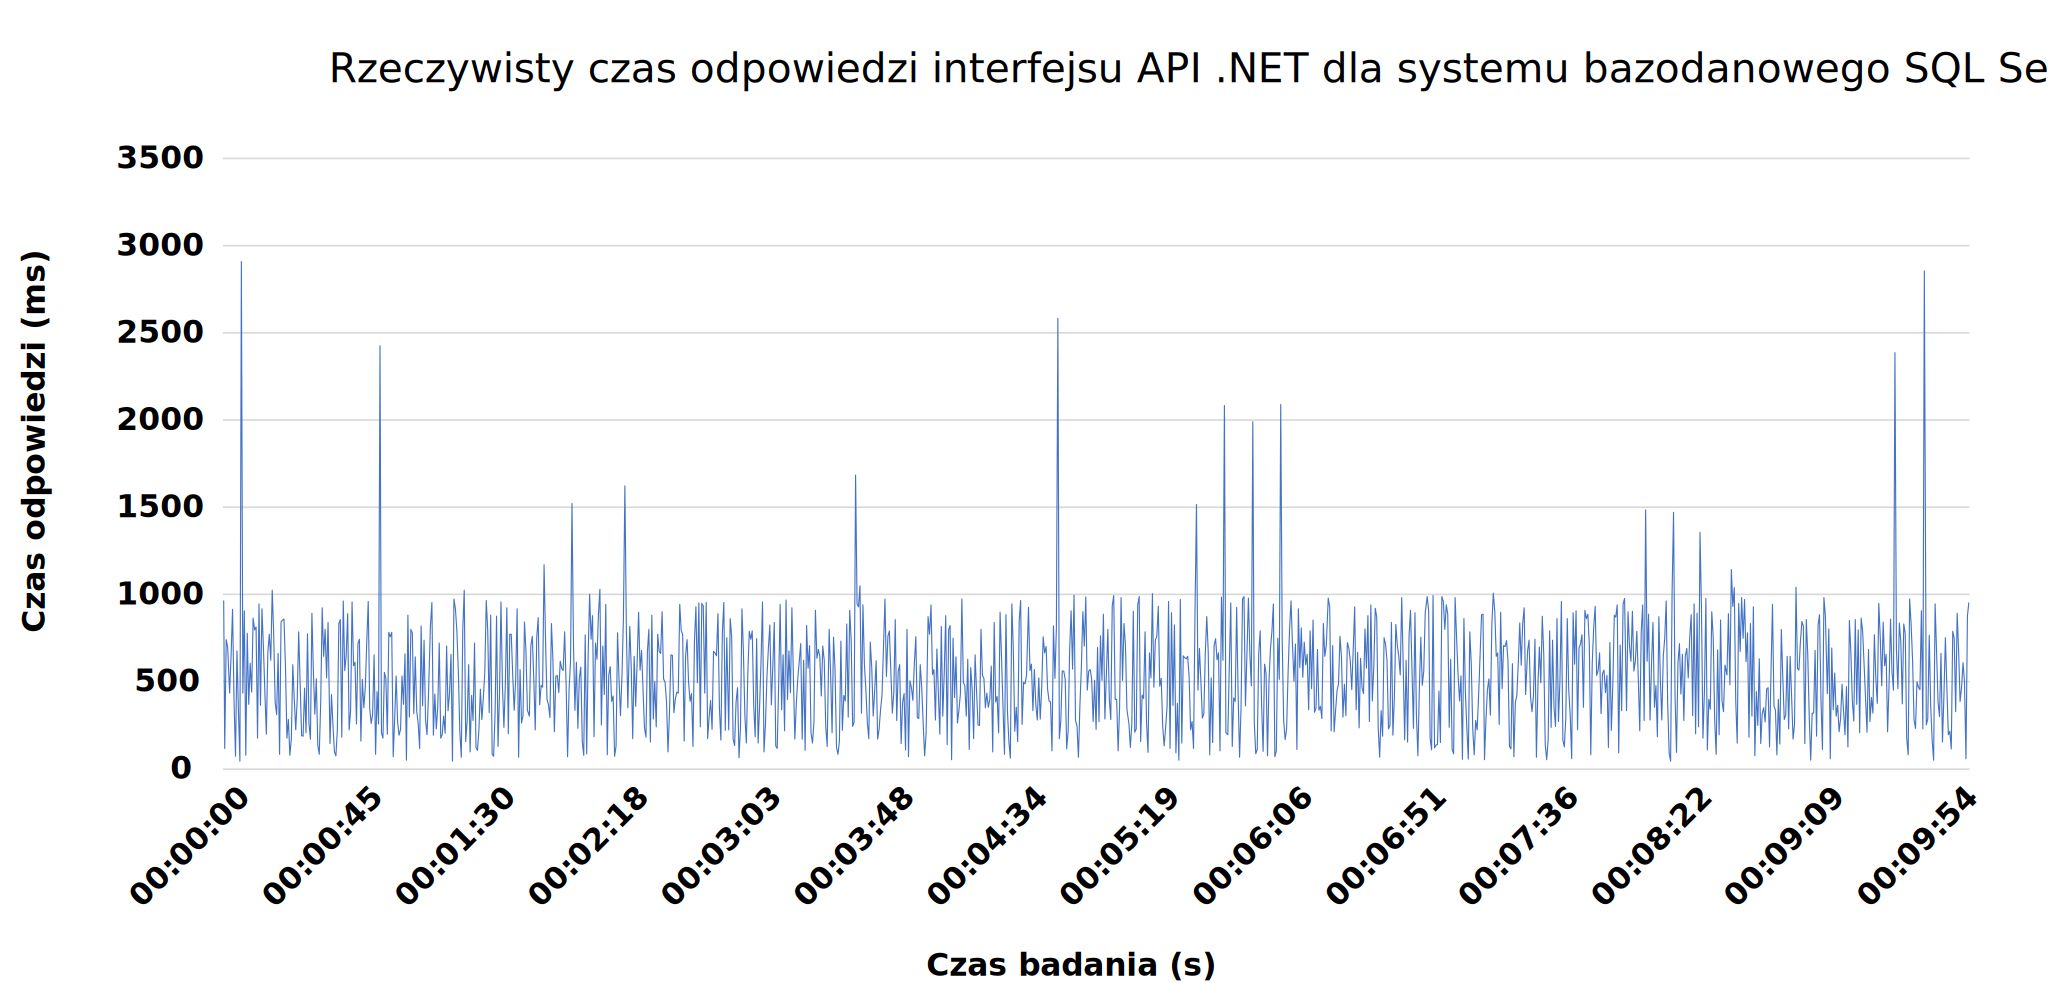
\includegraphics[width=\linewidth]{rys05/testy-funkcjonalne-dotnet.pdf}
    \caption{Czas odpowiedzi na żądanie dla konfiguracji .NET/SQL Server w kontekście testu funkcjonalnego}
    \label{fig:wykres-testy-funkcjonalne-dotnet}
\end{figure}

Na podstawie uzyskanych danych, zdefiniowano progi tolerancji oraz frustracji, wykorzystywane jako punkty odniesienia przy kalkulacji wartości wskaźnika APDEX. Wartości te, ustalono poprzez rosnące posortowanie zbioru czasów odpowiedzi API, a następnie symetryczny podział dwupunktowy. Operacja wykonana została dla każdego z porównywanych systemów bazodanowych w obrębie obu technologii implementacyjnych dotyczących interfejsów API.

Uzyskane przedziały satysfakcji, tolerancji oraz frustracji względem każdego systemu bazodanowego oraz technologii tworzenia API zostały zobrazowane na wykresach \ref{fig:apdex-dotnet} oraz \ref{fig:apdex-nodejs}.

\begin{figure}[ht]
    \centering
     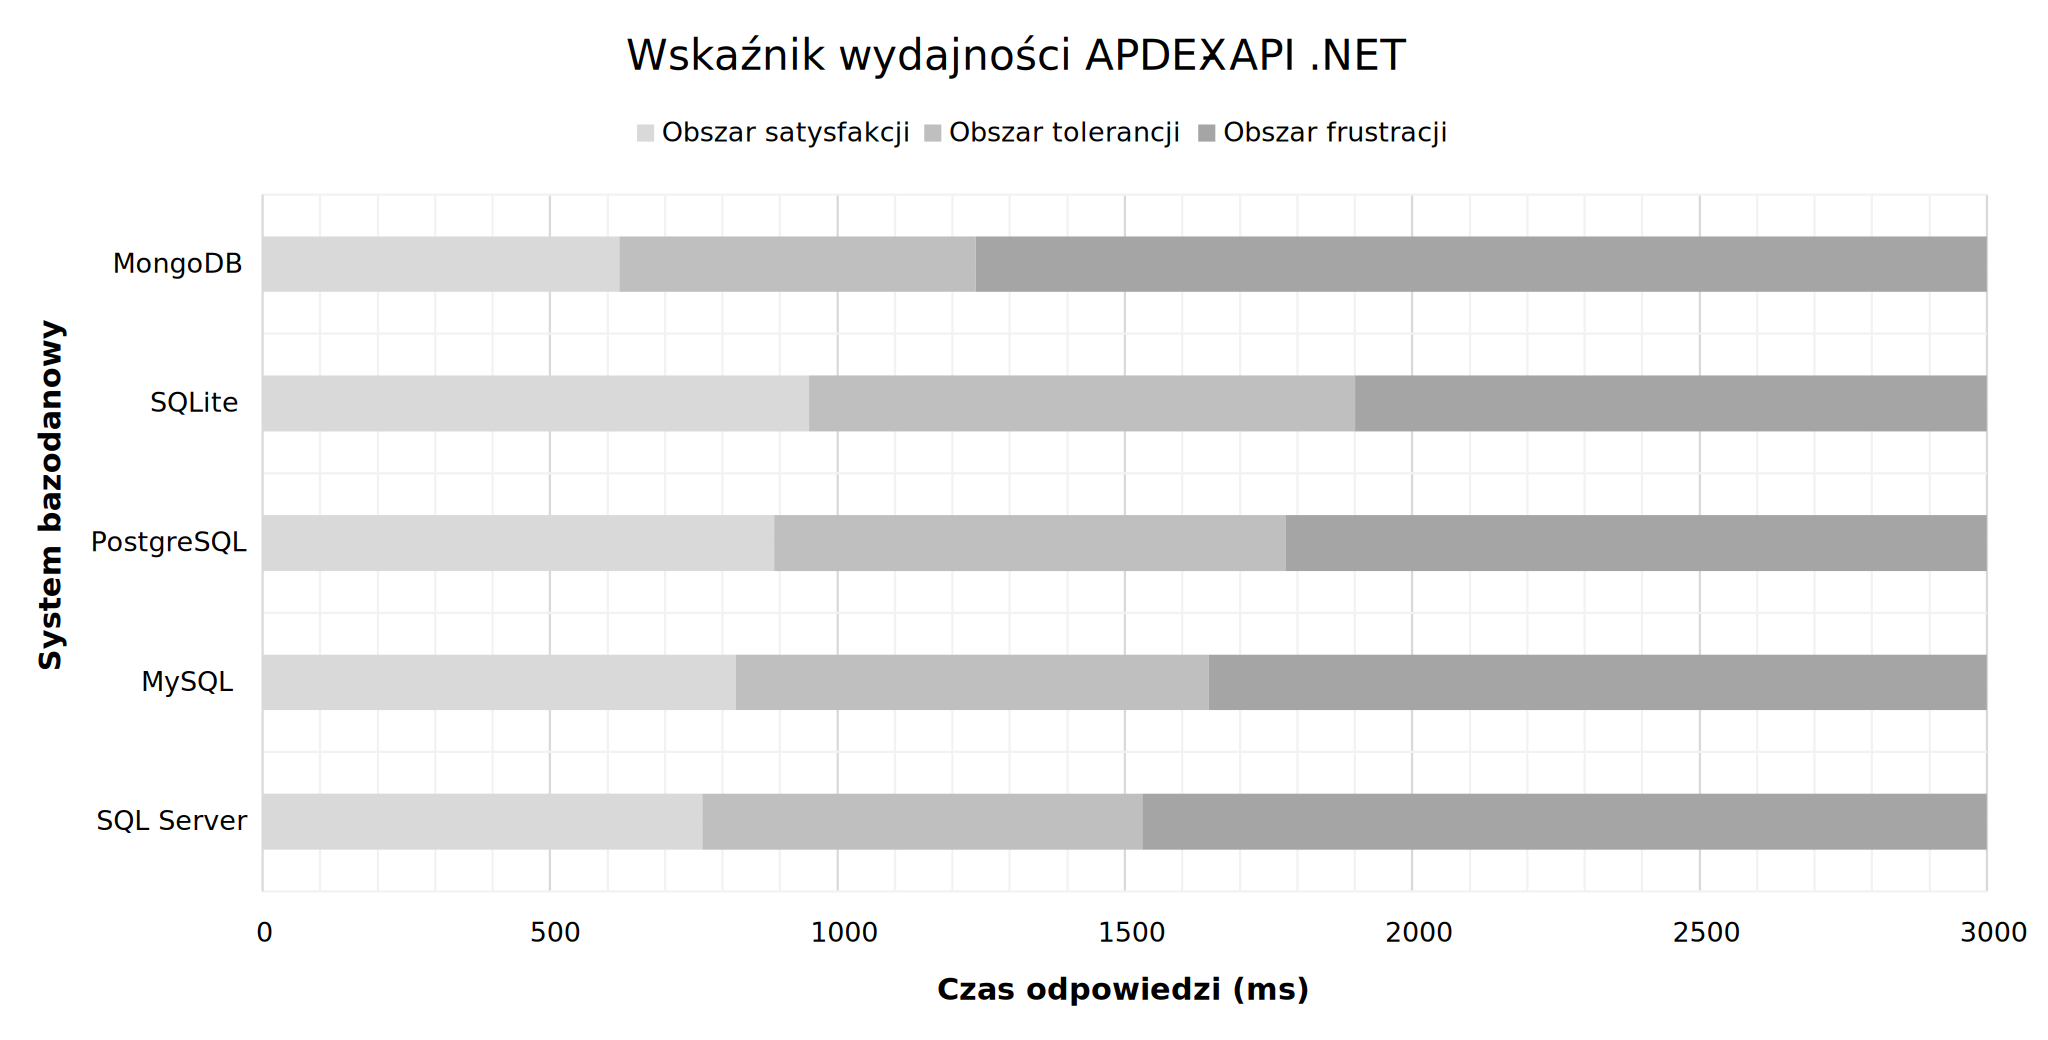
\includegraphics[width=\linewidth]{rys05/apdex-dotnet.pdf}
    \caption{Obszary satysfakcji, tolerancji oraz frustracji wskaźnika APDEX względem poszczególnych systemów bazodanowych dla API zaimplementowanego w C\#}
    \label{fig:apdex-dotnet}
\end{figure}

\begin{figure}[ht]
    \centering
     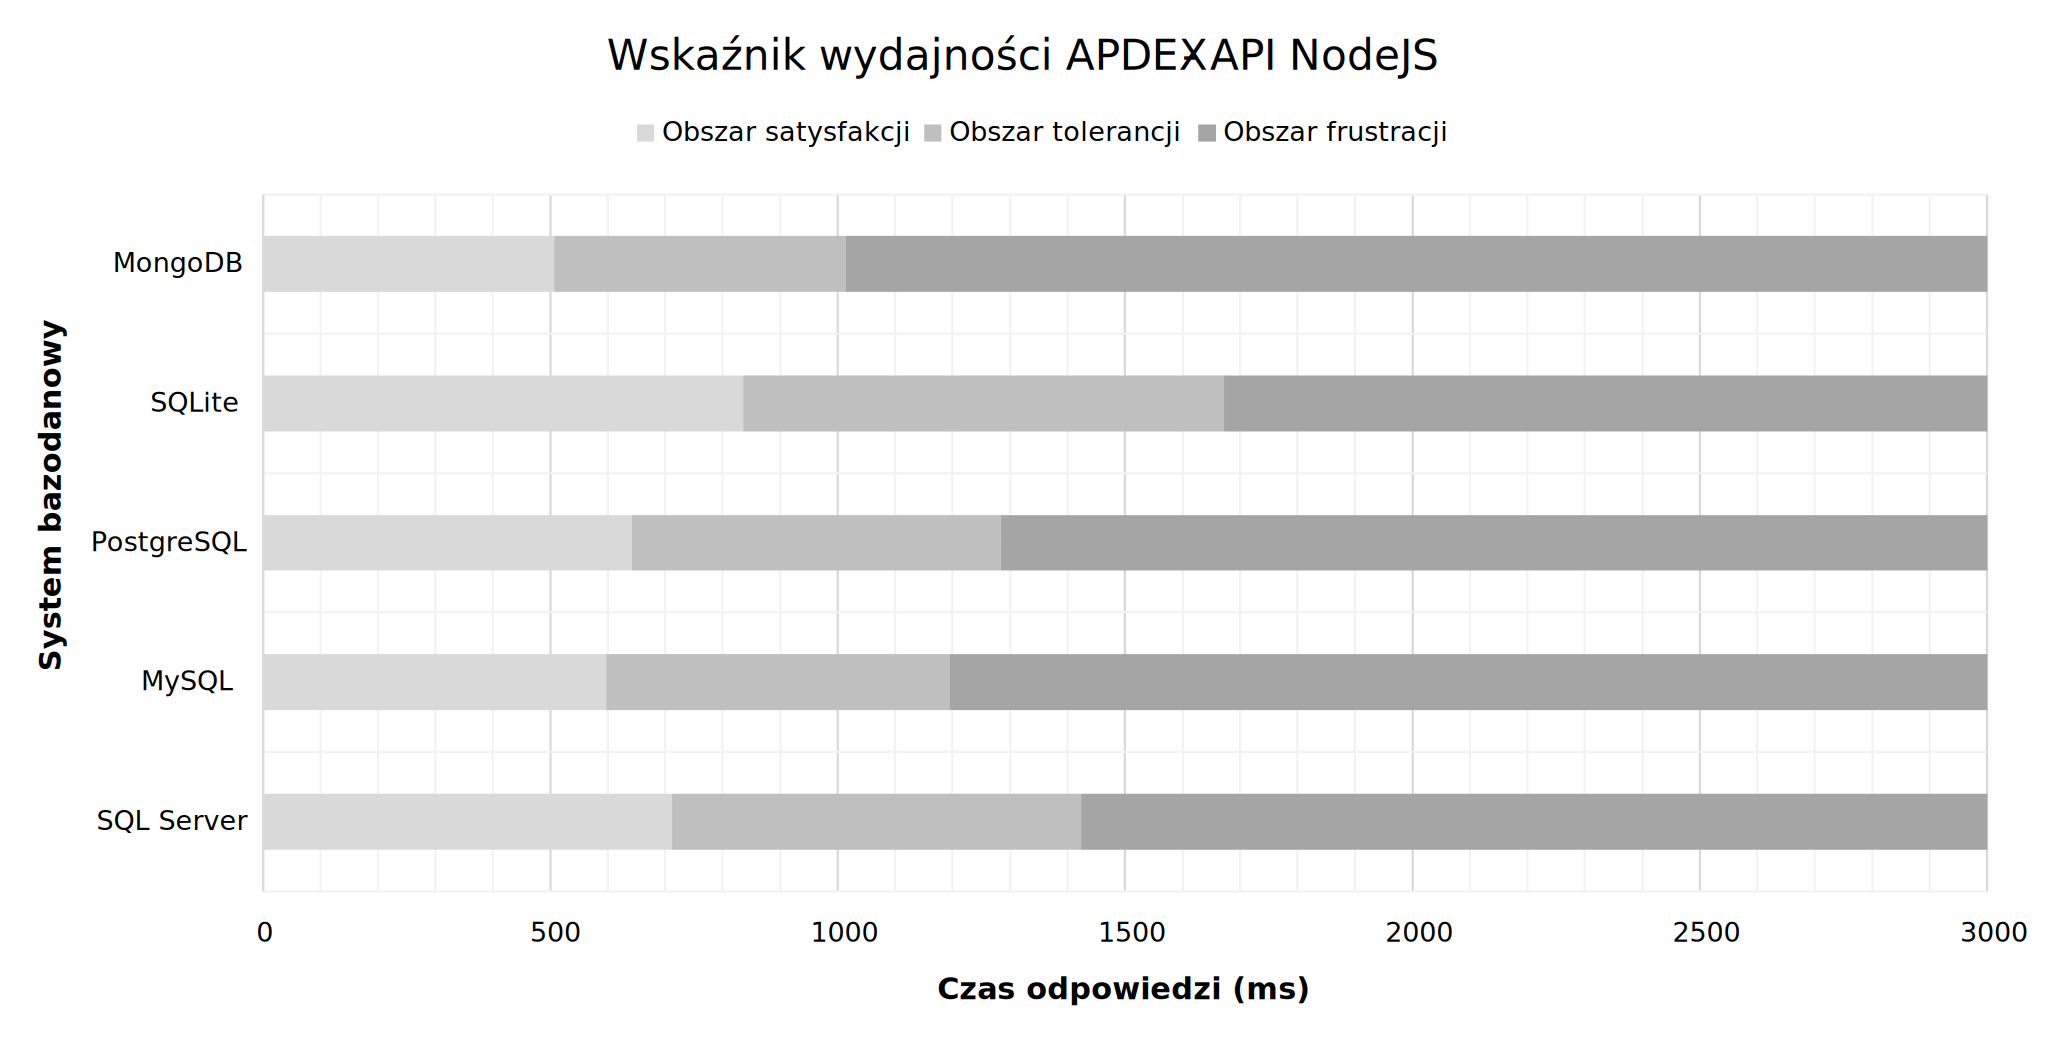
\includegraphics[width=\linewidth]{rys05/apdex-nodejs.pdf}
    \caption{Obszary satysfakcji, tolerancji oraz frustracji wskaźnika APDEX względem poszczególnych systemów bazodanowych dla API zaimplementowanego w JavaScript}
    \label{fig:apdex-nodejs}
\end{figure}

\section{Wpływ zastosowanej technologii programistycznej na wydajność realizacji operacji współbieżnych}
\section{Wpływ zastosowanej technologii programistycznej na efektywność obsługi operacji asynchronicznych}
\section{Wpływ implementacji wzorca projektowego podziału odpowiedzialności na wydajność obsługi żądania klienta}
\section{Porównanie efektywności obsługi żądań klienckich w stałym czasie z uwzględnieniem odmienneych implementacji mechanizmów pamięci podręcznej}
\section{Zmienność wydajności interfejsu API wdrożonego na generycznej oraz dedykowanej platformie chmurowej}
\chapter{Podsumowanie}
\section{Uzyskane efekty pracy}
Celem niniejszej pracy była ewaluacja wydajności interfejsów programowania aplikacji implementowanych w dwóch różnych technologiach, w odniesieniu do licznych aspektów dotyczących sposobów ich wykorzystania. Zdecydowano się nie tylko na analizę efektywności podstawowych rodzajów operacji protokołu hipertekstowego, wchodzących w skład tak popularnych dzisiaj usług sieciowych, ale także wykorzystania mechanizmów programowania współbieżnego, technik obsługi żądań asynchronicznych, implementacji zaawansowanego wzorca projektowego, zastosowania rozwiniętych technik optymalizacji pozyskiwania danych, a także wdrożenia rozwiązań w kontekście środowisk chmurowych.

Zwrócenie uwagi na tak wiele aspektów dotyczących interfejsów programowania aplikacji miało na celu uświadomienie czytelnika, że tego typu systemy internetowe, wykorzystywane są powszechnie nie tylko do realizacji najpopularniejszych czterech, podstawowych operacji na danych. Wachlarz możliwości związanych z tworzeniem internetowych API jest znacząco szerszy, a fakt ten uwydatnia się wraz z rosnącym poziomem skomplikowania usług sieciowych, a także zadań, które są przed nimi stawiane.

Zastosowanie mnogości kontekstów, w których odnaleźć musiały się przygotowane rozwiązania miało również odmienny cel. Misją autora było dowiedzenie się czy którykolwiek z systemów opartych o dwie porównywane technologie wdrożeniowo-uruchomieniowe, wykazuje wysoką wydajność względem swojego konkurenta w którymkolwiek z obszarów prowadzonych badań. Jeżeli tak, to które z tych obszarów są faworyzowane przez konkretne technologie.

Wyniki przeprowadzonych badań umożliwiły rozwianie powyższych wątpliwości, a także uzyskanie dodatkowej wiedzy, która nawet dla osób posiadających doświadczenie w zakresie kompozycji oraz tworzenia interfejsów API nie musi wydawać się oczywista. Zrealizowane eksperymenty uwidoczniły niektóre zależności, zadając innym z kolei kłam. Przykładem potwierdzenia spodziewanej hipotezy, może być wykazana wyższość wydajności rozwiązań implementowanych na platformach dedykowanych względem platform generycznych. Kolejną egzemplifikacją, w ramach której, jeszcze przed przeprowadzeniem badania, sformułować można było silną hipotezę, była obserwacja wpływu zastosowania usprawnień wydajnościowych, separacji środowisk bazodanowych, a także wdrożenia wzorca podziału odpowiedzialności. Rezultaty badania systemów bazodanowych z kolei, mogą być doskonałym argumentem, na obalenie hipotezy wyższej efektywności komunikacji silników baz danych oraz interfejsów tworzonych na bazie technologii jednego producenta.

Odnosząc się do dodatkowej wiedzy, której chęć pozyskiwania wzmożona została poprzez ambicję wyjaśnienia pojawiających się w badaniach anomalii, wspomnieć należy o sposobie obsługi wielowątkowej w odniesieniu do współbieżnie generowanych, długotrwających żądań. Obsługa ta niemalże nie występuje w kontekście interfejsu języka JavaScript, natomiast jest wydatnie rozbudowana w przypadku usługi implementowanej w C\# i uruchamianej na platformie .NET. Ponadto ciekawym jest również fakt, jak bardzo prostota, tycząca się mechanizmów wywoływania operacji asynchronicznych, może nieść korzyść dotyczącą wydajności ich realizacji.

W niektórych przypadkach jednak konwencjonalność rozwiązania nie idzie w parze z jego wydajnością. Potwierdzeniem tego właśnie stwierdzenia są przeprowadzone badania dotyczące podstawowego oraz autorskiego podejścia do realizacji mechanizmów pamięci podręcznej. W ramach pracy tej, zaimplementowano, a także zbadano zachowanie systemu cache uwzględniającego częstotliwość wywoływania punktu końcowego, a także liczbę unieważnień identyfikującego go wpisu. Zgromadzone rezultaty należy postrzegać jako obiecujące, jednakże wymagana jest zdecydowanie bardzej obszerna analiza uwzględniająca zmienność liczby momentów unieważnień, czy też wpływ dysproporcji parametrów w różnych chwilach obsługi żądań.

Wspomnieć należy również o przeprowadzonych w ramach niniejszego badania parowych testach statystycznych, które pozwoliły na wykazanie statystycznie istotnej przewagi określonych konfiguracji rozwiązań względem pozostałych z nich. 

Bardzo ważnym jest również uwypuklenie pewnej tezy. Przeprowadzony zestaw badań nie wskazał, jednakże przede wszystkim nie miał wskazać, technologii niezaprzeczalnie lepszej. Technologia taka nie istnieje, a wynika to w głównej mierze z ilości obszarów, w kontekście których może ona zostać wykorzystana oraz badana. Dlatego też, dokument ten, może okazać się pomocny dla tych osób, którzy zainteresowani są oceną poziomu wydajności interfejsu dla konkretnej technologii oraz konkretnego sposobu jej wykorzystania.
\section{Perspektywy rozwoju badań}
Każdy z przytoczonych obszarów wykorzystania interfejsów programowania aplikacji, reprezentowany w niniejszej pracy poprzez odmienne badanie, może zostać z łatwością rozbudowany poprzez ewaluację dodatkowych metryk wydajnościowych, czy też zmianę konfiguracji środowiska badawczego. Zdecydowano się na wskazanie perspektyw rozwoju badań w odniesieniu do tych domen funkcjonalności API, które zostały poruszone w tym dokumencie.

Odwołując się do badania wpływu wykorzystania systemów bazodanowych w kontekście porównywanych technologii, jako perspektywę rozwoju wskazać należy przeprowadzenie ewaluacji wydajności dla przedziałów liczby wątków-generatorów o zmiennej długości. Ponadto, wzięte pod uwagę mogą być również te spośród systemów bazodanowych, w ramach których nie dostarczane jest wsparcie dla mapperów obiektowo-relacyjnych Entity Framework Core oraz Prisma.

W ramach badania realizacji operacji współbieżnych, wprowadzić można dodatkowe rodzaje algorytmów metaheurystycznych dla różnych problemów o wysokiej złożoności obliczeniowej. Interesującą perspektywą rozwoju tego badania, jest również implementacja odmiennych heurystyk dla symetrycznego problemu komiwojażera, a także porównanie ich wykonania dla interfejsów wspierających przetwarzanie wielowątkowe.

Badanie wydajności operacji asynchronicznych może zostać poszerzone o uwzględnienie różnych implementacji klientów protokołu hipertekstowego, a także konfiguracji poszczególnych ich parametrów.

Najwięcej perspektyw rozwoju badań, wyróżnić należy w kontekście ewaluacji porównywanych mechanizmów pamięci podręcznej. Zbadane mogą zostać między innymi odmienne metryki wpływające na zmianę czasu odpowiedzi na żądanie. Jako przykładową metrykę wskazać można narzut wydajnościowy wprowadzany przez metodę kalkulacji czasu życia wpisu w magazynie pamięci podręcznej. Ponadto, struktura wykonanego badania, mogłaby zostać dostosowana względem zmiennego czasu trwania testu, zmiennego natężenia ruchu sieciowego, czy też deterministycznego charakteru wywoływania żądań unieważniających. Co więcej, zaproponowana przez autora metoda może zostać zmodyfikowana poprzez uzależnienie czasu przechowywania wpisu od dodatkowych parametrów, bądź też zmianę ich istotności względem wyliczania czasu życia elementu pamięci cache.

W kontekście wprowadzenia wzorca podziału odpowiedzialności, a także separacji modeli bazodanowych, badanie może zostać poszerzone o zastosowanie odmiennych mechanizmów replikacji, niż wykorzystana w tej pracy technika transakcyjna. W takim przypadku, należy zbadać w jakim czasie, od momentu dodania rekordu bazodanowego, będzie on dostępny w ramach źródła danych przeznaczonego do odczytu. Co więcej, należy pamiętać, że celem zdefiniowania specyficznej struktury obsługi żądania, była możliwość optymalizacji modeli danych. Dlatego też, interesującą perspektywą rozwoju tego badania, mogłoby być wskazanie, które z zaimplementowanych technik optymalizacji mają kluczowe znaczenie pod kątem wydajności, a które wpływają na nią jedynie nieznacznie.

Ostatnie ze zidentyfikowanych perspektyw rozwoju tyczą się obserwacji efektywności działania w odniesieniu do produkcyjnych środowisk chmurowych. Biorąc pod uwagę ten właśnie aspekt, możliwym jest dokonanie porównania dla większej liczby platform wdrożeniowych, czy też zbadanie, w jaki sposób usługi generyczne typu infrastructure-as-a-service mogą zostać zoptymalizowane, aby implementowane wewnątrz nich systemy internetowe, osiągały wydajność przybliżoną, lub wyższą względem rozwiązań dedykowanych. 


%\bibliographystyle{plalpha}
\bibliographystyle{plabbrv}

%UWAGA: bibliotekę referencji należy przygotować samemu. Dobrym do tego narzędziem jest JabRef.
%       Nazwę przygotowanej biblioteki wpisuje się poniżej bez rozszerzenia 
%       (w tym przypadku jest to "dokumentacja.bib")
\setlength{\bibitemsep}{2pt} % - by zacieśnić wykaz literatury
\bibliography{dokumentacja}

\end{document}
